% Options for packages loaded elsewhere
% Options for packages loaded elsewhere
\PassOptionsToPackage{unicode}{hyperref}
\PassOptionsToPackage{hyphens}{url}
\PassOptionsToPackage{dvipsnames,svgnames,x11names}{xcolor}
%
\documentclass[
  letterpaper,
  DIV=11,
  numbers=noendperiod]{scrreprt}
\usepackage{xcolor}
\usepackage{amsmath,amssymb}
\setcounter{secnumdepth}{5}
\usepackage{iftex}
\ifPDFTeX
  \usepackage[T1]{fontenc}
  \usepackage[utf8]{inputenc}
  \usepackage{textcomp} % provide euro and other symbols
\else % if luatex or xetex
  \usepackage{unicode-math} % this also loads fontspec
  \defaultfontfeatures{Scale=MatchLowercase}
  \defaultfontfeatures[\rmfamily]{Ligatures=TeX,Scale=1}
\fi
\usepackage{lmodern}
\ifPDFTeX\else
  % xetex/luatex font selection
\fi
% Use upquote if available, for straight quotes in verbatim environments
\IfFileExists{upquote.sty}{\usepackage{upquote}}{}
\IfFileExists{microtype.sty}{% use microtype if available
  \usepackage[]{microtype}
  \UseMicrotypeSet[protrusion]{basicmath} % disable protrusion for tt fonts
}{}
\makeatletter
\@ifundefined{KOMAClassName}{% if non-KOMA class
  \IfFileExists{parskip.sty}{%
    \usepackage{parskip}
  }{% else
    \setlength{\parindent}{0pt}
    \setlength{\parskip}{6pt plus 2pt minus 1pt}}
}{% if KOMA class
  \KOMAoptions{parskip=half}}
\makeatother
% Make \paragraph and \subparagraph free-standing
\makeatletter
\ifx\paragraph\undefined\else
  \let\oldparagraph\paragraph
  \renewcommand{\paragraph}{
    \@ifstar
      \xxxParagraphStar
      \xxxParagraphNoStar
  }
  \newcommand{\xxxParagraphStar}[1]{\oldparagraph*{#1}\mbox{}}
  \newcommand{\xxxParagraphNoStar}[1]{\oldparagraph{#1}\mbox{}}
\fi
\ifx\subparagraph\undefined\else
  \let\oldsubparagraph\subparagraph
  \renewcommand{\subparagraph}{
    \@ifstar
      \xxxSubParagraphStar
      \xxxSubParagraphNoStar
  }
  \newcommand{\xxxSubParagraphStar}[1]{\oldsubparagraph*{#1}\mbox{}}
  \newcommand{\xxxSubParagraphNoStar}[1]{\oldsubparagraph{#1}\mbox{}}
\fi
\makeatother


\usepackage{longtable,booktabs,array}
\newcounter{none} % for unnumbered tables
\usepackage{calc} % for calculating minipage widths
% Correct order of tables after \paragraph or \subparagraph
\usepackage{etoolbox}
\makeatletter
\patchcmd\longtable{\par}{\if@noskipsec\mbox{}\fi\par}{}{}
\makeatother
% Allow footnotes in longtable head/foot
\IfFileExists{footnotehyper.sty}{\usepackage{footnotehyper}}{\usepackage{footnote}}
\makesavenoteenv{longtable}
\usepackage{graphicx}
\makeatletter
\newsavebox\pandoc@box
\newcommand*\pandocbounded[1]{% scales image to fit in text height/width
  \sbox\pandoc@box{#1}%
  \Gscale@div\@tempa{\textheight}{\dimexpr\ht\pandoc@box+\dp\pandoc@box\relax}%
  \Gscale@div\@tempb{\linewidth}{\wd\pandoc@box}%
  \ifdim\@tempb\p@<\@tempa\p@\let\@tempa\@tempb\fi% select the smaller of both
  \ifdim\@tempa\p@<\p@\scalebox{\@tempa}{\usebox\pandoc@box}%
  \else\usebox{\pandoc@box}%
  \fi%
}
% Set default figure placement to htbp
\def\fps@figure{htbp}
\makeatother
\usepackage{svg}

\ifLuaTeX
  \usepackage{luacolor}
  \usepackage[soul]{lua-ul}
\else
  \usepackage{soul}
\fi

% definitions for citeproc citations
\NewDocumentCommand\citeproctext{}{}
\NewDocumentCommand\citeproc{mm}{%
  \begingroup\def\citeproctext{#2}\cite{#1}\endgroup}
\makeatletter
 % allow citations to break across lines
 \let\@cite@ofmt\@firstofone
 % avoid brackets around text for \cite:
 \def\@biblabel#1{}
 \def\@cite#1#2{{#1\if@tempswa , #2\fi}}
\makeatother
\newlength{\cslhangindent}
\setlength{\cslhangindent}{1.5em}
\newlength{\csllabelwidth}
\setlength{\csllabelwidth}{3em}
\newenvironment{CSLReferences}[2] % #1 hanging-indent, #2 entry-spacing
 {\begin{list}{}{%
  \setlength{\itemindent}{0pt}
  \setlength{\leftmargin}{0pt}
  \setlength{\parsep}{0pt}
  % turn on hanging indent if param 1 is 1
  \ifodd #1
   \setlength{\leftmargin}{\cslhangindent}
   \setlength{\itemindent}{-1\cslhangindent}
  \fi
  % set entry spacing
  \setlength{\itemsep}{#2\baselineskip}}}
 {\end{list}}
\usepackage{calc}
\newcommand{\CSLBlock}[1]{\hfill\break\parbox[t]{\linewidth}{\strut\ignorespaces#1\strut}}
\newcommand{\CSLLeftMargin}[1]{\parbox[t]{\csllabelwidth}{\strut#1\strut}}
\newcommand{\CSLRightInline}[1]{\parbox[t]{\linewidth - \csllabelwidth}{\strut#1\strut}}
\newcommand{\CSLIndent}[1]{\hspace{\cslhangindent}#1}



\setlength{\emergencystretch}{3em} % prevent overfull lines

\providecommand{\tightlist}{%
  \setlength{\itemsep}{0pt}\setlength{\parskip}{0pt}}



 


\KOMAoption{captions}{tableheading}
\makeatletter
\@ifpackageloaded{tcolorbox}{}{\usepackage[skins,breakable]{tcolorbox}}
\@ifpackageloaded{fontawesome5}{}{\usepackage{fontawesome5}}
\definecolor{quarto-callout-color}{HTML}{909090}
\definecolor{quarto-callout-note-color}{HTML}{0758E5}
\definecolor{quarto-callout-important-color}{HTML}{CC1914}
\definecolor{quarto-callout-warning-color}{HTML}{EB9113}
\definecolor{quarto-callout-tip-color}{HTML}{00A047}
\definecolor{quarto-callout-caution-color}{HTML}{FC5300}
\definecolor{quarto-callout-color-frame}{HTML}{acacac}
\definecolor{quarto-callout-note-color-frame}{HTML}{4582ec}
\definecolor{quarto-callout-important-color-frame}{HTML}{d9534f}
\definecolor{quarto-callout-warning-color-frame}{HTML}{f0ad4e}
\definecolor{quarto-callout-tip-color-frame}{HTML}{02b875}
\definecolor{quarto-callout-caution-color-frame}{HTML}{fd7e14}
\makeatother
\makeatletter
\@ifpackageloaded{bookmark}{}{\usepackage{bookmark}}
\makeatother
\makeatletter
\@ifpackageloaded{caption}{}{\usepackage{caption}}
\AtBeginDocument{%
\ifdefined\contentsname
  \renewcommand*\contentsname{Table of contents}
\else
  \newcommand\contentsname{Table of contents}
\fi
\ifdefined\listfigurename
  \renewcommand*\listfigurename{List of Figures}
\else
  \newcommand\listfigurename{List of Figures}
\fi
\ifdefined\listtablename
  \renewcommand*\listtablename{List of Tables}
\else
  \newcommand\listtablename{List of Tables}
\fi
\ifdefined\figurename
  \renewcommand*\figurename{Figure}
\else
  \newcommand\figurename{Figure}
\fi
\ifdefined\tablename
  \renewcommand*\tablename{Table}
\else
  \newcommand\tablename{Table}
\fi
}
\@ifpackageloaded{float}{}{\usepackage{float}}
\floatstyle{ruled}
\@ifundefined{c@chapter}{\newfloat{codelisting}{h}{lop}}{\newfloat{codelisting}{h}{lop}[chapter]}
\floatname{codelisting}{Listing}
\newcommand*\listoflistings{\listof{codelisting}{List of Listings}}
\makeatother
\makeatletter
\makeatother
\makeatletter
\@ifpackageloaded{caption}{}{\usepackage{caption}}
\@ifpackageloaded{subcaption}{}{\usepackage{subcaption}}
\makeatother
\usepackage{bookmark}
\IfFileExists{xurl.sty}{\usepackage{xurl}}{} % add URL line breaks if available
\urlstyle{same}
% fallback for those not using the hyperref driver hyperxmp:
\makeatletter
\@ifundefined{xmpquote}{\newcommand{\xmpquote}[1]{#1}}{}
\makeatother
\hypersetup{
  pdftitle={Information in Society},
  pdfauthor={Philippe Mongeon},
  colorlinks=true,
  linkcolor={blue},
  filecolor={Maroon},
  citecolor={Blue},
  urlcolor={Blue},
  pdfcreator={LaTeX via pandoc}}


\title{Information in Society}
\author{Philippe Mongeon}
\date{2022-08-26}
\begin{document}
\maketitle

\renewcommand*\contentsname{Table of contents}
{
\setcounter{tocdepth}{2}
\tableofcontents
}

\bookmarksetup{startatroot}

\chapter{Course Overview}\label{course-overview}

\bookmarksetup{startatroot}

\chapter{Learning Outcomes}\label{learning-outcomes}

Upon completion of this course, students should be able to:

\begin{itemize}
\tightlist
\item
  Explain the general significance of information in contemporary
  society.
\item
  Provide an informed and critical perspective on information phenomena
  and processes.
\item
  Understand the nature and social roles of the information professions.
\item
  Identify contemporary issues and their relationship with information
  and the information field.
\end{itemize}

\bookmarksetup{startatroot}

\chapter{Course Schedule}\label{course-schedule}

{\def\LTcaptype{none} % do not increment counter
\begin{longtable}[]{@{}
  >{\centering\arraybackslash}p{(\linewidth - 4\tabcolsep) * \real{0.3537}}
  >{\raggedright\arraybackslash}p{(\linewidth - 4\tabcolsep) * \real{0.3171}}
  >{\raggedright\arraybackslash}p{(\linewidth - 4\tabcolsep) * \real{0.3252}}@{}}
\toprule\noalign{}
\begin{minipage}[b]{\linewidth}\centering
Date
\end{minipage} & \begin{minipage}[b]{\linewidth}\raggedright
Theme/reading to complete before class
\end{minipage} & \begin{minipage}[b]{\linewidth}\raggedright
Class activities
\end{minipage} \\
\midrule\noalign{}
\endhead
\bottomrule\noalign{}
\endlastfoot
Sep 14 & \href{content/ch1.qmd}{Chapter 1. The Information Field} &
\begin{minipage}[t]{\linewidth}\raggedright
Introduction\\
Course overview\strut
\end{minipage} \\
Sep 21 & \href{content/ch2.qmd}{Chapter 2. What is Information?} &
\begin{minipage}[t]{\linewidth}\raggedright
Short lecture\\
group exercise\strut
\end{minipage} \\
Sep 28 & \href{content/ch3.qmd}{Chapter 3. Information Issues} & Guest
lecture by Dr.~Jennifer Grek-Martin \\
Oct 5 & \href{content/ch10.qmd}{Chapter 10. Information and Democracy} &
Guest lecture by Dr.~Jason Hannan \\
\begin{minipage}[t]{\linewidth}\centering
Oct 19\\
\href{https://teams.microsoft.com/meet/2552696644987515?p=AvGabNhUaWWAirpCh6}{Teams
link}\strut
\end{minipage} & \begin{minipage}[t]{\linewidth}\raggedright
\href{content/ch5.qmd}{Chapter 5. Work in the Information Society}\\
\href{content/ch6.qmd}{Chapter 6. Information in Organizations}\strut
\end{minipage} & Guest lecture by Kellie Dalton

\href{https://pmongeon.github.io/information-in-society/slides/week5.html}{slides} \\
\begin{minipage}[t]{\linewidth}\centering
Oct 26\\
\href{https://teams.microsoft.com/meet/225771196342159?p=mYWVwqquIataLxPT7Z}{Teams
link}\strut
\end{minipage} & \href{content/ch7.qmd}{Chapter 7. The Information
Economy} & Guest lecture by Dan Philips \\
\begin{minipage}[t]{\linewidth}\centering
Nov 2\\
\href{https://teams.microsoft.com/meet/2493505198739147?p=8nOzjwqIeaxzQRxuIC}{Teams
link}\strut
\end{minipage} & \begin{minipage}[t]{\linewidth}\raggedright
\href{content/ch4.qmd}{Chapter 4. Humans in an Information Society}\\
\href{content/ch8.qmd}{Chapter 8. The Attention Economy}\strut
\end{minipage} & Short lecture + group discussions \\
\begin{minipage}[t]{\linewidth}\centering
Nov 16\\
\href{https://teams.microsoft.com/meet/210546465672495?p=IpMSVpp2llEfK80C1l}{Teams
link}\strut
\end{minipage} & \href{content/ch11.qmd}{Chapter 11. Information
Justice} & Guest lecture by Alison Brown \\
\begin{minipage}[t]{\linewidth}\centering
Nov 23\\
\href{https://teams.microsoft.com/meet/210546465672495?p=IpMSVpp2llEfK80C1l}{Teams
link}\strut
\end{minipage} & TBD & Guest lecture by Maddie Hare and Janet Music \\
\begin{minipage}[t]{\linewidth}\centering
Nov 30\\
\href{https://teams.microsoft.com/meet/2857907700956468?p=NGq7QGL8UuYBB7hidg}{Teams
link}\strut
\end{minipage} & \href{content/ch9.qmd}{Chapter 9. Misinformation,
Disinformation, and Fake News} &
\begin{minipage}[t]{\linewidth}\raggedright
Short lecture\\
group exercise\strut
\end{minipage} \\
\begin{minipage}[t]{\linewidth}\centering
Dec 7\\
\href{https://teams.microsoft.com/meet/265440625779680?p=1Uk0fwl3Pj6VKOnDuB}{Teams
link}\strut
\end{minipage} & TBD & Guest lecture by Coel Conrad \\
\begin{minipage}[t]{\linewidth}\centering
Dec 8\\
\href{https://teams.microsoft.com/meet/2144650994710788?p=gFnPwpCcDWSU92Tj0l}{Teams
link}\strut
\end{minipage} & N/A & Fun. \\
\end{longtable}
}

\bookmarksetup{startatroot}

\chapter{Assignments}\label{assignments}

\textbf{IMPORTANT NOTE:} The assignments will be updated in the next few
days, the current ones reflect essentially what the assignments will be
for this course, but be aware that they will slightly change.

{\def\LTcaptype{none} % do not increment counter
\begin{longtable}[]{@{}
  >{\raggedright\arraybackslash}p{(\linewidth - 4\tabcolsep) * \real{0.3333}}
  >{\raggedright\arraybackslash}p{(\linewidth - 4\tabcolsep) * \real{0.3333}}
  >{\raggedright\arraybackslash}p{(\linewidth - 4\tabcolsep) * \real{0.3333}}@{}}
\toprule\noalign{}
\begin{minipage}[b]{\linewidth}\raggedright
Assignment
\end{minipage} & \begin{minipage}[b]{\linewidth}\raggedright
Due date
\end{minipage} & \begin{minipage}[b]{\linewidth}\raggedright
Weight
\end{minipage} \\
\midrule\noalign{}
\endhead
\bottomrule\noalign{}
\endlastfoot
\href{assignments/0-participation.qmd}{Participation self-assessment -
Part 1} & Friday, September 25, 2026 & 7.5\% \\
\href{assignments/1-information-setting.qmd}{Analysis of an information
setting} & Friday, October 16, 2026 & 30\% \\
\href{assignments/0-participation.qmd}{Participation self-assessment -
Part 2} & Friday, October 30, 2026 & 5\% \\
\href{assignments/2-essay-plan.qmd}{Essay plan} & Friday, October 30,
2026 & 10\% \\
\href{assignments/3-essay.qmd}{Essay} & Friday, December 11, 2026 &
40\% \\
\href{assignments/0-participation.qmd}{Participation self-assessment -
Part 3} & Friday, December 11, 2026 & 7.5\% \\
\end{longtable}
}

\bookmarksetup{startatroot}

\chapter{Other Important Information and
Resources}\label{other-important-information-and-resources}

\begin{itemize}
\tightlist
\item
  You can access this course website without going through Brightspace
  with the following URL:
  \url{https://pmongeon.github.io/information-in-society/}.
\item
  The official \href{files/INFO5500-Syllabus.pdf}{course syllabus}.
\item
  A
  \href{https://www.zotero.org/groups/2536626/info5500_-_information_in_society/library}{Zotero
  library} with all the references in the course website, organized by
  chapter.
\item
  Use \href{https://www.zotero.org}{Zotero} (or another reference
  manager of your choice) to store your references and cite them in your
  work. (not mandatory, but highly recommended).
\item
  Use \textbf{APA style} for your references in all assignments.
\item
  You can use this \href{files/assignment-template.dotx}{Word template}
  to write your assignments (not mandatory). Whether you use this
  template or not, I strongly recommend using Word styles to format and
  structure your document.
\item
  Have fun.
\end{itemize}

\bookmarksetup{startatroot}

\chapter{Acknowledgements}\label{acknowledgements}

The textbook would not have been possible without the financial support,
through an OER grant, of the
\href{https://www.dal.ca/dept/clt.html}{Dalhousie Center for Learning
and Teaching} and the \href{https://libraries.dal.ca/}{Dalhousie
Libraries}. It also would not have been possible without the help and
support of Dr.~Samantha Taylor, senior instructor and co-lead on the
project, who orchestrated the writing of the case studies included
throughout the book. It also would not have been possible without the
hard work of Janine McGregor, Maddie Hare, Poppy Riddle, and Tessa
Biesterfeld, alumni from Dalhousie's Master of Information program, who
wrote the case studies and helped draft some of the chapters. Special
thanks to Janine McGregor, who played a leading role in the planning and
writing of the textbook.

\bookmarksetup{startatroot}

\chapter{The Information Field}\label{the-information-field}

\section{Learning objectives}\label{learning-objectives}

This introductory chapter aims to provide an overview of the diverse
range of professional pathways to which your ALA-accredited information
management program can lead you. As we will see in this chapter,
information management degrees are about a lot more than librarianship
and can provide you with many opportunities. This chapter will give you
an overview of the roles that information professionals can play in
various sectors and provide some resources to help you think about your
own interests and development pathways.

\section{What is the information
field?}\label{what-is-the-information-field}

The Master of Information, like other similar programs offered in Canada
and the United States, is often associated with libraries and
librarianship (and rightfully so) because of its accreditation by the
American Library Association (ALA). ALA-accredited degrees are generally
a requirement for a range of positions in libraries of all kinds and
other related organizations. Accordingly, most students reading this
chapter will likely be interested in pursuing a career in librarianship.
Many of you, however, are in this program with completely different
careers in mind, and you may be surprised by the emphasis on libraries.
Perhaps some of you have no prior thoughts about the program or the
field as you are taking this course as an elective or simply because you
ended up here randomly. Those of you in the Master of Information
Management program, which is \textbf{not} ALA-accredited, are likely
mid-career professionals working in a wide range of sectors. Whatever
group you find yourself in, now that you are here, you might be
surprised by the breadth of the discipline and the many professional
pathways it can lead you on. Maybe you joined the program to be a
children services librarian and will come out of it as an aspiring data
scientist\ldots who knows?

So, what is the information field? Bates (2015) referred to our
discipline as a meta-discipline that spans the entire spectrum of
traditional research disciplines, from the Arts and Humanities to
Natural Sciences. While it is not comprehensive, this figure from Bates
(2015) was an attempt to illustrate the breadth of the discipline by
situating many of the sub-disciplines across that spectrum.

\begin{figure}[H]

{\centering 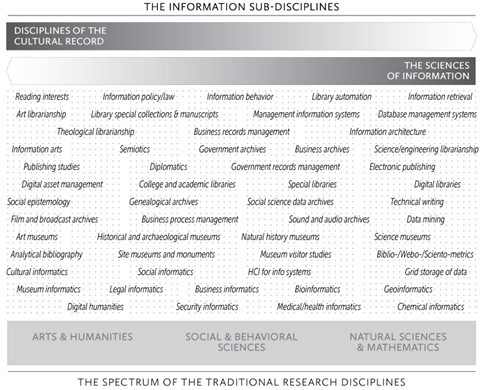
\includegraphics[width=6.80208in,height=\textheight,keepaspectratio]{content/images/ch1-fig1.jpg}

}

\caption{Figure 1.1. The information sub-fields (Bates 2015)}

\end{figure}%

\section{Core competencies}\label{core-competencies}

Regardless of your professional path or the sector in which you find
employment. There are a set of competencies that are core to our field.
These are visible through the core competencies lists that you will find
on the website of most academic units offering ALA-accredited programs.
Here are the MI competencies published on the program's website:

\begin{enumerate}
\def\labelenumi{\arabic{enumi}.}
\item
  \textbf{Adaptation}: Information managers anticipate and adapt to
  trends in information management, support organizational change, and
  promote a learning culture within the organization.
\item
  \textbf{Collaboration}: Information managers work effectively in
  teams, cultivate a collaborative culture within the organization, and
  build relationships with stakeholders.
\item
  \textbf{Commitment to equity, diversity, inclusion, accessibility, and
  decolonization}: Information managers practice and critique the
  principles of equity, diversity, inclusion, accessibility, and
  decolonization for participating in an inclusive and socially just
  society.
\item
  \textbf{Communication:} Information managers communicate effectively,
  listen actively, and are receptive to feedback and suggestions.
\item
  \textbf{Digital and technological literacy}: Information managers
  safely, responsibly, creatively, and effectively use technologies.
  They assess the organization's or users' IT requirements and develop
  and implement IT strategies that support the organization's mission.
\item
  \textbf{Evidence-based practices}: Information managers promote
  evidence-based decision-making and policies. They use adequate methods
  to produce, assess, synthesize, and evaluate knowledge to support the
  organization's activities.
\item
  \textbf{Leadership}: Information managers advocate the strategic
  importance of information for their organization or community, promote
  the professional values of the field, support the development of their
  peers, and mobilize people and resources toward achieving collective
  goals.
\item
  \textbf{Learning}: Information managers are reflexive, life-long
  learners who adopt a creative and innovative approach to their work.
\item
  \textbf{Management}: Information managers effectively manage projects,
  people and resources and ensure that the information assets and
  practices of the organization support its values, mission and
  objectives.
\item
  \textbf{User-centered design}: Information Managers engage users and
  adapt services to their information needs and behaviours.
\end{enumerate}

\section{Roles, values and
principles}\label{roles-values-and-principles}

The information professions fulfill a wide range of societal and
organizational roles. All organizations produce and need information to
support their operation. They \textbf{support the day-to-day activities
of organizations} by collecting and organizing data, documents, and
archives and by managing information systems, among other tasks.
Information professionals also have an \textbf{educational role}, which
they often fulfill by providing data, information literacy, and
information technology training to patrons in public libraries,
students, and colleagues in any work environment and by gathering and
organizing teaching materials to support educators. Information
professionals also play an essential role in \textbf{supporting
research} in academic, governmental, non-profit, and corporate settings.
Information professionals can also play a key role in fulfilling the
\textbf{culture and entertainment} mission of organizations such as
public libraries and museums.

\begin{quote}
``Because of differences in goals and in the basic principles that
underlie the various disciplines represented in the information
profession, it is difficult, if not impossible, to express a single set
of values across the information professions.'' (Koehler 2003, 109)
\end{quote}

Despite the diversity of roles and settings in which information
professionals operate, there is a core set of shared values within the
field, which tend to be promoted by the programs and professional
associations. The following are examples of core values in the
information profession, adapted from Gorman (2015). These values may
reflect the historical focus of the field (and of Gorman's book) on
libraries. Still, they are also broad principles that can be relevant
and applied in various professional settings.

\begin{itemize}
\item
  \textbf{Stewardship}\\
  Gathering, organizing, and preserving information for future use.
\item
  **Service** Being of service to our users, colleagues, and
  communities.
\item
  **Intellectual freedom** Protecting the right of people to hold, share
  and access ideas without restrictions.
\item
  **Equity, diversity, and inclusion** Ensuring that all individuals and
  groups have access to information, can participate in the production
  of information, and be adequately represented in information.
\item
  \textbf{Privacy}\\
  protecting the privacy of individuals and activities.
\item
  **Literacy and learning** Promoting reading and lifelong learning.
\item
  **Democracy** Supporting democracy and democratic principles.
\item
  \textbf{Rationalism}\\
  Supporting critical thinking. Organizing, preserving, and providing
  access to knowledge through reasoned, evidence-based principles rather
  than authority, tradition, or ideology.
\end{itemize}

\begin{tcolorbox}[enhanced jigsaw, arc=.35mm, bottomrule=.15mm, bottomtitle=1mm, breakable, colback=white, colbacktitle=quarto-callout-tip-color!10!white, colframe=quarto-callout-tip-color-frame, coltitle=black, left=2mm, leftrule=.75mm, opacityback=0, opacitybacktitle=0.6, rightrule=.15mm, title=\textcolor{quarto-callout-tip-color}{\faLightbulb}\hspace{0.5em}{Things to think about}, titlerule=0mm, toprule=.15mm, toptitle=1mm]

Think about some of the type of work and organization that interests you
as a future information professional.

\begin{itemize}
\item
  Can you think of ways in which the roles, values and principles listed
  would apply to that setting?
\item
  Are there roles or values that are not relevant in this context?
\item
  Are there other values or roles that you can mobilize as an
  information expert in this context?
\end{itemize}

\end{tcolorbox}

\section{Employment sectors}\label{employment-sectors}

Now, let's dig deeper into some of the directions that this degree can
take you. In the following section, we will provide a deeper overview of
different sectors within information management. You can learn more
about the different roles and job duties you may encounter and the
skills you need to succeed. There is also more information on the
professional values of each sector and the professional associations you
may be able to join.

The pie chart presented in Figure 3 is based on a survey of the field in
the United States (MLIS Skills at Work, 2022). However, it still shows
how important the library sector remains regarding career opportunities
for information management graduates while highlighting the diversity of
sectors in which you may find employment.

\begin{figure}[H]

{\centering \pandocbounded{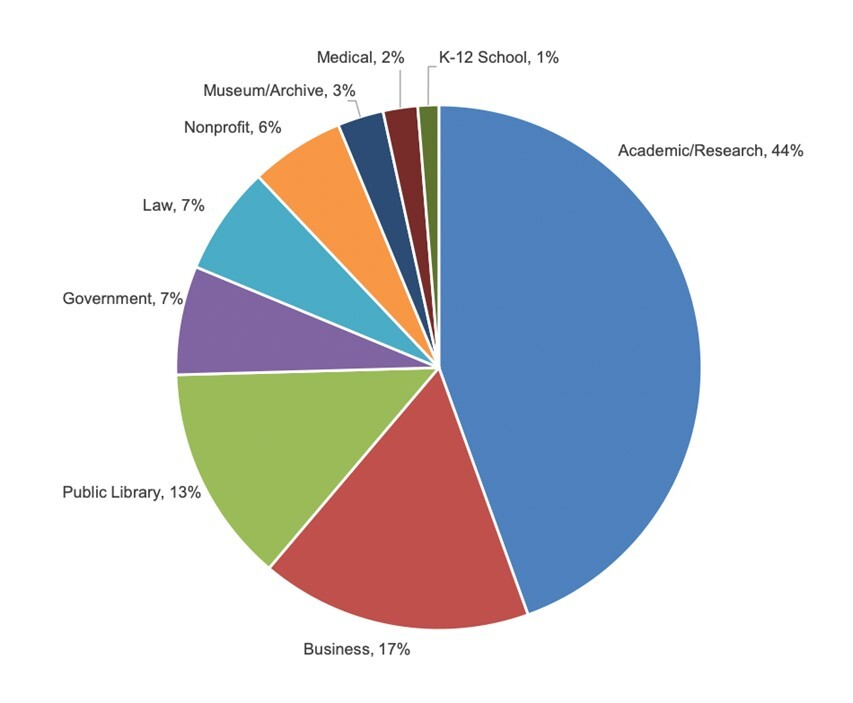
\includegraphics[keepaspectratio]{content/images/ch1-fig3.jpg}}

}

\caption{Figure 1.2 Employment sectors (San Jose State University,
2022)}

\end{figure}%

In the rest of the chapter, we look more closely at some areas where you
might work as an information professional. For each, we provide some
information on the typical jobs and the specific skills that may be
valuable, as well as other information resources such as the websites of
professional associations. We also introduce some information
professionals interviewed by Janine McGregor, a second-year MI student,
during the summer of 2022.

\section{Public libraries}\label{public-libraries}

Some job duties you might encounter while working in a public library
include programming, organizing the collection, building community
partnerships, answering information requests, providing information
literacy training, preparing library budgets and conducting needs
analyses.

Some skills that may be necessary should you wish to work in public
librarianship include supervisory experience, computer literacy,
competency with intranet content management and document management
using software, ability to work well with the public, project management
and knowledge of the trends in library service design (MLIS skills at
work). Of course, these skills are not all required, and you can learn
some on the job, but you should look to take courses and internships
that help to improve these skills.

Many professional associations to check out if you are interested in
public libraries, such as the \href{https://www.ala.org/pla/}{Public
Library Association} (a division of the
\href{https://www.ala.org/}{American Library Association}) and the
\href{https://www.nsla.ns.ca/}{Nova Scotia Library Association} (free
membership for students).

\begin{tcolorbox}[enhanced jigsaw, arc=.35mm, bottomrule=.15mm, bottomtitle=1mm, breakable, colback=white, colbacktitle=quarto-callout-tip-color!10!white, colframe=quarto-callout-tip-color-frame, coltitle=black, left=2mm, leftrule=.75mm, opacityback=0, opacitybacktitle=0.6, rightrule=.15mm, title=\textcolor{quarto-callout-tip-color}{\faLightbulb}\hspace{0.5em}{Meet a professionals}, titlerule=0mm, toprule=.15mm, toptitle=1mm]

\textbf{Dyan Bader\\
Manager\\
Systems \& Collections Access Nova Scotia Provincial Library}

As the manager of systems and collections access for the Nova Scotia
Provincial Library, Dyan works with all the public libraries outside
Halifax, which are grouped into eight regional libraries. Her team
manages the back-end systems these libraries use daily, including the
integrated library system, their discovery layer, and their digital
lending platform. Each regional library region made their own decisions
related to the integrated library system. Still, during the last five
years, Dyan and her team worked with the eight regional libraries to
integrate these into a single system called ``Same Page.'' The new
system launched in April 2022 expands access to almost 1,000,000
resources for patrons throughout Nova Scotia. With the new system,
Dyan's team must work with the different regions to ensure consensus on
all decisions that impact the system. These large projects require a lot
of planning and coordination to ensure that the best decisions are made
since they directly affect libraries across the province. Most of Dyan's
time is spent in meetings and writing documents.

The Nova Scotia Provincial Library is part of the provincial government
and supports regional libraries in several ways, either as a leader, a
partner, or a service provider. This brings a lot of variety to Dyan's
work since her projects and tasks are driven by these different roles.

Specific skills would benefit those looking to work in a similar role.
Project management is huge, as well as problem-solving, facilitation and
time management. Leadership is something that you will learn along the
way.

One piece of advice that Dyan would give to students is to focus on what
they are passionate about. For her, it was an interest in technology and
cataloging. Try your best to stick to those things, and hopefully, you
will end up in positions that allow you to explore these passions. Dyan
was lucky to have employers who supported her training goals, allowing
her to complete an advanced certificate in digital services and a
Master's certificate in project management.

Some of your first jobs can shape your career. She also suggests being
open to jobs in less urban areas as you can often gain skills in these
positions that wouldn't necessarily be possible in a more extensive
library. When you enter a larger or more structured environment, your
job description can often hem you in, and the position won't have the
flexibility that allows you to evolve quickly. Dyan's first job after
graduation was as a director of a small community college library in
Southern California. Upon starting, she soon realized that she would
need to completely replace the integrated library system and
re-catalogue the entire library. Running this massive project gave her
the experience she needed to move forward in her career and to
understand her own abilities.

\end{tcolorbox}

\begin{tcolorbox}[enhanced jigsaw, arc=.35mm, bottomrule=.15mm, bottomtitle=1mm, breakable, colback=white, colbacktitle=quarto-callout-tip-color!10!white, colframe=quarto-callout-tip-color-frame, coltitle=black, left=2mm, leftrule=.75mm, opacityback=0, opacitybacktitle=0.6, rightrule=.15mm, title=\textcolor{quarto-callout-tip-color}{\faLightbulb}\hspace{0.5em}{Meet a professional}, titlerule=0mm, toprule=.15mm, toptitle=1mm]

\textbf{Jeff Mercer\\
Deputy Chief Librarian\\
South Shore Public Libraries}\\
\strut \\
As the deputy chief librarian of a small system of libraries, Jeff is
responsible for many different things. He is in charge of PR,
promotions, community outreach, and volunteer services. He oversees all
programming at each branch, IT, and systems support or development. Jeff
also oversees policy and procedure review and revision and has some
input on collections development. In terms of staffing, Jeff deals with
hiring, performance evaluation, goal setting, training, and occasionally
scheduling.

This position has two main sides: the public side and the staff side.
Jeff's job is to say yes as much as possible to patron's requests when
working with the public. Jeff must also help his staff to be successful
in their positions.

To work in a similar role, one must have time management and people
skills. In this position, there are a lot of competing demands on your
time, such as meetings, staff support, research and workshops. People
skills can be gained through working with the public in different
service roles, such as restaurants or retail stores. It's essential to
recognize that people have different communication styles and may not
interpret what you say in the way you mean.

While you are still in school, taking advantage of student
opportunities, such as joining professional organizations, is essential.
Make sure to take any opportunity to learn from working professionals.
Jeff mentioned that specific courses within an MI degree would be
helpful for this job. Community-led services was one of them, as
responding appropriately to your community's needs is essential. He also
mentioned courses on readers' advisory since the collection goes hand in
hand with services. A library's collection needs to reflect the broader
trends in society. You want a fresh, young collection that is responsive
to people's needs.

The best advice Jeff would give is to go to any conferences, workshops
or other professional development opportunities you can. It's not just
about what you will learn but also about who you will meet and what they
can teach you. Along the way, you will gain insight that will be useful
in your future career. He also suggests that you shouldn't say no to any
opportunities. His first job gave him the skills he needed to obtain his
current job. He also believes it's important to listen if your gut tells
you that your current direction isn't right for you; you shouldn't stay
in a job you don't enjoy because you can always change direction.

\end{tcolorbox}

\section{Archives}\label{archives}

Working in archives is a common path for people taking an MI or MIM
degree. Archivists work in various organizations, including
corporations, universities, and non-profits. Some roles they may take
include archival specialist, creative arts archivist, archives project
associate or archives and special collections librarian.

While archives and libraries have many points in common, they have
significant differences that often set them apart as clearly distinct
fields. Archival records are very different than bibliographic records.
They tend to be created and maintained for different purposes and guided
by different principles and philosophies.

\begin{tcolorbox}[enhanced jigsaw, arc=.35mm, bottomrule=.15mm, bottomtitle=1mm, breakable, colback=white, colbacktitle=quarto-callout-note-color!10!white, colframe=quarto-callout-note-color-frame, coltitle=black, left=2mm, leftrule=.75mm, opacityback=0, opacitybacktitle=0.6, rightrule=.15mm, title=\textcolor{quarto-callout-note-color}{\faInfo}\hspace{0.5em}{Did you know?}, titlerule=0mm, toprule=.15mm, toptitle=1mm]

The Master of Information program offers several archives courses and an
archives
\href{https://www.dal.ca/faculty/management/school-of-information-management/current-students-site/certificates.html}{certificate}.
There are also practicum and internship opportunities available for you
to gain experience.

\end{tcolorbox}

Some job duties one may encounter working in archives include preserving
and providing access to historical records, developing an archival
digitization program, and promoting the use of collections to the
public. To get more information about the archives field, you can check
out the websites of the \href{https://archivists.ca/}{Association of
Canadian Archivists}, the \href{http://archivescanada.ca/}{Canadian
Council of Archives}, and the
\href{https://www.councilofnsarchives.ca/}{Council of Nova Scotia
Archives}.

\begin{tcolorbox}[enhanced jigsaw, arc=.35mm, bottomrule=.15mm, bottomtitle=1mm, breakable, colback=white, colbacktitle=quarto-callout-tip-color!10!white, colframe=quarto-callout-tip-color-frame, coltitle=black, left=2mm, leftrule=.75mm, opacityback=0, opacitybacktitle=0.6, rightrule=.15mm, title=\textcolor{quarto-callout-tip-color}{\faLightbulb}\hspace{0.5em}{Meet a professional}, titlerule=0mm, toprule=.15mm, toptitle=1mm]

\textbf{Sharon Murray\\
Archives Advisor\\
Council of Nova Scotia Archives}

Although Sharon does not hold an MI degree, her job is very relevant to
people within the program, and her knowledge of the profession is vast.
Before working in her current position, Sharon worked directly in the
archives, digitizing items for improved access. She systematically
processed the photographic records at the archives she worked in and
created databases to store them in. She was also required to label,
re-shelve and store items. She created web exhibits and research guides
for improved public access. Her path to archives was not a straight one.
She initially picked up archives work as a side job to improve her
research. After returning to Nova Scotia, she picked up more substantial
work in the archives. She began to pivot as she felt that the archives
were a very fulfilling fit for her skills, experiences and interests.
She found it eye-opening to see how much impact archival records can
have on the public when true, meaningful access is provided. While in
this role, she digitized several thousand photographs. She and her
colleagues had a lot of discussions about storage and access.

Sharon's current role with the Council of Nova Scotia Archives differs
significantly. The CNSA is the professional association for archives and
archivists in Nova Scotia. The organization's purpose is to provide
support, education and advocacy for those in the profession. In Nova
Scotia, there are around 75 archives that are members, which range
vastly in size and resources from small volunteer-run archives to larger
ones with multiple permanent paid staff. The CNSA offers courses,
workshops and training opportunities to help members develop the
essential knowledge and skills to manage their archives. Sharon teaches
most courses, with 50\% of her role offering advisory services. Due to
this, she must keep on top of the current discussions and needs within
the profession to ensure that the knowledge she is conveying is current.

Sharon describes the two most essential skills in the archives
profession as a background in Equity Diversity and Inclusion (EDI) and
digital preservation and access knowledge. The profession is currently
at a turning point in which they acknowledge their role in silencing the
stories and voices of Indigenous peoples in Canada. Archivists want to
ensure that they are doing the right thing in the future by endeavouring
to preserve records, stories and information about all people. The
second turning point she described was the digital turn. Archives are
heading into brave new territory where it isn't paper-based records but
digital content that must be preserved. A lot more digital-born content
will require digital infrastructure to be built. It is also essential
for archivists to have relational skills, meaning a desire to build
relationships and connect communities. Archive work is becoming more
service-oriented.

The best advice that Sharon would give to students is to build
relationships with people working in the field, as it will help them to
understand the realities of the profession. It will also help you
understand what you have to offer and how your skills and strengths
might be helpful to the community. She also suggests looking outside
Halifax for summer work positions, as many of these small organizations
seek help. You will get the opportunity to work on many aspects of the
archive and likely learn a lot about community building.

\end{tcolorbox}

\section{Museums}\label{museums}

Museums also often have libraries and archives that can be open to the
public (increasingly so, with collections being digitized and made
available on the web). Depending on the type of museum, these libraries
and archives can be part of the collections or exist to support the
museum's activities. For example, a good exhibit might rely on having
done research on the topic and its social or historical context or on
specific items that are part of the exhibit. Then, you can think of
museums as just another type of organization where librarians or
archivists are needed.

Another critical role for information professionals in museums involves
dealing with information systems and users. Museums increasingly have
online collections and databases to support them. These require a set of
competencies and skills, such as database management, organization of
information, and user-centred web design, that you can develop during
your MI degree.

More generally, the close relationship between the information and
museum fields may be blurry enough that your information degree could
help you compete for any museum role, especially if you have a
background in the arts and humanities or another area that is relevant
to a particular museum.

To better understand the jobs available in the museum space, check out
the Canadian Museums Association (\url{https://museums.ca/}) and their
\href{https://museums.ca/site/aboutthecma/careersheritageycw/jobsinheritage}{job
board}.

\section{Academic libraries}\label{academic-libraries}

There are many different roles that one can have within an academic
library. These include but are not limited to access and reference
services librarian, outreach and diversity librarian, materials and
image librarian, and staff engagement liaison. Some key service roles
include reference assistance, assisting faculty in research and teaching
research, delivering courses on research, creating LibGuides, helping to
select which journals to purchase, analyzing usage statistics and
outreach and marketing.

The Dalhousie Libraries website may be an excellent place to explore if
you are interested in academic libraries. You probably used a similar
website before to search for resources, but checking out the services
and about us pages might help you grasp the broad range of services that
academic libraries offer. You should also check out the
\href{https://www.carl-abrc.ca/}{Canadian Association of Research
Libraries} (CARL) and the \href{https://capalibrarians.org}{Canadian
Association of Professional Academic Librarians} (CAPAL)

\section{Law librarianship}\label{law-librarianship}

An information manager may have many different job titles when working
in law. Examples of these include law practice and technology librarian
and instructional law librarian. Some people choose to acquire a law
degree along with their information degree to further their skills. Some
job duties you may have working in legal librarianship include assisting
the law community in finding and evaluating information, developing
instructional programs on legal technologies, teaching law courses, and
monitoring vendor communication for new titles.

Common skills employers search for in legal librarianship include
exceptional client service, discretion when dealing with confidential
information, knowledge of online legal research platforms, experience
working on projects related to digitization, project management and
teaching. You can tailor your courses to these skills while in school
and find ways to use what you have learned in your interviews upon
graduation (MLIS skills at work, 2022).

\begin{tcolorbox}[enhanced jigsaw, arc=.35mm, bottomrule=.15mm, bottomtitle=1mm, breakable, colback=white, colbacktitle=quarto-callout-note-color!10!white, colframe=quarto-callout-note-color-frame, coltitle=black, left=2mm, leftrule=.75mm, opacityback=0, opacitybacktitle=0.6, rightrule=.15mm, title=\textcolor{quarto-callout-note-color}{\faInfo}\hspace{0.5em}{Did you know?}, titlerule=0mm, toprule=.15mm, toptitle=1mm]

One of the MI electives is a course on legal librarianship (INFO6320
Legal Literature and Librarianship), part of the Librarianship
\href{https://www.dal.ca/faculty/management/school-of-information-management/current-students-site/certificates.html\#librarianship}{Certificate}.

\end{tcolorbox}

\section{Health librarianship}\label{health-librarianship}

Your information management degree can lead to various careers in the
health sector, with job titles such as medical content reference
librarian, medical research librarian, or health sciences librarian.
Check out the websites of the \href{https://www.chla-absc.ca/}{Canadian
Health Libraries Association} and the
\href{https://www.mlanet.org/}{Medical Library Association} for more
insights into that area of the field.

Health and law librarianship are sometimes put into the broader
\textbf{special libraries} category alongside most libraries operating
in highly specialized public, non-profit and corporate settings. You
might be surprised about the number of libraries and librarians
(sometimes under different labels) found in various organizations, such
as the \href{https://www.asc-csa.gc.ca/eng/library/}{Canadian Space
Agency}, the Cirque du Soleil, or the Montreal Botanical Garden. Check
out the Canadian chapter of the Special Library Association (SLA) to
learn more about special libraries.

\begin{tcolorbox}[enhanced jigsaw, arc=.35mm, bottomrule=.15mm, bottomtitle=1mm, breakable, colback=white, colbacktitle=quarto-callout-caution-color!10!white, colframe=quarto-callout-caution-color-frame, coltitle=black, left=2mm, leftrule=.75mm, opacityback=0, opacitybacktitle=0.6, rightrule=.15mm, title=\textcolor{quarto-callout-caution-color}{\faFire}\hspace{0.5em}{Beware}, titlerule=0mm, toprule=.15mm, toptitle=1mm]

While we use the terms librarian and libraries a lot, it's essential to
know that your degree will open doors to the health sector in libraries
and all kinds of data or information management roles. This is true for
all sectors discussed in this chapter.

\end{tcolorbox}

\section{Data management and data
science}\label{data-management-and-data-science}

There are many different \textbf{jobs} in the data management field.
Some job titles include data analytics manager, data librarian, data
visualization and GIS specialist, and data governance manager. Some
duties you may encounter within these roles include leading a university
library's research data services initiative, partnering with researchers
to advance the knowledge and management of data, or answering questions
on data management for faculty and staff at a university (MLIS skills at
work, 2022).

If you are passionate or curious about data, consider tailoring your
courses to working with data. Courses such as data science and data
management will help you to learn the skills you need to succeed.

With the world shifting towards more online content, digitization is
becoming increasingly important, making digital librarianship an
increasingly relevant area of specialization. Job titles in this area
include digital collections manager, electronic resources librarian,
virtual resources librarian or digital and automated services librarian.
Typical roles include supervising activities related to digitizing
collections, providing consultation and technical support for developing
technology-related research projects or engaging in the assessment,
maintenance and enhancement of digital collections and services.

If you are interested in digital librarianship, taking extra advanced
technology courses during your degree could be helpful. This will help
you to gain valuable skills such as the ability to learn new
technologies quickly, experience with metadata, knowledge of
digitization standards and an interest in electronic information sources
and organizations.

\begin{tcolorbox}[enhanced jigsaw, arc=.35mm, bottomrule=.15mm, bottomtitle=1mm, breakable, colback=white, colbacktitle=quarto-callout-tip-color!10!white, colframe=quarto-callout-tip-color-frame, coltitle=black, left=2mm, leftrule=.75mm, opacityback=0, opacitybacktitle=0.6, rightrule=.15mm, title=\textcolor{quarto-callout-tip-color}{\faLightbulb}\hspace{0.5em}{Meet a professional}, titlerule=0mm, toprule=.15mm, toptitle=1mm]

\textbf{Stephanie Bilodeau\\
Manager, Open Government and Data Governance\\
Royal Canadian Mounted Police -- IM/IT Program}

Stephanie wears two hats with her job at the RCMP; she is the manager of
Open Government and Data Governance. There is a significant need for
these positions because programmers created systems to store data, but
more needs to be done to organize and manage that data. They have found
that when using these systems, things aren't accurate, and queries are
not constantly pulling up the right data. There is also bias in the
systems depending on who entered the data. Some systems have too much
data as it hasn't been managed, disposed of or cleaned in years,
creating privacy issues. This is where data governance comes into play.
It is Stephanie's job to govern how the data is entered, how the data is
utilized and how it is managed.

Stephanie provides service to clients. Her department serves all the
department employees, helping them organize, collect, store, preserve,
secure and dispose of information. She also must write policy
instruments, including standards, guidelines, procedures, and processes
for managing information. She must establish governance and facilitate
decision-making with those with authority and responsibility regarding
the data and information. As a manager, Stephanie manages the office,
the employees, the workload, the scheduling of work, and the delegation
of work. Open government is concerned with publishing information that
would be in the public interest to be transparent. There is a lot of
work to do in this regard, including ensuring that information is
protected and publishing relevant information. To enhance democracy, all
citizens should be able to participate in these discussions.

If you want to work in a similar position, you must be a people person.
The job requires you to meet with clients, partners and collaborators
and to work with people to help enhance their experience of working with
information. This is a position in which you would rarely work alone. It
would be best if you were organized and technologically savvy. This
position is incredibly tech-focused, so knowing how information is
managed through IT systems is essential. You must be adaptable as the
role changes and open-minded to different cultures, languages, and
personalities. You must also be bilingual, speaking both French and
English.

The Federal Student Work Experience Program is a database for hiring
students through the Government of Canada. Stephanie suggests you put
your resume in as you may be hired for a government position. They offer
full-time positions during the summer with flexible hours during the
school year. They also can bridge students into permanent positions
after they graduate.\\
https://www.canada.ca/en/treasury-board-secretariat/services/pay/rates-pay/student-employment-programs-federal-government/federal-student-work-experience-program.html

The best advice Stephanie would give is to be open-minded and willing to
learn constantly. Always try new things and make sure that the work you
are doing is aligned with your organization's mission and corporate
vision.

\end{tcolorbox}

\section{Knowledge management}\label{knowledge-management}

Knowledge managers can work in various sectors, including non-profits,
government or corporations. Some roles that fall under knowledge
management include knowledge synthesizer, knowledge analyst, knowledge
navigator and, of course, knowledge manager. Some of the primary duties
you may encounter within this field are handling a company's knowledge
management operations, formulating a knowledge management strategy,
managing knowledge management staff and influencing organizational
change. Tasks you may be asked to perform include curating technical
website content, designing and implementing practical learning
activities and managing knowledge-sharing events.

\begin{tcolorbox}[enhanced jigsaw, arc=.35mm, bottomrule=.15mm, bottomtitle=1mm, breakable, colback=white, colbacktitle=quarto-callout-tip-color!10!white, colframe=quarto-callout-tip-color-frame, coltitle=black, left=2mm, leftrule=.75mm, opacityback=0, opacitybacktitle=0.6, rightrule=.15mm, title=\textcolor{quarto-callout-tip-color}{\faLightbulb}\hspace{0.5em}{Meet a professional}, titlerule=0mm, toprule=.15mm, toptitle=1mm]

\textbf{Trecia\\
Community Services Librarian and Managing Branch Librarian of the
Stellarton and Trenton Public Libraries and the regional Borrow-by-Mail
service.}

Trecia enrolled in the MLIS program at McGill University and specialized
in Knowledge Management to learn how to share knowledge best. During the
final term of her program, she completed an internship with Rio Tinto
Alcan in their International Intellectual Properties Division, and
there, she learned that effective knowledge-gathering and sharing
strategies rely on a sound understanding of your audiences. Knowledge
Management work often involves doing research to fulfill specific needs
and constantly re-evaluating knowledge purpose and use to ensure that
the collected resources are of value for the people in the organization
using them.

Trecia is now the Community Services Librarian and Managing Branch
Librarian of the Stellarton and Trenton Public Libraries and the
regional Borrow-by-Mail service. In addition, her job portfolio covers
the regional areas of responsibility for Public Relations and
Communications, Programming, Outreach, and Services for Adults. One of
her main focuses is developing Community-based programs and services,
which involves working with the staff in each location to plan
programming responsive to their communities' needs. She finds that
programming works best when there is engagement with the community to
participate. Community-led programming begins with conversations with
the community-at-large and other community service providers to
determine programs and services of interest and value. This is the key
to building responsive public library services.

According to Trecia, some essential skills required of successful public
librarians and public library staff include communication and
leadership. Communication is critically important, mainly formal
communication skills such as being comfortable with public speaking
(giving presentations and leading workshops), understanding the evolving
social media etiquette, and crafting effective media releases and grant
applications (and reports). Management, leadership skills, and solid
project management experience are vital to creating a healthy,
responsive, thriving workplace environment.

To set yourself up for success in this field during your degree, Trecia
suggests looking into how the interests of the faculty members in your
program may align with yours. This can lead to research work
opportunities. She also recommends considering how your background and
experiences can be mobilized into your career in information - the
strengths you can bring forward and how the information degree will
complement these strengths. The information field is broad and offers
many opportunities, so Trecia suggests that you try to take on projects
that are meaningful and that you can connect to your interests.

\end{tcolorbox}

\section{Information as a research
field}\label{information-as-a-research-field}

The information field is not just a diverse set of competencies and
career pathways. It is also a research discipline with peer-reviewed
journals, scholarly societies, and conferences. The field has many names
that have grown or declined in popularity, such as library science,
library studies, information science, information studies, library and
information science. As Figure 1 at the beginning of the chapter
highlighted, the field is also not a monolith; it comprises a wide range
of research areas from arts and humanities to natural sciences. If you
were to retrieve all the Library and Information Science research in the
Web of Science and visualize it in a citation network, it would probably
look like this figure:

\begin{figure}[H]

{\centering \pandocbounded{\includesvg[keepaspectratio]{content/images/CC_DC with manual labels_title.svg}}

}

\caption{Figure 1.3. map of Canadian LIS publications (Mongeon et al.
2023).}

\end{figure}%

\begin{tcolorbox}[enhanced jigsaw, arc=.35mm, bottomrule=.15mm, bottomtitle=1mm, breakable, colback=white, colbacktitle=quarto-callout-note-color!10!white, colframe=quarto-callout-note-color-frame, coltitle=black, left=2mm, leftrule=.75mm, opacityback=0, opacitybacktitle=0.6, rightrule=.15mm, title=\textcolor{quarto-callout-note-color}{\faInfo}\hspace{0.5em}{Did you know?}, titlerule=0mm, toprule=.15mm, toptitle=1mm]

If you want to learn how to analyze research fields and produce
visualizations like Figure 1.3, consider taking the Bibliometrics and
Scholarly Communications course (INFO6550)..

\end{tcolorbox}

If you want to know more about research in the field, check out the
profiles of
\href{https://www.dal.ca/faculty/management/faculty-staff/information-science.html}{faculty
members of the Department of Information Science} and get in touch with
them to know more about their research. You can also look at this
\href{https://www.zotero.org/groups/sim_research/library/}{bibliography
of all the research authored or co-authored by someone at the Department
of Information Science}. You can also discuss it with your academic
advisor or check out the \href{https://cais-acsi.ca/}{Canadian
Association for Information Science (CAIS)}, or the
\href{https://www.asist.org/}{Association for Information Science and
Technology (ASIST)}.

\begin{tcolorbox}[enhanced jigsaw, arc=.35mm, bottomrule=.15mm, bottomtitle=1mm, breakable, colback=white, colbacktitle=quarto-callout-tip-color!10!white, colframe=quarto-callout-tip-color-frame, coltitle=black, left=2mm, leftrule=.75mm, opacityback=0, opacitybacktitle=0.6, rightrule=.15mm, title=\textcolor{quarto-callout-tip-color}{\faLightbulb}\hspace{0.5em}{Did you know?}, titlerule=0mm, toprule=.15mm, toptitle=1mm]

Because the Department of Information Science is an institutional member
of the Canadian Association for Information Science, you can become a
member for free. You can register here:
\url{https://cais-acsi.ca/membership}.

\end{tcolorbox}

\section{Conclusion}\label{conclusion}

This chapter aimed to give students an overview of the information field
by presenting some of the critical sectors and positions that graduates
from ours and similar programs are likely to occupy in their careers. If
you think, ``But the area that I'm most interested in wasn't discussed
here. Am I in the wrong program?'' do not worry. It's most likely due to
the non-exhaustive nature of this overview. Of course, you can always
contact the instructor, your academic advisor, or the program
coordinator if you have questions or concerns regarding your learning
and professional goals.

\section{Self-reflection questions}\label{self-reflection-questions}

\begin{itemize}
\tightlist
\item
  What are the sectors or types of information work interest you the
  most?
\item
  What are the primary skills or knowledge you will develop during the
  program?
\end{itemize}

You may have a clear idea of the answer to that question, but you may
also feel like you don't know enough at this point. Perfect, that's what
this entire course and program are for. The Department of Information
faculty and staff are here to guide you and help you make the best of
your program and what will come next.

\section{References}\label{references}

\bookmarksetup{startatroot}

\chapter{What is Information?}\label{what-is-information}

\section{Learning objectives}\label{learning-objectives-1}

So what is information anyway? If we call ourselves information
managers, specialists, information professionals, or information
scientists. In that case, it seems appropriate to seek a clear
understanding of what we are experts in. This chapter aims to explore
the concept of information and its related concepts as they have been
discussed within the library and information science field. By the end
of this chapter, you should be able to:

\begin{itemize}
\tightlist
\item
  Recognize the challenges in defining the concept of information.
\item
  Name and explain some of the concepts related to information.
\item
  Situate these concepts in relationship with each other.
\end{itemize}

\begin{tcolorbox}[enhanced jigsaw, arc=.35mm, bottomrule=.15mm, bottomtitle=1mm, breakable, colback=white, colbacktitle=quarto-callout-note-color!10!white, colframe=quarto-callout-note-color-frame, coltitle=black, left=2mm, leftrule=.75mm, opacityback=0, opacitybacktitle=0.6, rightrule=.15mm, title=\textcolor{quarto-callout-note-color}{\faInfo}\hspace{0.5em}{Clarification}, titlerule=0mm, toprule=.15mm, toptitle=1mm]

The goal is not for you to come out of this week with a final definition
of information but to TRY to define it and to position the concept in
relation to other concepts so that you have, at the very least, an
understanding of the various (sometimes conflicting) ways of thinking
about information, and possibly a start of a conceptual framework that
you will keep expanding as you progress in the MI program.

\end{tcolorbox}

\section{What is information?}\label{what-is-information-1}

\begin{tcolorbox}[enhanced jigsaw, arc=.35mm, bottomrule=.15mm, bottomtitle=1mm, breakable, colback=white, colbacktitle=quarto-callout-tip-color!10!white, colframe=quarto-callout-tip-color-frame, coltitle=black, left=2mm, leftrule=.75mm, opacityback=0, opacitybacktitle=0.6, rightrule=.15mm, title=\textcolor{quarto-callout-tip-color}{\faLightbulb}\hspace{0.5em}{Tip}, titlerule=0mm, toprule=.15mm, toptitle=1mm]

Think of the word information, and write down the first ten words (no
more) that come to your mind.

\begin{itemize}
\item
  Was it difficult?
\item
  In what way are your words related to one another beyond their common
  relationship to the word information?
\end{itemize}

\end{tcolorbox}

Now that we have brought the concept of information to our attention let
us do what we were all taught (at least in my generation) to do when
seeking to understand the meaning of a term and turn to a dictionary to
obtain a definition of the term ``information''. Here are the
definitions offered by the Merriam-Webster Dictionary:

\begin{enumerate}
\def\labelenumi{\arabic{enumi}.}
\tightlist
\item
  Knowledge obtained from investigation, study, or instruction
\item
  Intelligence, News
\item
  Facts, data
\item
  The attribute inherent in and communicated by one of two or more
  alternative sequences or arrangements of something (such as
  nucleotides in DNA or binary digits in a computer program) that
  produce specific effects
\item
  A signal or character (as in a communication system or computer)
  representing data
\item
  Something (such as a message, experimental data, or a picture) that
  justifies a change in a construct (such as a plan or theory) that
  represents physical or mental experience or another construct
\item
  A quantitative measure of the content of information. Specifically: a
  numerical quantity that measures the uncertainty in the outcome of an
  experiment to be performed
\item
  The communication or reception of knowledge or intelligence
\item
  The act of informing against a person
\item
  A formal accusation of a crime made by a prosecuting officer as
  distinguished from an indictment presented by a grand jury
\end{enumerate}

\begin{tcolorbox}[enhanced jigsaw, arc=.35mm, bottomrule=.15mm, bottomtitle=1mm, breakable, colback=white, colbacktitle=quarto-callout-tip-color!10!white, colframe=quarto-callout-tip-color-frame, coltitle=black, left=2mm, leftrule=.75mm, opacityback=0, opacitybacktitle=0.6, rightrule=.15mm, title=\textcolor{quarto-callout-tip-color}{\faLightbulb}\hspace{0.5em}{Stop and reflect}, titlerule=0mm, toprule=.15mm, toptitle=1mm]

Think of the ten words you came up with earlier.

\begin{itemize}
\item
  To which of the ten definitions above are your ten words most strongly
  related?
\item
  Which of the ten definitions do you think are relevant to our field?
  Which do you think are not?
\end{itemize}

\end{tcolorbox}

\section{Situating information in its disciplinary
contexts}\label{situating-information-in-its-disciplinary-contexts}

One of the things that you may have noticed with the dictionary
definitions is that some of them are unrelated to the information
professions as you may now think of them. Indeed, one of the main issues
with the word ``information'' is that it is used in a wide variety of
contexts or disciplines, and the meaning of the word often depends on
that context or discipline. What, then, would be the specific
understanding of information that is most useful for information
management? The figure below is a network showing the links between
disciplines represented by a large circle and the most frequent keywords
containing the word ``information'' that research publications in these
disciplines contain. The orange circle represents our field labelled
``LIS'' (for Library and Information Science).

\pandocbounded{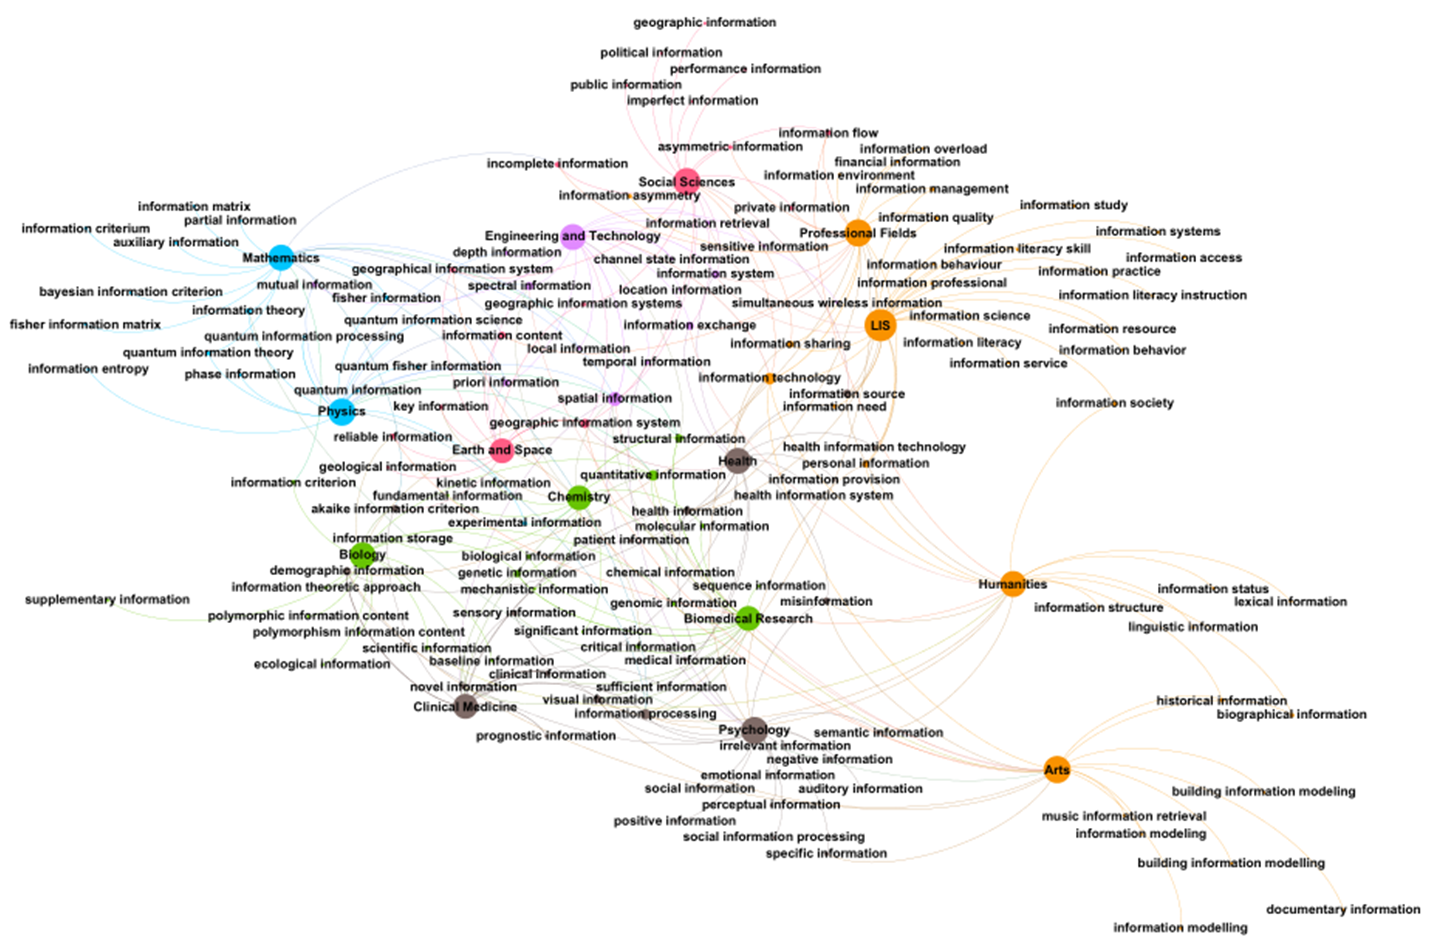
\includegraphics[keepaspectratio]{content/images/paste-E85F17EB.png}}

\begin{tcolorbox}[enhanced jigsaw, arc=.35mm, bottomrule=.15mm, bottomtitle=1mm, breakable, colback=white, colbacktitle=quarto-callout-tip-color!10!white, colframe=quarto-callout-tip-color-frame, coltitle=black, left=2mm, leftrule=.75mm, opacityback=0, opacitybacktitle=0.6, rightrule=.15mm, title=\textcolor{quarto-callout-tip-color}{\faLightbulb}\hspace{0.5em}{Stop and reflect}, titlerule=0mm, toprule=.15mm, toptitle=1mm]

\begin{itemize}
\item
  What did you think of this map? Were you able to observe apparent
  disciplinary differences in the uses of the term ``information''?
\item
  Did the terms linked to the LIS field make sense to you based on your
  knowledge of the field? Were some of them surprising?
\end{itemize}

\end{tcolorbox}

\section{A definition of information for the information
field?}\label{a-definition-of-information-for-the-information-field}

Whatever name the schools or programs that train information
professionals are called (e.g., Information Management, Information
Studies, Information Science), most have in common that one word:
``information''. It is thus no surprise that at least a handful of
scholars working in these schools or departments have sought to provide
some conceptual clarity regarding that word that unites us all. What may
be more surprising, however, is that several decades of scholarship and
debates have not achieved consensus on the definition of the word
information. Still, these conceptual explorations have generated many
attempts at such a definition, leading us to explore a range of other
correlated concepts that have sometimes been used to determine what is
(and what is not) information. They have also generated entertaining
debates, such as the well-known discussion between Birger Hjørland and
Marcia Bates on whether understanding information as an objective
phenomenon is helpful for the field. In the next section, we provide an
overview of how three scholars of the information disciplines have
proposed that we should think about the term information: Marcia Bates,
Birger Hjørland, and Michael Buckland.

\subsection{Bates: Fundamental forms of
information}\label{bates-fundamental-forms-of-information}

Marcia Bates believed that all information is natural and exists in the
material world of matter and energy and that ``almost anything existing
in the universe that can come into human and other animals' purview can
be experienced as information'' (Bates 2006, 1033). From there, she
constructed a glossary of the different forms of information:

\begin{itemize}
\item
  \textbf{Embedded information}: Information left behind on earth by
  animals. Includes such things as human-created tools or paths through
  the woods.
\item
  \textbf{Embodied} \textbf{information}: The corporeal expression or
  manifestation of information previously in encoded form.
\item
  \textbf{Encoded} \textbf{information}: Natural information organized
  symbolically, linguistically, or signal-based.
\item
  \textbf{Enacted information}: The pattern of organization of actions
  of an animal in, and interacting with, its environment, utilizing
  capabilities and experience from its neural stores.
\item
  \textbf{Experienced information}: The pattern of organization of
  subjective experience, the feeling of being in life, of an animal.
\item
  \textbf{Exosomatic} \textbf{information}: Information that is stored
  outside of the body.
\item
  \textbf{Expressed} \textbf{information}: The pattern of organization
  of communicatory scents, calls, gestures, and ultimately, the human
  spoken language used to communicate among species members and between
  species.
\item
  \textbf{Genetic information}: Information contained in the genotype
\item
  \textbf{Genotype}: The genetic constitution of a living thing.
\item
  \textbf{Information 1}: The pattern of organization of matter and
  energy
\item
  \textbf{Information 2}: Some pattern of organization of matter and
  energy to which a living being has given meaning.
\item
  \textbf{Knowledge}: Information that has been integrated with other
  contents of understanding and, therefore, given meaning.
\item
  \textbf{Neural-cultural information}: Information created by,
  processed in, or disseminated from animal nervous systems, especially
  human nervous systems. (Neural information may also be used for lower
  animals and/or specifically for the nervous system structures that
  make memory and action possible in general in animals and humans.)
\item
  \textbf{Phenotype}: The genetically and environmentally determined
  embodiment of a genotype.
\item
  \textbf{Recorded} \textbf{information}: Information that has been
  stored in a durable medium.
\item
  \textbf{Represented information}: Natural information that is encoded
  or embodied.
\item
  \textbf{Trace} \textbf{information}: The information that remains
  after a species is done with it. For example, a no-longer-used wasps'
  nest.
\end{itemize}

\begin{tcolorbox}[enhanced jigsaw, arc=.35mm, bottomrule=.15mm, bottomtitle=1mm, breakable, colback=white, colbacktitle=quarto-callout-note-color!10!white, colframe=quarto-callout-note-color-frame, coltitle=black, left=2mm, leftrule=.75mm, opacityback=0, opacitybacktitle=0.6, rightrule=.15mm, title=\textcolor{quarto-callout-note-color}{\faInfo}\hspace{0.5em}{Suggested reading}, titlerule=0mm, toprule=.15mm, toptitle=1mm]

If you want to read more about the fundamental forms of information and
their relevance for the information field, according to Marcia Bates,
you can read the full article:

Bates, Marcia J. 2006. ``Fundamental Forms of Information.''
\emph{Journal of the American Society for Information Science and
Technology} 57 (8): 10331045. \url{https://doi.org/10.1002/asi.20369}.

\end{tcolorbox}

\subsection{Hjørland: Information as a subjective/situation
construct?}\label{hjuxf8rland-information-as-a-subjectivesituation-construct}

According to Hjørland (2007), there are two basic views of information:

\begin{itemize}
\item
  \textbf{Objective information}: any difference (in patterns of matter
  and energy, as in Bates' concept of information 1).
\item
  \textbf{Subjective/situational information}: a difference that makes a
  difference.
\end{itemize}

In his paper, @hjorland\_information\_2007 criticizes Bates' fundamental
form of information and argues that only subjective information is
relevant to the field. While Bates' concept of information 2 is
compatible with that view, the concept of information 1 is not and
should be ignored. Hjørland also argues that Bates' definition of
information 2 is too limited because it specifies the need for a living
being to interpret the signal and give it meaning, which excludes the
idea of computers processing information.

\begin{tcolorbox}[enhanced jigsaw, arc=.35mm, bottomrule=.15mm, bottomtitle=1mm, breakable, colback=white, colbacktitle=quarto-callout-tip-color!10!white, colframe=quarto-callout-tip-color-frame, coltitle=black, left=2mm, leftrule=.75mm, opacityback=0, opacitybacktitle=0.6, rightrule=.15mm, title=\textcolor{quarto-callout-tip-color}{\faLightbulb}\hspace{0.5em}{Stop and reflect}, titlerule=0mm, toprule=.15mm, toptitle=1mm]

\begin{itemize}
\tightlist
\item
  Do you agree with Hjørland and think computers can give meaning to the
  signal they process?
\end{itemize}

\end{tcolorbox}

For Hjørland, If no one is aware of an object, then it cannot be
information; it can become information once someone (or a computer)
becomes aware of it. Under the situational definition of information,
whether or not something is information depends on the circumstances
surrounding the document, data, object or event. These things may be
defined as information in certain situations but not others. This idea
becomes complicated when you think of how vast the range of information
can be; determining if and how something can be informative is very
difficult. A tree can be informative in multiple ways. It will represent
other trees of its kind, but the rings inside the trunk also provide
information about weather patterns. Anything can then be information
given the proper context. Hence, for Hjørland, there is no point in ever
considering information as an objective phenomenon without any context
since information is determined and defined by that context.

\begin{tcolorbox}[enhanced jigsaw, arc=.35mm, bottomrule=.15mm, bottomtitle=1mm, breakable, colback=white, colbacktitle=quarto-callout-note-color!10!white, colframe=quarto-callout-note-color-frame, coltitle=black, left=2mm, leftrule=.75mm, opacityback=0, opacitybacktitle=0.6, rightrule=.15mm, title=\textcolor{quarto-callout-note-color}{\faInfo}\hspace{0.5em}{Suggested readings}, titlerule=0mm, toprule=.15mm, toptitle=1mm]

If you want to read more about Hjørland's view of information and his
argument against Bates' information 1 concept, you can read the full
article:

Hjørland, Birger. 2007. ``Information: Objective or
Subjective/Situational?'' \emph{Journal of the American Society for
Information Science and Technology} 58 (10): 1448--56.
\url{https://doi.org/10.1002/asi.20620}.

This article was followed by a response from Bates, followed by another
response from Hjørland if you are curious to see how this little dispute
unfolded.

Bates, M. J. (2008). Hjørland's critique of Bates' work on defining
information. \emph{Journal of the American Society for Information
Science and Technology}, \emph{59}(5), 842--844.
\url{https://doi.org/10.1002/asi.20796}

Hjørland, B. (2009). The controversy over the concept of
``information'': A rejoinder to Professor Bates. \emph{Journal of the
American Society for Information Science and Technology}, \emph{60}(3),
643--643. \url{https://doi.org/10.1002/asi.20972}

\end{tcolorbox}

\subsection{Buckland: information as thing, process, and
knowledge}\label{buckland-information-as-thing-process-and-knowledge}

Buckland (1991) describes information in three ways;
information-as-thing, information-as-process, and
information-as-knowledge.

Information can be considered a \textbf{thing} when it describes an
object, such as data or documents. They are considered information
because they are informative; they impart knowledge or communicate
information. Everything around you can be informative, which is
problematic for information professionals. Indeed, the information
systems we manage deal directly with information-as-thing and since we
cannot deal with everything in the world, we need to decide what kinds
of information-as-thing we choose to engage with. The term document may
be helpful here. According to Briet (1951), a document is ``any physical
or symbolic sign, preserved or recorded, intended to represent,
reconstruct, or demonstrate a physical or conceptual phenomenon''. She
is well known for her example of an antelope as a document. She
discusses how an antelope living free in Africa would not be considered
a document, but once captured and put into a zoo, it becomes an object
of study. At that point, it has become a document as it is now physical
evidence to be used by researchers. Information as a \textbf{process}
occurs when someone is informed of something, changing what they know,
and what is known is \textbf{information-as-knowledge} that exists in an
intangible form in the mind of the knowing entity and cannot be observed
or measured.

\begin{tcolorbox}[enhanced jigsaw, arc=.35mm, bottomrule=.15mm, bottomtitle=1mm, breakable, colback=white, colbacktitle=quarto-callout-tip-color!10!white, colframe=quarto-callout-tip-color-frame, coltitle=black, left=2mm, leftrule=.75mm, opacityback=0, opacitybacktitle=0.6, rightrule=.15mm, title=\textcolor{quarto-callout-tip-color}{\faLightbulb}\hspace{0.5em}{Stop and reflect}, titlerule=0mm, toprule=.15mm, toptitle=1mm]

\begin{itemize}
\tightlist
\item
  One branch of our field is called knowledge management. If knowledge
  is information in an intangible form that cannot be observed or
  measured, how can it be managed?
\end{itemize}

\end{tcolorbox}

\begin{tcolorbox}[enhanced jigsaw, arc=.35mm, bottomrule=.15mm, bottomtitle=1mm, breakable, colback=white, colbacktitle=quarto-callout-note-color!10!white, colframe=quarto-callout-note-color-frame, coltitle=black, left=2mm, leftrule=.75mm, opacityback=0, opacitybacktitle=0.6, rightrule=.15mm, title=\textcolor{quarto-callout-note-color}{\faInfo}\hspace{0.5em}{Suggested reading}, titlerule=0mm, toprule=.15mm, toptitle=1mm]

To read more about Buckland's concepts of information-as-thing,
information-as-process, and information-as-knowledge, you can read the
full article if you haven't already:

Buckland, M. K. (1991). Information as thing. \emph{Journal of the
American Society for Information Science}, \emph{42}(5), 351--360.
\url{https://doi.org/10.1002/(SICI)1097-4571(199106)42:5\%3C351::AID-ASI5\%3E3.0.CO;2-3}

\end{tcolorbox}

\section{The data, information, knowledge, and wisdom
pyramid}\label{the-data-information-knowledge-and-wisdom-pyramid}

In exploring the concept of information, we came across many other
terms, such as document, knowledge, understanding, and data. One way to
try to make sense of it is by situating each of these terms in relation
to each other. The data, information, knowledge and wisdom (DIKW)
hierarchy or pyramid (pictured below) was not developed by scholars in
the LIS field. Still, it can be helpful to us as it offers a visual
representation of the relationship between some of the terms we
encountered so far.

\begin{figure}[H]

{\centering \pandocbounded{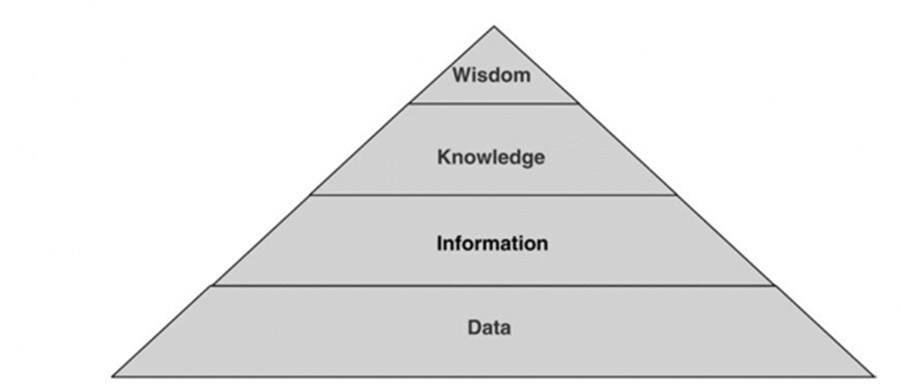
\includegraphics[keepaspectratio]{content/images/ch2-dikw-pyramid.jpg}}

}

\caption{Figure 2. The data, information, knowledge and wisdom (DIKW)
pyramid}

\end{figure}%

Many authors agree that the first appearance of the hierarchy was in
T.S. Elliot's poem The Rock.

\begin{quote}
``Where is the wisdom that we have lost in knowledge?

Where is the knowledge that we have lost in information?''
\end{quote}

The hierarchy connects wisdom, knowledge, information, and data to
identify how entities at the higher levels are created from those at
lower levels. According to the pyramid, data generates information,
information generates knowledge, and knowledge generates wisdom.
However, just as defining information has proven quite challenging,
there is no consensus on the definition of each level of the pyramid, no
consensus regarding the number of layers the pyramid should have, and no
consensus regarding the hierarchical nature of the relationship between
the concepts. (Rowley 2007).

Rowley (2007) reviewed the literature on the pyramid and how each
concept was defined. She found that most definitions of data point to it
being discrete objects, facts or observations, or recorded descriptions
of things, events, activities, or transactions. According to Rowley's
review, researchers describe information as data formatted, processed,
used, or given meaning. Knowledge is often defined as information
processed in an individual's mind and may also include the requirement
that this process has generated justified and true beliefs about the
world (Rowley 2007).

\begin{tcolorbox}[enhanced jigsaw, arc=.35mm, bottomrule=.15mm, bottomtitle=1mm, breakable, colback=white, colbacktitle=quarto-callout-tip-color!10!white, colframe=quarto-callout-tip-color-frame, coltitle=black, left=2mm, leftrule=.75mm, opacityback=0, opacitybacktitle=0.6, rightrule=.15mm, title=\textcolor{quarto-callout-tip-color}{\faLightbulb}\hspace{0.5em}{Stop and reflect}, titlerule=0mm, toprule=.15mm, toptitle=1mm]

\begin{itemize}
\item
  If, according to the pyramid, information is processed data, and
  knowledge is processed information, then how would you define wisdom?
\item
  Does good data necessarily lead to good information?
\item
  In what ways do information professionals deal with each level of the
  pyramid?
\item
  What levels of the pyramids can be achieved by computers?
\end{itemize}

\end{tcolorbox}

\section{Conclusion}\label{conclusion-1}

In conclusion, let us all remember that the purpose of the chapter was
not to arrive at a final and universal understanding of information but
to initiate a reflection on information and related concepts and how
these may be relevant to our field. You may come out of this week with
an increased sense of clarity or confusion, but what matters most is
that you are aware of the ideas behind the terminological mess and
reflect on how these ideas may be relevant to you as a future
information professional.

\section{Additional questions}\label{additional-questions}

\begin{enumerate}
\def\labelenumi{\arabic{enumi}.}
\tightlist
\item
  Do you think that information exists in an objective form?
\item
  Do you think that information exists in a subjective form?
\item
  Will two people receive the same information if they read the same
  book?
\item
  Do you receive the same information if you read the same book twice?
\item
  Does all information transfer require language?
\end{enumerate}

\section{References}\label{references-1}

\bookmarksetup{startatroot}

\chapter{Information issues}\label{information-issues}

\section{Learning objectives}\label{learning-objectives-2}

This chapter briefly introduces the themes we will explore in more depth
in the rest of the textbook. More specifically, it introduces the
concept of the information society and describes four fundamental types
of information issues we deal with in our individual, professional and
social lives.

\section{The information society}\label{the-information-society}

The information society is
\href{https://www.youtube.com/watch?v=ijAYN9zVnwg&ab_channel=infosocietyVEVO}{a
band from the 1980s}, but it is also a type of society that succeeds the
industrial society and in which information plays a dominant role.
Theorists of the information society have focused on five dimensions of
the information society (Webster 2014a):

The \textbf{technological} dimension of the information society is
reflected in the growth of information technologies such as personal
computers, smartphones, and the internet, which are now ubiquitous. The
\textbf{economic} dimension of the information society emphasizes the
dominance of information and knowledge industries and the increased
share of countries' GDP they generate. The rise of service industries
demonstrates the occupational dimension and highlights that in
information societies, most employees are not involved in producing
tangible goods. The \textbf{spatio-temporal} dimension of the
information society is centred around networks, digital technologies,
and hyper-connectivity that transcend some of the time and space
constraints of the physical world. Think, for example, of how
information technologies allow you to engage with groups distributed
around the globe or attend a live event in Australia or Norway no matter
where you are. Think of how, in the middle of the night, you can
virtually be somewhere where it is the middle of the day. The
\textbf{cultural} dimension of the information society points to the
role of information in the production and reproduction of culture and
individual and collective identities. Finally, the \textbf{theoretical
knowledge} dimension emphasizes the rise of evidence-based practice and
the centrality of data, information and knowledge as the increasingly
dominant drivers of individual and collective action.

These dimensions are not independent and are all intertwined, so it can
be challenging to consider one without the others. Still, they allow us
to consider our world and the kind of problems we are dealing with from
different angles. This can help us achieve a more holistic perspective
on information and its role in society and perhaps better solutions to
the information problems we will tackle as information professionals.

\begin{tcolorbox}[enhanced jigsaw, arc=.35mm, bottomrule=.15mm, bottomtitle=1mm, breakable, colback=white, colbacktitle=quarto-callout-note-color!10!white, colframe=quarto-callout-note-color-frame, coltitle=black, left=2mm, leftrule=.75mm, opacityback=0, opacitybacktitle=0.6, rightrule=.15mm, title=\textcolor{quarto-callout-note-color}{\faInfo}\hspace{0.5em}{Suggested reading}, titlerule=0mm, toprule=.15mm, toptitle=1mm]

Despite being a little bit dated and not written for an information
science audience, the following book (which used to be the foundation of
the course) can be a helpful resource if you are interested in getting
an overview of the main theories of the information societies that have
been proposed by scholars over the last 50 years or so.

Webster, F. (2014). \emph{Theories of the Information Society} (4th
ed.). Routledge. \url{https://doi.org/10.4324/9781315867854}

\end{tcolorbox}

\section{Types of information issues}\label{types-of-information-issues}

In the previous chapter and class, we explored the concept of
information. We situated it in relation to dozens of related concepts,
which I hope helped you expand your understanding of how information
manifests itself in the different spheres of society. No matter where we
look in this complex conceptual landscape, we can find opportunities and
challenges for information professionals, or let's call them
``information issues'' for us to tackle. I would argue that there are
four fundamental forms of information issues:

\begin{itemize}
\item
  Issues of information \textbf{access}
\item
  Issues of information \textbf{quantity}
\item
  Issues of information \textbf{quality}
\item
  Issues of information \textbf{behaviour}
\end{itemize}

Some of these will come back in one way or another in the following
chapters, so the goal is to provide a high-level overview and introduce
some topics we will dive more deeply into later on.

\subsection{Access issues}\label{access-issues}

Article 19 of the 1948 Universal Declaration of Human Rights states that
``Everyone has the right to freedom of opinion and expression; this
right includes freedom to hold opinions without interference and to
seek, receive and impart information and ideas through any media and
regardless of frontiers''. Also, Article 27.1 states that ``Everyone has
the right freely to participate in the cultural life of the community,
to enjoy the arts and to share in scientific advancement and its
benefits''. These two points are closely tied to several of the core
values of the field presented in Chapter 1, such as stewardship and
intellectual freedom. The term \textbf{participate} in Article 27.1 can
be related to access in terms of having access to the means of
production and dissemination of information (e.g., computer, smartphone,
internet).

Despite being considered a universal human right, there are still many
ways in which access to information is limited today. Some constraints
can be \textbf{physical} when information is recorded on a non-digital
medium and stored in a specific location, which may or may not be easily
accessed, or when digital information resources are behind a paywall.
Access to information is at the core of the mission of libraries that
build collections of physical and digital information resources so the
communities they serve can access them. This also applies to other
settings in which information professionals work; there is often (if not
always) an information user with more or less explicit and clearly
defined information needs and an information professional whose role may
be to ensure that the user has access to the information they need to
fulfill those information needs.

\begin{tcolorbox}[enhanced jigsaw, arc=.35mm, bottomrule=.15mm, bottomtitle=1mm, breakable, colback=white, colbacktitle=quarto-callout-tip-color!10!white, colframe=quarto-callout-tip-color-frame, coltitle=black, left=2mm, leftrule=.75mm, opacityback=0, opacitybacktitle=0.6, rightrule=.15mm, title=\textcolor{quarto-callout-tip-color}{\faLightbulb}\hspace{0.5em}{Pause and reflect}, titlerule=0mm, toprule=.15mm, toptitle=1mm]

Do you think that all information should be accessible to everyone? If
not, what kind of information do you think should not be accessible to
all? How can you reconcile the notion that some information should not
be accessible to all with the idea of information as a human right?

\end{tcolorbox}

Another critical issue to consider is the \textbf{inequalities} in
access to information. Since information is crucial for personal, social
and professional development and for people to thrive in the information
society, differences in access to information based on socio-demographic
factors can contribute to creating or reinforcing existing inequalities.
That is one of the reasons why equity, diversity, and inclusion are
important topics in our field and why you hear about them in many of
your courses.

The unequal access to information is often referred to as the
\textbf{digital divide}, defined as ``the gap between individuals,
households, business and geographic areas at different socioeconomic
levels with regard both to their opportunities to access information and
communication technologies and to their use of the internet for a wide
variety of activities'' (OECD, 2001). You can check out the network
readiness index (\url{https://networkreadinessindex.org/}) to see how
countries are doing regarding digital infrastructures, connectivity and
governance. Even within a single country, demographic factors can have a
strong relationship with physical access to information and information
technology. Income, age, gender, education and location are all
predictors of whether people have internet access. And varying levels of
information literacy may lead members of some social groups not to
access information even when it is available (Sparks 2013).

Access is also closely linked to the \textbf{literacy} concepts family
(information literacy, data literacy, digital literacy, etc.), which is
core to the information professions, especially in public and academic
librarianship. That is where language and the ability to read and write
come in, as one cannot access information if it is in a language they do
not understand or if it is in a written format and they don't know how
to read. Similarly, people cannot participate in the information society
if they don't have the basic ability to communicate. Teaching people how
to read, write and use information technologies is not typically
understood as the role of information professionals. However, public
libraries are often used as community centers where such training can
occur.

\begin{tcolorbox}[enhanced jigsaw, arc=.35mm, bottomrule=.15mm, bottomtitle=1mm, breakable, colback=white, colbacktitle=quarto-callout-tip-color!10!white, colframe=quarto-callout-tip-color-frame, coltitle=black, left=2mm, leftrule=.75mm, opacityback=0, opacitybacktitle=0.6, rightrule=.15mm, title=\textcolor{quarto-callout-tip-color}{\faLightbulb}\hspace{0.5em}{Pause and reflect}, titlerule=0mm, toprule=.15mm, toptitle=1mm]

\begin{itemize}
\item
  In what ways do you think technologies help solve information access
  issues?
\item
  In what ways do you think technologies do not help, or even
  accentuate, information access issues?
\item
  How do you think information professionals can play a role in ensuring
  that technologies effectively increase access to information?
\end{itemize}

\end{tcolorbox}

\subsection{Quantity issues}\label{quantity-issues}

There is a lot of information in the world, and a lot of new information
is produced every day (that is, of course, if you subscribe to the
notion of information as a thing. Otherwise, we could rephrase this and
say that there is a lot of information happening every day). The
following two quotes can help us grasp just how much information we are
talking about.

\begin{quote}
\emph{The amount of information being created every two days is
equivalent to that created from the dawn of civilization until the year
2003} (Benselin and Ragsdell 2016).
\end{quote}

\begin{quote}
``A weekly edition of the New York Times contains more information than
the average person was likely to come across in a lifetime in
seventeenth-century England'' (Bawden and Robinson 2009).
\end{quote}

Living in a world of \textbf{information abundance}, it may be difficult
to imagine that we could still find ourselves in situations of
\textbf{information scarcity}. Isn't finding the information we need as
simple as picking up our smartphones and ``googling'' whatever we want
to know?

\begin{tcolorbox}[enhanced jigsaw, arc=.35mm, bottomrule=.15mm, bottomtitle=1mm, breakable, colback=white, colbacktitle=quarto-callout-tip-color!10!white, colframe=quarto-callout-tip-color-frame, coltitle=black, left=2mm, leftrule=.75mm, opacityback=0, opacitybacktitle=0.6, rightrule=.15mm, title=\textcolor{quarto-callout-tip-color}{\faLightbulb}\hspace{0.5em}{Pause and reflect}, titlerule=0mm, toprule=.15mm, toptitle=1mm]

Can you think of a situation in which you found yourself not finding (or
having a lot of difficulty finding) the information that you needed? How
did you feel? How did you cope with the situation? What was the outcome?

\end{tcolorbox}

You may think that the general abundance of information is a good thing.
After all, isn't information the basis of all (or most) knowledge and
better ``informed'' decisions? Can there be too much of a good thing as
information?

\begin{tcolorbox}[enhanced jigsaw, arc=.35mm, bottomrule=.15mm, bottomtitle=1mm, breakable, colback=white, colbacktitle=quarto-callout-tip-color!10!white, colframe=quarto-callout-tip-color-frame, coltitle=black, left=2mm, leftrule=.75mm, opacityback=0, opacitybacktitle=0.6, rightrule=.15mm, title=\textcolor{quarto-callout-tip-color}{\faLightbulb}\hspace{0.5em}{Pause and reflect}, titlerule=0mm, toprule=.15mm, toptitle=1mm]

Can you imagine a situation where you found yourself having too much
information? What was the context? How did you feel? How did you cope
with the situation? What was the outcome?

\end{tcolorbox}

The idea that there is a point where more information is just too much
information is often called \textbf{information overload.} This is by no
means a new phenomenon, but as technological developments increase our
capacity to produce, disseminate and store information, so does the
amount of information that the average human is exposed to and needs (or
believes they need) to process or manage. When the amount of information
exceeds our capacity for processing and managing it, we are in a
situation of information overload (Misra and Stokols 2012). Information
overload can cause many adverse outcomes, including psychological
stress, exhaustion, negative affect, decreased productivity (Matthes et
al. 2020), information addiction, distraction, and symptoms similar to
attention deficit disorder (Bawden and Robinson 2009).

The following video is about how having too much choice leads to poorer
decisions or less satisfaction about our decisions, which the speaker
calls the ``paradox of choice''. I think it also applies to information
and that we have, in fact, a ``paradox of information''.

\subsection{Quality issues}\label{quality-issues}

Access to information is great, and access to a lot of information is
even better (with some caveats, as discussed above). However, another
fundamental concern with our information society is the quality of the
information available to us. Again, if information is the basis of all
(or most) knowledge and better ``informed'' decisions, what happens if
the information we receive is inaccurate or simply false? We may reject
that information by using our filtering mechanisms or critical thinking
skills. In this case, the cost is some time for the filtering and
selecting process. But what if we do not assess information, fail to
recognize its poor quality and use it as a basis to form an important
decision or to shape our worldview?

The widespread presence and spread of \textbf{misinformation} (and
related concepts such as disinformation and fake news) has been
facilitated by the rise of the internet and other information
technologies that make the production and dissemination of information
accessible to all. Bran et al. (2021) used the term Information
pollution or `infollution' to describe the growing problem of the spread
of unwanted messages in society in quantity large enough to affect human
and social activities significantly, and consider conspiracy theories,
propaganda, memes and memetic warfare, and ideological manipulation as
forms of infollution that can result in wasted time, physical and mental
health issues and stress or addiction. No matter how one calls it or in
what shape or form it presents itself, misinformation is one of the
\href{https://www.bbc.com/future/article/20170301-lies-propaganda-and-fake-news-a-grand-challenge-of-our-age}{greatest
challenges of our age}.

There are other ways to think about information quality that come short
of falling under the ``misinformation'' label. For example, we may
consider that information is of poor quality when it is, for one reason
or another, ineffective in achieving the desired goal (e.g., to inform,
to increase knowledge, to make a decision). It may also be helpful to
think about information not only in terms of a single information unit
(e.g., a news article or a single statement in a text) but also in terms
of collections of information units (e.g., a library collection, a set
of resources used to support a decision).

\begin{tcolorbox}[enhanced jigsaw, arc=.35mm, bottomrule=.15mm, bottomtitle=1mm, breakable, colback=white, colbacktitle=quarto-callout-tip-color!10!white, colframe=quarto-callout-tip-color-frame, coltitle=black, left=2mm, leftrule=.75mm, opacityback=0, opacitybacktitle=0.6, rightrule=.15mm, title=\textcolor{quarto-callout-tip-color}{\faLightbulb}\hspace{0.5em}{Pause and reflect}, titlerule=0mm, toprule=.15mm, toptitle=1mm]

Can you think of ways valid and accurate information may be ineffective
at fulfilling an information need or supporting a decision or action?

\end{tcolorbox}

Information issues can lead to \textbf{Information anxiety,} defined as
the state ``produced by the ever-widening gap between what we understand
and think we should understand. It is the black hole between data and
knowledge, and it happens when information doesn't tell us what we want
or need to know'' (Naveed 2020, 66). Its symptoms may include the
inability to keep up with the information we are presented, frustration
over the quality of information available, guilt about not being better
informed, or the desire to be the first to know.

\subsection{Behaviour issues}\label{behaviour-issues}

So far, we have mainly discussed issues related to the information
itself and its accessibility, quantity and quality. However, the last
fundamental form of information relates not to the information itself
and its characteristics but to how we use it or interact with it: our
\textbf{information behaviour}.

Suppose we side with Hjørland (2007) and consider that only the
subjective/situational concept of information is helpful for information
professionals. Then, we must conclude that all information phenomena
that information professionals care about involve humans (or computers)
that seek, evaluate, filter, store, organize, produce, disseminate,
share, use, or react to information in their own way, depending on the
context. In that case, the information world we live in (and all its
issues of access, quantity, and quality) is the product of individual or
group behaviour. However, our information behaviour has effects that
transcend the informational world and can positively or negatively
affect our individual and collective lives.

\begin{tcolorbox}[enhanced jigsaw, arc=.35mm, bottomrule=.15mm, bottomtitle=1mm, breakable, colback=white, colbacktitle=quarto-callout-tip-color!10!white, colframe=quarto-callout-tip-color-frame, coltitle=black, left=2mm, leftrule=.75mm, opacityback=0, opacitybacktitle=0.6, rightrule=.15mm, title=\textcolor{quarto-callout-tip-color}{\faLightbulb}\hspace{0.5em}{Pause and reflect}, titlerule=0mm, toprule=.15mm, toptitle=1mm]

Can you think of three examples of information behaviour that can have a
positive impact on our lives or the lives of others?

Can you think of three examples of information behaviour that can have a
negative impact on our lives or the lives of others?

\end{tcolorbox}

The notion of \textbf{intent} is important to consider when thinking
about information and the outcomes of our information behaviour. For
example, a corporation may intentionally reduce access to information by
creating a paywall around highly valuable information. We may produce
and disseminate a lot (quantity) of free content (access) with catchy
titles but a low informative value (quality) to attract readers
(behaviour) and generate ad revenues (intent). A social media user may
intentionally post information (true or false) about someone else to
hurt them. We may intentionally or unintentionally produce or share
misinformation. Finally, we may intend to fulfill an information need by
gathering a lot of information resources. Still, we end up causing
information overload, analysis paralysis, or anxiety for ourselves or
our users or clients.

\section{Questions for reflection}\label{questions-for-reflection}

\begin{enumerate}
\def\labelenumi{\arabic{enumi}.}
\tightlist
\item
  What do you think information professionals can do to address the
  issues related to information access, quantity, quality, and
  behaviour?
\item
  Think about your own information behaviour. Do you think that there
  are things you could do to interact better with information and live a
  healthier, informational life?
\end{enumerate}

\section{Case study}\label{case-study}

Over the next nine weeks, we will follow four classmates and friends as
they navigate graduate school and work in the information field. These
characters will deal with many scenarios in which information affects
their daily lives, giving you a chance to offer classmates advice and
consider how you might deal with similar situations.

\subsection{The characters}\label{the-characters}

\textbf{Wren Reilly (she/her)} is a 28-year-old from Collingwood, a
small town in Ontario. Wren is an aspiring data manager hoping to work
in a position that allows her to work independently and utilize her
organizational skills. Wren hopes that her undergraduate degree in
computer science from the University of Toronto will lend itself well to
her future career in data management. She is logical, individualistic,
and introverted and works well under pressure. Wren worked for a couple
of small new businesses throughout her 20s, helping with programming,
and worked in tech support for a larger organization. She plans to work
with an organization one day where she can use the knowledge she will
gain of databases to deal with big data.

\textbf{Dante de Luca (he/they)} is a 24-year-old aspiring public
librarian from Calgary, Alberta. Dante has an undergraduate degree in
Psychology from the University of Calgary. They considered a career in
social work before realizing that public librarianship would allow them
to combine their love of helping others with their desire to engage with
the community. Dante has always had a passion for libraries. They grew
up going to their local library every Saturday with their mom.
Throughout high school, they volunteered as a reading buddy for younger
children. During their undergraduate degree, they volunteered with
newcomers through the English language learning programs at the Calgary
Central Library. In the years before deciding to return to school to
pursue a graduate degree, Dante worked as a front desk administrator at
a dog sled tour company in Canmore, Alberta. Dante is an extroverted and
caring individual with leadership qualities and aims to one day be the
chief executive librarian of a system of libraries.

\textbf{Jude Jamieson (he/him)} is a 31-year-old originally from Cape
Breton, Nova Scotia. Jude has an undergraduate degree in History from
Acadia University. He spent his twenties trying to decide what direction
he wanted his career to go. He has worn many hats, including baker,
server and research assistant. Ultimately, he decided to pursue further
education to work as an archivist. He feels his love of history and
research will suit this profession well. Jude has utilized the archives
in the past, working with the archivist at Acadia when he was writing
his undergraduate thesis. He loves organizing and working with the
artifacts that make up our past. Jude is an introverted, thoughtful and
nostalgic individual and would love to work as a digital archivist.

\textbf{Tracy Mina Brown (she/they)} is a 40-year-old who grew up in
Amsterdam in the Netherlands. Tracy received a Bachelor of Fine Arts
from the University of Amsterdam. Before applying for the MI program,
Tracy worked as a professional in a non-profit organization and as a
digital content manager. Her job requires this sort of confident,
extroverted, team-player visage, which she does well, but then she needs
and enjoys the quiet and focus of just doing the work alone. She enjoys
being highly focused and sees this as a strength. Tracy is pursuing a
career in knowledge management, preferably with a non-profit in the
arts.

\subsection{Setting}\label{setting}

You, Wren, Dante, Jude and Tracy have all just started your first year
as Master of Information Students at Dalhousie University. You met
during the orientation process put on by the university. While sitting
on the patio at a pub down by the waterfront, you discuss what led you
to the information profession or back to school.

You all sit down and order your food and drinks. You are curious and ask
the others: What brought you to the MI program?

\textbf{Jude}: Well, my undergraduate degree was in history and focused
on a Nova Scotian context. When I finished my degree, I worked as a
baker for a few years, but I kept picking up side projects with the
local archives in my town, transcribing documents online and digitizing
my family's cookbooks. After a while, I figured that if this was
something I was interested in, I should pursue it as a career!

\textbf{Dante}: That's so cool how you took your interests and turned
them into career passions! I've always loved to read, and I've dreamed
of opening a bookstore and coffee shop for years. I ended up going to
school for psychology and business but realized along the way that
opening a business wasn't for me. I talked to a family friend who works
as a librarian, and it seemed the perfect fit. I would still get to work
with books and people but without the stress of keeping a business
afloat. I want to make the world a better place, and I think libraries
can help make that possible. Creating a space where people of all
backgrounds can gather and where information and knowledge are free is
so important! I know that to become a librarian, I'll need the ALA
accreditation, which affected my decision to apply to Dalhousie.

\textbf{Jude}: I also thought the ALA accreditation would be significant
to have as an archivist. Looking over the competencies developed through
this degree, it seemed that they would all be directly relevant to the
skills I would need to succeed in my career.

\textbf{Wren}: I'm interested in the technology part of the program, and
my goal is to land a data science position in a tech firm and then move
up to a management role. I have a background in computer science, and
what attracted me to the program is that it brings together technology,
management, information, and people in a way that will be more
beneficial for me than the computer science programs, which are very
focused on technology.

\textbf{Tracy}: I came here after a career in non-profits. I have a fine
arts degree; if you're not a gallery or corporate artist, you work in
non-profits. But I wasn't formally trained to deal with an
organization's challenges. I mean, I can creatively problem solve, which
they seem to appreciate, but honestly, just as much fails as often as it
works, and I don't even know why. So, while I really like the non-profit
I was with and think their cause is amazing, I returned to school
because I felt like every day I was just winging it. Knowing how things
should and can work would be nice, rather than hoping they work!

\textbf{Wren}: That's a good reason to apply to school, Tracy! Say, did
our order get put through? I guess they forgot; it's been like 45
minutes!

\textbf{Dante}: Ya, but look how busy it is here. The servers are run
off their feet; I bet their communication is not ideal with this much
going on.

Looking around, they recognize the importance of information flows in
this restaurant and all kinds of businesses. They realize that they have
all experienced related issues in their previous careers.

\textbf{Dante}: I totally understand what it's like to have issues with
informational flow. When I worked at a dog sled tour company, there were
always issues with the communication between the front desk staff and
the customers. There was a tight cancellation policy, and if it was not
understood properly, customers would end up paying for tours they
couldn't attend, and boy, that made them angry! No one wants to feel
like they've wasted \$400!

\textbf{Wren}: Jeez, I bet that caused a lot of headaches for the front
desk! What did you think could have been done better to avoid those
issues?

\textbf{Dante}: I think if we had a database and computer system that
would keep track of our clients and bookings and send out automated
confirmation emails, there would be a lot less room for human error and
a better flow of communication! I found that the owners weren't too open
to my suggestions, so I made a point of returning to school to bring my
ideas to a new organization!

\textbf{Jude}: Yeah, that's a really good reason to quit! I worked as a
baker and often dealt with supply chain issues. It wasn't always
appropriately communicated what was and wasn't available, so it was hard
to plan our menu. Customers weren't always happy when we couldn't have
their favourite baked goods available, but we tried our best!

\textbf{Tracy}: People can be really grumpy in the morning before their
morning cup and bagel, that's for sure! When I worked at the non-profit,
we spent a lot of time applying for grants and often found that the
instructions for what was expected were not clear. This made it so hard
to gain the funding we required. Every time I wrote one for our
organization, I felt like I was making this stuff up, as I never really
knew what people were working on in our organization or what projects
they wanted to get done. Also, we were all over the place with people in
countries around the globe -- it was impossible to meet them all, let
alone know what their ambitions were.

\textbf{Wren}: Wow, I never really thought about how lack of
communication or misunderstandings can affect how so many businesses are
run. I worked on several coding projects during my undergrad, and
different people worked on the same code. Sometimes, that would be a
mess when we didn't have a shared understanding of the project's goal or
when people didn't document their changes properly. That can get very
inefficient and frustrating!

You have been sitting back and listening to the conversation between
your new classmates. Consider the following questions relating to the
conversation.

\subsection{Discussion Questions}\label{discussion-questions}

\begin{enumerate}
\def\labelenumi{\arabic{enumi}.}
\tightlist
\item
  What are 1-2 benefits you think Jude will get from the MI program?
\item
  What 1-2 benefits do you think Tracy will get from the MI program?
\item
  Consider the benefits you provided for each Jude and Tracy. Were they
  the same? If not, how would you explain the differences?
\item
  Examine the MI course offerings to propose a set of elective MI
  courses for Dante -- explain your choices.
\item
  What are 1 or 2 information problems you have experienced in your life
  up to now? How did you handle these issues?
\end{enumerate}

\section{References}\label{references-2}

\bookmarksetup{startatroot}

\chapter{Humans in an Information
Society}\label{humans-in-an-information-society}

\section{Learning objectives}\label{learning-objectives-3}

This chapter examines how networks and information technologies shape
our personal and social lives. We first consider how we experience life
through networks and data processes. We then consider the power
relationships on the networks and how networks have norms and standards
that benefit some and marginalize others. Then, we consider how we
connect with each other on the network and participate in multiple
communities. Finally, we consider how information technologies and
social media provide us with a platform to perform different versions of
ourselves and how what we know about ourselves and others is shaped by
those performances. We also join Dante, Wren, Tracy and Jude's
discussion about their experiences on the network.

\section{The datafication of the human
experience}\label{the-datafication-of-the-human-experience}

Lee (2021) uses the term~\textbf{Informatic personhood}~to represent the
human experience in a world dominated by information technologies. The
informatic person lives within the~\textbf{informatic context}~which is
the technological, economic and social networks. The informatic person
experiences and influences the informatic context
through~\textbf{data}~\textbf{interfaces},~\textbf{data circulation},
and~\textbf{data abstraction}.

\textbf{Data interfaces}~``are those systems, devices, infrastructures
and objects that connect (individuals or collectives) to broader
assemblages of data'' (Lee 2021, 173). Your smartphone, smartwatch,
tablet, television, computer, and the specific sites or apps that you
use (e.g., Twitter, Facebook, TikTok) are all data interfaces through
which we humans experience the world. Data interfaces are also
extractive, as other entities on the network use them to extract data
from or about you.

\begin{tcolorbox}[enhanced jigsaw, arc=.35mm, bottomrule=.15mm, bottomtitle=1mm, breakable, colback=white, colbacktitle=quarto-callout-tip-color!10!white, colframe=quarto-callout-tip-color-frame, coltitle=black, left=2mm, leftrule=.75mm, opacityback=0, opacitybacktitle=0.6, rightrule=.15mm, title=\textcolor{quarto-callout-tip-color}{\faLightbulb}\hspace{0.5em}{Pause and reflect}, titlerule=0mm, toprule=.15mm, toptitle=1mm]

The examples above are all digital platforms or technologies. However,
not all data that exists is in a digital form. Can you think of other
kinds of data interfaces that are not digital?

\end{tcolorbox}

\textbf{Data circulation}~refers to the dynamics of data mobility (and
immobility), how data is created, moved, stored, shared and repurposed.
Humans (but also other entities like machines, companies, and
governments) circulate data, and almost everything we do can be
understood as a form of data circulation.

\textbf{Data abstraction}~describes how machines or humans use data
manipulation techniques and produce some outcome (intended or not) (Lee
2021). It is essentially the raison d'être of data interfaces and data
circulation. Here's an example: Through our smartphone (interface),
Google Maps collects data about the current traffic conditions (data
circulation) and updates directions to make routes quicker and more
efficient.

Living in the informatic context are~\textbf{informatic persons}~who
navigate their existence through and with data (Lee 2021). Our
informatic personhood is not separated from our physical, biological
selves. People develop physical injuries from texting on their
smartphones, typing on keyboards, or looking at screens. The informatic
context also changes our brains, as humans develop neuro-physical
mechanisms to handle things such as information overload and the data
interfaces that constantly seek your attention. The informatic context
can actually change our attention spans and ability to concentrate (Lee
2021).

\section{Networks, standards and
marginality}\label{networks-standards-and-marginality}

Networks are all around us (e.g., phones, computers, road systems, the
post), and many of these networks become stabilized and standardized
over time. We can think of these networks as the informatic contexts
within which we live our informatic personhood. We access the networks
through data interfaces and then circulate data on the networks, which
generates some outcomes. This section is about the standardizing forces
of networks that constrain how we can access them and the things we can
do on them. Indeed, every network is characterized by a more or less
stable set of norms and standards, some of which can be extremely
difficult to change once the network is stabilized. For example, the
colour red for stoplights was an arbitrary choice initially but has
become so universal that it is no longer a choice.

Networks are also not neutral. They are populated with actors or groups
that have more influence or power than others and can thus influence the
structure of the networks, how they operate, and what their norms and
standards come to be. Those who happen to fit the standards can navigate
the network with some ease, but others who do not fit the standards can
find themselves marginalized and excluded. Since there is always a gap
between the standards of social or technological networks and the needs
of the individuals that live inside (or outside) of them, we can think
of the marginalization of actors on the network as a
continuum:~\textbf{everyone is marginalized to some degree}. Susan Leigh
Star (1990) discusses the problem of standardization through an analogy.
They are allergic to onions and observed that their order for a burger
with no onions at McDonalds would take a very long time to prepare. They
realized that because the standard process of preparing a burger at
McDonald's includes onions, going against this standard ``breaks the
system''.

\begin{tcolorbox}[enhanced jigsaw, arc=.35mm, bottomrule=.15mm, bottomtitle=1mm, breakable, colback=white, colbacktitle=quarto-callout-note-color!10!white, colframe=quarto-callout-note-color-frame, coltitle=black, left=2mm, leftrule=.75mm, opacityback=0, opacitybacktitle=0.6, rightrule=.15mm, title=\textcolor{quarto-callout-note-color}{\faInfo}\hspace{0.5em}{Suggesting reading}, titlerule=0mm, toprule=.15mm, toptitle=1mm]

This short post about life without a smartphone illustrates some of the
points Star (1990) made long before smartphones even existed:

\url{https://www.theguardian.com/commentisfree/2021/nov/04/my-life-without-a-smartphone-is-getting-harder-and-harder}

\end{tcolorbox}

\section{Social networks}\label{social-networks}

So far, this chapter has focused on the human as existing in networks
that shape our existence. We now turn our attention to the social
relationship that these networks enable by connecting us to one another.
Webster (2014e) invites us to think of three ways in which humans are
connected to one another.~\textbf{Door-to-door}~connectivity occurs when
people live, work and play in one place. Their connections are with
their immediate neighbours.~\textbf{Place-to-place}~connectivity is when
people are connected through travelling and gathering together in a
network of places.~\textbf{Person-to-person}~connectivity is placeless
and consists of relationships mediated through information technologies.
This is what Webster (2014e) calls~\textbf{Networked individualization}:
the use of technologies to develop and maintain social networks that
provide sociability, support, information, a sense of belonging and
social identity to the individual. These networks allow people to escape
the social network in which they are physically situated (where they may
be exposed to diverse values and beliefs that may differ from their own)
to join other social networks composed of networked individuals with
shared values and beliefs\textbf{.}

\begin{tcolorbox}[enhanced jigsaw, arc=.35mm, bottomrule=.15mm, bottomtitle=1mm, breakable, colback=white, colbacktitle=quarto-callout-tip-color!10!white, colframe=quarto-callout-tip-color-frame, coltitle=black, left=2mm, leftrule=.75mm, opacityback=0, opacitybacktitle=0.6, rightrule=.15mm, title=\textcolor{quarto-callout-tip-color}{\faLightbulb}\hspace{0.5em}{Stop and reflect}, titlerule=0mm, toprule=.15mm, toptitle=1mm]

Think of different communities or social networks that you belong to.

\begin{itemize}
\item
  Are they door-to-door networks, place-to-place networks,
  person-to-person networks, or a combination of these?
\item
  Can you identify significant differences in the values and beliefs
  that characterize those networks?
\item
  Webster (2014e) argues that people have a compulsion to proximity, an
  impulse to meet up with people face to face regardless of their
  virtual relationships. Do you think the COVID-19 pandemic might have
  changed that somehow?
\end{itemize}

\end{tcolorbox}

In the following TED talk, Sherry Turkle offers a critical perspective
on our relationship with technologies and our growing abandonment of the
here and now to participate in virtual networks.

\begin{tcolorbox}[enhanced jigsaw, arc=.35mm, bottomrule=.15mm, bottomtitle=1mm, breakable, colback=white, colbacktitle=quarto-callout-tip-color!10!white, colframe=quarto-callout-tip-color-frame, coltitle=black, left=2mm, leftrule=.75mm, opacityback=0, opacitybacktitle=0.6, rightrule=.15mm, title=\textcolor{quarto-callout-tip-color}{\faLightbulb}\hspace{0.5em}{Pause and reflect}, titlerule=0mm, toprule=.15mm, toptitle=1mm]

\begin{itemize}
\item
  What do you think of the arguments made by Turkle in their TED talk?
\item
  How do you use social media to connect with different communities?
\end{itemize}

\end{tcolorbox}

\section{Performances of the self}\label{performances-of-the-self}

If we experience and influence the world through data processes on the
network, then it means that this is how we experience others and how
others experience us. It may also be how we get to experience and know
ourselves. So,~\textbf{who are we?}

People present themselves differently on social media and have different
personalities in different in-person situations. More notably,
Technologies and social media provide access to different audiences and
aspects of one's personality. When we tweet or post on Facebook or
Instagram, we communicate with multiple audiences, for which our posts
may carry different meanings. Zizi Papacharissi (2012) studied how
people present themselves publicly on Twitter (what she calls networked
performances). In her paper, she discusses how social media platforms
are spaces where people interact with others and fulfill their need for
expression and social integration. By engaging with others and posting
information about themselves, users~\textbf{perform}~one or multiple
versions of themselves.

\begin{tcolorbox}[enhanced jigsaw, arc=.35mm, bottomrule=.15mm, bottomtitle=1mm, breakable, colback=white, colbacktitle=quarto-callout-tip-color!10!white, colframe=quarto-callout-tip-color-frame, coltitle=black, left=2mm, leftrule=.75mm, opacityback=0, opacitybacktitle=0.6, rightrule=.15mm, title=\textcolor{quarto-callout-tip-color}{\faLightbulb}\hspace{0.5em}{Pause and reflect}, titlerule=0mm, toprule=.15mm, toptitle=1mm]

\begin{itemize}
\item
  How do you think the information technologies that you do or don't use
  shape your identity?
\item
  Is there such a thing as an authentic self?
\end{itemize}

\end{tcolorbox}

\section{Case study}\label{case-study-1}

\emph{Dante and Wren meet you, Tracy, and Jude at a local coffee shop
one summer afternoon before you begin your second year in the Master of
Information program. Tracy and Jude spent the summer working in the
city, while Dante and Wren have just returned from a month of
travelling. They went on a road trip around Nova Scotia, exploring
seaside towns and enjoying many beach days. You have been keeping up
with frequent social media updates on their accounts:
'Throw\_a\_Wren-ch\_in\_it'' and ``All\_you\ul{'}ve\_ever\_Dante-d''
where they post updates and pictures of their adventures. You notice
that Jude and Tracy's online activity and social media content differ
from Wren and Dante's. You consider your own information networks and
how you exist as an informatic person.}\\

\textbf{You}: Good to see you, Dante, Wren! Wow, you both look like
summer has treated you well!

\textbf{Wren}: Hey, strangers! You wouldn't believe this past month-
pure bliss. Once I graduate, I'm living on the beach full time; try and
stop me!

\textbf{Dante}: Says the person who complained about the Atlantic Ocean
being too cold the entire month of August.

\textbf{Wren}: At least I'm not so afraid of sharks. I won't even go in
the water past my ankles. Say, do you follow that great white shark
tracker online? Everyone is tweeting about their geographic locations
around Nova Scotia beaches and panicking. I feel like they get a bad
rap.

\textbf{Tracy}: Oh yes, I do follow that! I feel like it's an excellent
way to see a global network of such an amazing creature. I think
widespread panic regarding something like sharks is unavoidable in a
large online setting like Twitter\ldots{} besides, don't you think
social media and being online distorts how we view anything?\\

\textbf{Dante}: What do you mean?

\textbf{Tracy}: Well, I guess we can all be interpreted differently
online depending on how we exist and interact in our networks. Take your
accounts, for example. You and Wren aren't a part of the beach brigade
all year round, you know? All Wren has been posting about lately is
lobster rolls and lifeguards she finds dreamy. If you didn't personally
know her, would you be surprised to learn she is working towards a
career in data management?!

\textbf{Wren}: But\ldots{} that is me! I'm behind the screen posting
those things! Are you saying I'm not as adventurous and fun in person as
I look online? Also, data \emph{is} fun!

\textbf{Tracy}: I think you are even more so, friend! But we all curate
ourselves and engage differently online, right? Like, I don't share pics
of my kid, for example. That's just too personal for me.

\textbf{Jude}: I agree with Tracy. I have a co-worker who posts his
original poetry on his social media. It comes across as totally
innocent; at work, he is such a nice guy! We found out the other day
that he has been writing about the new interns and sending his poems to
them on their personal social media accounts! Let's just say he's
getting reviewed this week\ldots{}\\

\textbf{Dante}: Well, I wrote and posted many a song on my guitar as
Wren, and I gallivanted across our glorious province this summer, and
all of them were simply odes to my love of Mother Nature. No harm in
that!

\textbf{Wren}: Not all true! Remember when you wrote that cheesy song
for your boyfriend's birthday and accidentally posted it on your public
social media?!

\textbf{Dante}: Oh, right! Only my mom ended up watching it before I
took it down, but I wouldn't mind if others listened. I express myself
more freely online.

\textbf{Jude}: I've got to hear this song! I do, too, Dante. I feel more
comfortable sharing my views on various social justice issues on my blog
than discussing my opinions in class. I feel more confident online,
almost like I can be a different person behind the screen. I also feel
like I have more tools and information to connect my thoughts and make
more informed arguments!

\textbf{Wren:} You are so tactful and thoughtful about your online
activism, though, Jude, unlike that one politician who blasts people on
Twitter all the time. That has really been detrimental to his
professional life.

\textbf{Dante:} Yeah, like that dude I know who got fired because of the
insensitive things he posted on his Facebook.

\textbf{Tracy:} That's precisely what I'm afraid of! I've had some
platforms for so long that, at this point, I have a huge mix of
professional colleagues, friends, and family involved in my networks, so
I have to engage very thoughtfully online. I enjoy connecting my various
worlds and communities and wish I felt freer to share different types of
content, but my content seems increasingly restrained. I'm down to
recipes now, for the most part.

\textbf{Wren:} Well, I still stand by the fact that Wren, in real life,
is the same person who has reviewed 30 different versions of lobster
rolls with a side of lifeguards. I think that's a rather impressive data
collection, considering I was on vacation\ldots{}

Y\emph{ou realize you have been scrolling through your phone for 10
minutes, considering how you engage online. You are connected with
Dante, Wren, Jude, and Tracy on social media and other online networks
(e.g.~online learning software, social platforms, professional
development sites, digital correspondence).}

\emph{You continue contemplating the topics that have come up in your
conversation. Consider how you exist in your information networks, in a
mobile society, and your informatic personhood.}

\textbf{Discussion Questions:}

\begin{itemize}
\item
  In what ways might Wren's online persona be authentic? In what ways
  might it be curated? ~
\item
  How do you feel about workplaces punishing people for the content on
  their social media channels?
\item
  Do you think it's okay for companies to look at personal social media
  accounts in the hiring process?
\item
  Do you believe companies have the right to monitor the activities of
  their employees in a personal setting? Would you consider social media
  and online platforms a private or public environment?
\item
  What are 3-4 online communities you are a part of (school, family,
  friends, work, etc.)? Consider how you establish and situate yourself
  in your networks.
\item
  What information do you share online? Does this change based on the
  online space you are in?
\item
  Consider 1-2 ways technology facilitates or inhibits your ability to
  interact in your in-person and online networks. How do you act as a
  bridge between various worlds?
\item
  Consider the differences (or similarities) in how you interact with
  friends, professional colleagues, or other groups online versus in
  person. How do you engage with them differently online than you do
  face-to-face? Do you feel you take on a different persona? What
  benefits or detriments do you perceive as a result of this difference?
\end{itemize}

\section{References}\label{references-3}

\bookmarksetup{startatroot}

\chapter{Work in the Information
Society}\label{work-in-the-information-society}

\section{Learning objective}\label{learning-objective}

This chapter will look at the workplace as an information setting. We
will seek to identify and discuss common needs, obstacles, and problems
that people encounter with information at work.

\section{Introduction}\label{introduction}

As discussed in Chapter 3, the occupational dimensions of the
information society emphasize the increase in informational work: jobs
are increasingly about producing, gathering, evaluating, sharing,
publishing, processing, recording, storing, organizing, or managing data
and information. Of course, some jobs may be more information-focused
(e.g., a librarian or a data scientist) than others (a police officer or
a manager). Still, most people are engaged in some informational labour
at work. As information professionals, we may seek to understand how
information shapes the working lives of individuals, the information
issues they deal with at work, and how they can be addressed.

\subsection{Information needs}\label{information-needs}

Working tends to involve producing some outcome, which implies (ideally)
having some knowledge of what to do and how to do it and making some
decisions based (ideally) on that knowledge. The thing about knowledge
is that it is never complete, and we almost always operate under a
degree of uncertainty. In other words, there are often gaps between what
we know and should know to perform our work optimally or make the best
possible decision or action in a given situation. Circling back to the
pyramid, we can think of those knowledge gaps as conscious or
unconscious \textbf{data and information needs} that individuals have
and that can only be understood in relation to the context. As we read
about the workplace as an information setting, consider the purpose and
context of individuals in the workplace and how that might determine
their specific information needs.

\section{The workplace as an information
setting}\label{the-workplace-as-an-information-setting}

Workplaces are as varied as the types of work that people do. Different
work environments may function differently from each other as
information settings. People may encounter information in bulletin
boards, training manuals, emails, websites, Teams, policies,
Brightspace, or other information systems, and in meetings or informal
encounters with colleagues in the elevator or at the coffee machine.
People will need, seek, use, and produce information differently. Think
about different types of work and the settings where that work is done.
How is information encountered, recorded, shared, used, stored, and
disposed of in these different settings? What kinds of tools (digital or
otherwise) are used to help workers manage this information? Consider
the following settings:

\begin{itemize}
\item
  A hospital
\item
  The Information Management program (as a student)
\item
  The Information Management program (as an instructor)
\item
  The Information Management program (as the program director)
\end{itemize}

\begin{tcolorbox}[enhanced jigsaw, arc=.35mm, bottomrule=.15mm, bottomtitle=1mm, breakable, colback=white, colbacktitle=quarto-callout-tip-color!10!white, colframe=quarto-callout-tip-color-frame, coltitle=black, left=2mm, leftrule=.75mm, opacityback=0, opacitybacktitle=0.6, rightrule=.15mm, title=\textcolor{quarto-callout-tip-color}{\faLightbulb}\hspace{0.5em}{Pause and reflect}, titlerule=0mm, toprule=.15mm, toptitle=1mm]

As you consider some of these workplaces, consider the
\textbf{information needs} of the individuals.

\begin{itemize}
\tightlist
\item
  What types of information needs do people have in these settings?
\item
  What barriers might prevent the fulfillment of these needs?
\item
  What are the possible consequences of not having these information
  needs fully met?
\item
  What could you, an information specialist, do to ensure that the needs
  of the individuals in these settings are met?
\end{itemize}

\end{tcolorbox}

\section{\texorpdfstring{\textbf{Changing
workplaces}}{Changing workplaces}}\label{changing-workplaces}

Workplace settings have always been in flux, but recent history has
drastically changed information needs and expectations. Technological
advances such as the internet, smartphones, and cloud storage have
revolutionized many workplaces and created entirely new ones. The
COVID-19 pandemic also led to organizational change, including a forced
(but seemingly persistent) shift to remote work.

\begin{tcolorbox}[enhanced jigsaw, arc=.35mm, bottomrule=.15mm, bottomtitle=1mm, breakable, colback=white, colbacktitle=quarto-callout-tip-color!10!white, colframe=quarto-callout-tip-color-frame, coltitle=black, left=2mm, leftrule=.75mm, opacityback=0, opacitybacktitle=0.6, rightrule=.15mm, title=\textcolor{quarto-callout-tip-color}{\faLightbulb}\hspace{0.5em}{Pause and reflect}, titlerule=0mm, toprule=.15mm, toptitle=1mm]

\begin{itemize}
\item
  How does the development of new information technologies create
  information needs in the workplace?
\item
  How has the COVID-19 pandemic created information needs in the
  workplace?
\end{itemize}

\end{tcolorbox}

Read the below excerpt from \emph{Information at Work: Information
Management in the Workplace}:

\begin{quote}
``New technology, such as social media tools, bring demands for
learning. Today, presence on social media is a must for many
organizations, but often with little solid evidence on what strategies
work and which do not. Responsibility for decision making is also
becoming increasingly decentralized and moving employees closer to
customers. This change has led to a higher independence and
responsibility for the individual employee, including responsibility for
managing personal learning processes, allocation of time and focusing
attention. As personal responsibility increases, personal information
management is also becoming increasingly important, since swift access
to relevant information often depends on structuring and managing
information relevant to various work tasks.'' (Byström et al. 2019)
\end{quote}

\section{Work-life Balance}\label{work-life-balance}

As working from home, remotely, on-call, or as part of the ``gig
economy'' becomes increasingly prominent across the workforce, it is
becoming less common for people to be in a physical office or other work
setting for an allotted period each week. As the lines between home and
workplace blur, so can the lines of work and home life. The balance
between these facets of our lives is known as work-life balance (WLB).
Suppose an individual is not able to separate these facets healthily. In
that case, they are likely to experience stress and other issues related
to this imbalance that can be referred to as work-life conflict (WLC),
which, according to
\href{https://www.canada.ca/en/health-canada/services/environmental-workplace-health/reports-publications/occupational-health-safety/reducing-work-life-conflict-what-works-what-doesn.html}{Health
Canada}, happens when timing and scheduling can lead to conflicts, and
when individuals feel overwhelmed, overloaded or stressed by the
pressures of multiple roles.

\begin{tcolorbox}[enhanced jigsaw, arc=.35mm, bottomrule=.15mm, bottomtitle=1mm, breakable, colback=white, colbacktitle=quarto-callout-tip-color!10!white, colframe=quarto-callout-tip-color-frame, coltitle=black, left=2mm, leftrule=.75mm, opacityback=0, opacitybacktitle=0.6, rightrule=.15mm, title=\textcolor{quarto-callout-tip-color}{\faLightbulb}\hspace{0.5em}{Pause and reflect}, titlerule=0mm, toprule=.15mm, toptitle=1mm]

\begin{itemize}
\tightlist
\item
  How do you think work-life conflicts can be understood as an
  information issue?
\item
  Have you experienced challenges with work-life balance?
\item
  What information factors have created positive experiences in the
  workplace, and what situations have led to negative ones?
\end{itemize}

\end{tcolorbox}

\section{Information issues}\label{information-issues-1}

\subsection{Quantity and quality
issues}\label{quantity-and-quality-issues}

As discussed in Chapter 3, information overload occurs when the amount
of information someone encounters surpasses their ability to manage it
(Misra and Stokols 2012). It can cause adverse outcomes like
psychological stress, exhaustion, and decreased productivity (Matthes et
al. 2020). It can also lead to decision paralysis or decreased decision
quality (Benselin and Ragsdell 2016). Information overload is not
absolute. It exists at the intersection of the information
\textbf{quantity}, the \textbf{capacity} of the individual to process
it, the \textbf{time} available to do so, and the
\textbf{relevance/quality} of the information itself, which can increase
the amount of information and the amount of time needed to process it.

\begin{tcolorbox}[enhanced jigsaw, arc=.35mm, bottomrule=.15mm, bottomtitle=1mm, breakable, colback=white, colbacktitle=quarto-callout-tip-color!10!white, colframe=quarto-callout-tip-color-frame, coltitle=black, left=2mm, leftrule=.75mm, opacityback=0, opacitybacktitle=0.6, rightrule=.15mm, title=\textcolor{quarto-callout-tip-color}{\faLightbulb}\hspace{0.5em}{Pause and reflect}, titlerule=0mm, toprule=.15mm, toptitle=1mm]

Think about your current role as a student at Dalhousie or another work
setting you have experienced.

\begin{itemize}
\item
  What factors do you believe contribute to information overload in
  these settings?
\item
  What strategies did you or others use to reduce or cope with the
  information overload?
\end{itemize}

\end{tcolorbox}

As you reflected on information overload at work or in the university,
you might have considered the role of technology. Perhaps you have
thought about the ways that information technologies and instant
messaging have made sending and receiving information more (and perhaps
too) easy. You might have thought of mass emails with news, training,
best practices, or other information sent by the organization.

\begin{tcolorbox}[enhanced jigsaw, arc=.35mm, bottomrule=.15mm, bottomtitle=1mm, breakable, colback=white, colbacktitle=quarto-callout-note-color!10!white, colframe=quarto-callout-note-color-frame, coltitle=black, left=2mm, leftrule=.75mm, opacityback=0, opacitybacktitle=0.6, rightrule=.15mm, title=\textcolor{quarto-callout-note-color}{\faInfo}\hspace{0.5em}{Did you know?}, titlerule=0mm, toprule=.15mm, toptitle=1mm]

\begin{enumerate}
\def\labelenumi{\arabic{enumi}.}
\tightlist
\item
  About 319.6 billion emails were sent in 2021; by 2025, this figure is
  expected to rise to 376.4 billion emails (Radicati Group 2021).
\end{enumerate}

\end{tcolorbox}

\subsection{Access issues}\label{access-issues-1}

Problems of information overload at work may lead us to mistakenly
assume that we have more information than we need or that we have access
to all the information we need.

\begin{tcolorbox}[enhanced jigsaw, arc=.35mm, bottomrule=.15mm, bottomtitle=1mm, breakable, colback=white, colbacktitle=quarto-callout-tip-color!10!white, colframe=quarto-callout-tip-color-frame, coltitle=black, left=2mm, leftrule=.75mm, opacityback=0, opacitybacktitle=0.6, rightrule=.15mm, title=\textcolor{quarto-callout-tip-color}{\faLightbulb}\hspace{0.5em}{Pause and reflect}, titlerule=0mm, toprule=.15mm, toptitle=1mm]

Think about a time you felt you did not have all the information you
needed to perform a task at work or school.

\begin{itemize}
\tightlist
\item
  What barriers prevented you from getting the information you needed in
  that context?
\end{itemize}

\end{tcolorbox}

\textbf{Transparency} and \textbf{information asymmetry} are two
concepts that, I would argue, fall into the category of information
access issues. Here is a TED talk highlighting some problems with the
lack of information sharing within organizations. Consider this TED talk
on pay transparency in the workplace and information asymmetry.

\begin{tcolorbox}[enhanced jigsaw, arc=.35mm, bottomrule=.15mm, bottomtitle=1mm, breakable, colback=white, colbacktitle=quarto-callout-tip-color!10!white, colframe=quarto-callout-tip-color-frame, coltitle=black, left=2mm, leftrule=.75mm, opacityback=0, opacitybacktitle=0.6, rightrule=.15mm, title=\textcolor{quarto-callout-tip-color}{\faLightbulb}\hspace{0.5em}{\textbf{Pause and Reflect}}, titlerule=0mm, toprule=.15mm, toptitle=1mm]

Burkus defines information asymmetry as ``a situation where, in a
negotiation, one party has loads more information than the other'' and
discusses its relevance to hiring and promotion practices.

\begin{itemize}
\item
  Can you think of other examples of information asymmetry?
\item
  Some information in the workplace is considered private. Where does
  openness meet privacy in the workplace?
\end{itemize}

\end{tcolorbox}

\subsection{Behaviour issues?}\label{behaviour-issues-1}

\begin{tcolorbox}[enhanced jigsaw, arc=.35mm, bottomrule=.15mm, bottomtitle=1mm, breakable, colback=white, colbacktitle=quarto-callout-tip-color!10!white, colframe=quarto-callout-tip-color-frame, coltitle=black, left=2mm, leftrule=.75mm, opacityback=0, opacitybacktitle=0.6, rightrule=.15mm, title=\textcolor{quarto-callout-tip-color}{\faLightbulb}\hspace{0.5em}{Pause and reflect}, titlerule=0mm, toprule=.15mm, toptitle=1mm]

\begin{itemize}
\item
  Are the information issues that people experience at work natural
  phenomena?
\item
  What are the implications of your answer to that question when seeking
  solutions to the information issues we experience?
\end{itemize}

\end{tcolorbox}

\section{Conclusion}\label{conclusion-2}

As we consider how workplaces can better manage information to serve
their workers, we can be critical of the information practices we see in
both traditional and emerging workplace settings. As workplaces change,
we have seen how information overload and work-life conflicts can create
and exacerbate information issues. When we seek information management
solutions for these and other workplace problems, we can strive for
ideals such as transparency, empowerment, and equality.

While some tools can empower workers and meet their information needs,
information management tools can also be used to inhibit those same
needs. As we consider software tools for database management, knowledge
management and employee communications, we must consider what other
workplace expectations could be enforced by these systems. Consider
reading this article on Amazon's potential new worker chat app or the
excerpt below:

\begin{tcolorbox}[enhanced jigsaw, arc=.35mm, bottomrule=.15mm, bottomtitle=1mm, breakable, colback=white, colbacktitle=quarto-callout-note-color!10!white, colframe=quarto-callout-note-color-frame, coltitle=black, left=2mm, leftrule=.75mm, opacityback=0, opacitybacktitle=0.6, rightrule=.15mm, title=\textcolor{quarto-callout-note-color}{\faInfo}\hspace{0.5em}{In the news}, titlerule=0mm, toprule=.15mm, toptitle=1mm]

\textbf{Leaked: New Amazon worker chat app would ban words like
``union'', ``restrooms'', ``pay raise'', and ``plantation.''}

\url{https://theintercept.com/2022/04/04/amazon-union-living-wage-restrooms-chat-app/}

``The major goal of the program, Amazon's head of worldwide consumer
business, Dave Clark, said, was to reduce employee attrition by
fostering happiness among workers ---and also productivity. Shout-Outs
would be part of a gamified rewards system in which employees are
awarded virtual stars and badges for activities that''add direct
business value,'' documents state. At the meeting, Clark remarked that
``some people are insane star collectors.''

But company officials also warned of what they called ``the dark side of
social media'' and decided to actively monitor posts in order to ensure
a ``positive community.'' At the meeting, Clark suggested that the
program should resemble an online dating app like Bumble, which allows
individuals to engage one on one, rather than a more forum-like platform
like Facebook.

Following the meeting, an ``auto bad word monitor'' was devised,
constituting a blacklist that would flag and automatically block
employees from sending a message that contains any profane or
inappropriate keywords. In addition to profanities, however, the terms
include many relevant to organized labor, including ``union,''
``grievance,'' ``payraise,'' and ``compensation.'' Other banned keywords
include terms like ``ethics'', ``unfair'', ``slave'', ``master'',
``freedom'', ``diversity'', ``injustice'', and ``fairness''. Even some
phrases like ``This is concerning'' will be banned.

\end{tcolorbox}

As information professionals, we may have roles in organizations that
can directly affect not just the client's needs but also the workers'
needs in organizations. By keeping the information needs of other people
in mind, we can tackle the information issues we have seen in the
workplace to create better work environments for all.

\section{Case study}\label{case-study-2}

\emph{Our four main characters recently began their second year in the
MI program. They have each completed a unique practicum in the
spring/summer.}

\emph{Dante worked at the North Memorial Public Library in Halifax, Jude
worked at the LGBTQ community archives, Tracy worked for a non-profit
arts collective creating taxonomies, and Wren worked at a tech
start-up.}

\emph{You run into Tracy and Dante in the common room on campus after
you finish class one afternoon. They have been conversing about their
practicums and are discussing some of the issues that came up in their
short time at their respective organizations.}

\textbf{Dante}: I've wanted to work in a public library for a while now,
but the reality was different from what I had imagined.

\textbf{Tracy}: How so?

\textbf{Dante}: Well, there was a lot of bureaucracy involved. It was
often hard to get things done because we had to get approval from so
many different staff members before we could proceed with the
programming we were planning. This was especially true when we were
trying to create programs involving 3D printers. The financial cost was
high, so upper management wanted to be more involved.

\textbf{Tracy:} I can see how that would be frustrating! I noticed a lot
of inefficiencies at my placement as well. People were always
complaining about the number of emails they received, often with
information that wasn't relevant to them or was repetitive.

\textbf{Dante:} That is so valid. We dealt with the opposite. There was
a distinct lack of communication, and I felt like I wasn't getting the
information I needed to do the job I was hired for. I know I was
essentially an unpaid intern, but I would've liked more direction.

\textbf{Tracy:} Or commitment from the organization, right? I found that
I was expected to do much more than feasible. I also found that the
organization I worked at really had a lack of boundaries. So many people
wanted my attention and help; they would even email me during my off
hours or the weekend! Seriously, I think I worked through every weekend,
just trying to keep up! Not only did I not know how to do things, but I
also had to seek out training or tutorials that the organization did not
have.

\textbf{Dante}: Yes, these are all frustrating situations that could be
avoided! I'm excited to run my library branch someday and work to fix
these information flows.

\textbf{Tracy}: I agree! I hope that one of the benefits of being in an
information management position is the ability to work through these
informational issues and try to correct them.

\emph{You realize that Wren had snuck into the common room a few minutes
ago.}

\textbf{Wren}: This is all so interesting, but you know what it makes me
think about? How information is everywhere, and all jobs are centered
around information. My dad is a retired dentist and had to know so much
about his patients. He had to refer to their charts to see when they had
last had a checkup or check their x-rays for information on the health
of their teeth and gums. Isn't all of that an information process, after
all?

\emph{You have been quietly observing the conversation between your
classmates. You start to wonder about what issues with information flows
you have encountered in your past work experience or even in school and
how you might address them now as a student in information management.
Tracy and Dante turn to you and ask you for your advice.}

\subsection{\texorpdfstring{\textbf{Discussion
Questions:}}{Discussion Questions:}}\label{discussion-questions-1}

\begin{itemize}
\item
  What do you think Dante could have done to make the information flows
  at the library more efficient? Do you think he can elicit change as a
  new employee?
\item
  Do you think it was fair of Tracy's employers to ask so much of her in
  a short-term position? What could she have done, or how could she have
  communicated that she sensed an overload of information?
\item
  Do you feel the information flow at your last job or school was
  efficient? How do you feel it was compared to Dalhousie?
\item
  What would you do to improve that flow and increase efficiency?
\item
  Do you sometimes feel like you have too much information in your
  professional life? If so, how do you cope with this information
  overload?
\end{itemize}

\section{References}\label{references-4}

\bookmarksetup{startatroot}

\chapter{Information in
Organizations}\label{information-in-organizations}

\section{Learning Objectives}\label{learning-objectives-4}

In this chapter, we will discuss some principles of information and
knowledge management as it relates to organizations. We will touch on
Senge's concept of \textbf{learning organizations} and Choo's
theoretical framework of \textbf{knowing organizations}. We will also
consider different tools and applications of these frameworks.

\section{\texorpdfstring{\textbf{Introduction}}{Introduction}}\label{introduction-1}

Organizations are entities that are made up of people working for a
common purpose or goal. Fields such as Business, Finance, Management,
Political Science, and others will categorize and define organizations
as they relate to those fields. These fields of study may seek to
analyze the hierarchies, structures, or success of different kinds of
organizations. There are many theoretical frameworks as to how
organizations function and flourish. Still, we will focus on frameworks
that discuss how organizations interact with information to meet their
goals.

There are a variety of types of organizations, which may have different
needs and structures, including:

\begin{itemize}
\item
  Government
\item
  NGOs (Non-Government organizations, generally non-profits or
  charities)
\item
  Corporations
\end{itemize}

\begin{tcolorbox}[enhanced jigsaw, arc=.35mm, bottomrule=.15mm, bottomtitle=1mm, breakable, colback=white, colbacktitle=quarto-callout-tip-color!10!white, colframe=quarto-callout-tip-color-frame, coltitle=black, left=2mm, leftrule=.75mm, opacityback=0, opacitybacktitle=0.6, rightrule=.15mm, title=\textcolor{quarto-callout-tip-color}{\faLightbulb}\hspace{0.5em}{Pause and reflect}, titlerule=0mm, toprule=.15mm, toptitle=1mm]

\begin{itemize}
\item
  How do these organizations differ? Consider their goals and their
  composition.
\item
  How might their information needs be similar or different?
\end{itemize}

\end{tcolorbox}

\section{The Learning Organization}\label{the-learning-organization}

Business Management scholar Peter Senge developed the idea of the
\textbf{learning organization}. He envisioned organizations that
excelled in the face of rapid change through adaptability and informed
decision-making. He wrote that learning organizations are
``\ldots organizations where people continually expand their capacity to
create the results they truly desire, where new and expansive patterns
of thinking are nurtured, where collective aspiration is set free, and
where people are continually learning to see the whole together'' (Senge
2006).

Senge's concept was influenced heavily by \textbf{systems theory.}
Systems theory is an interdisciplinary term exploring how groups,
systems, or individuals may interact in a larger system. Broadly
speaking, it can be described as how things can be greater than the sum
of their parts. Senge explored his concept of learning organizations in
relation to the \textbf{systems theory of organizations --} which seeks
to describe and explain how the organization works as a whole to
accomplish its goals. Senge wrote a framework of core principles for the
learning organization, including the concept he called \textbf{team
learning.} Senge describes team learning as a skill in which individuals
within the organization can discuss and have a dialogue with each other
for the organization to learn and advance.

If you want to know more about the systems theory of organizations,
consider watching this YouTube video (not mandatory, only if you are
curious or confused):
\href{https://www.youtube.com/watch?v=1L1c-EKOY-w&ab_channel=OrganizationalCommunicationChannel}{Systems
Theory of Organizations}.

\section{The Knowing Organization}\label{the-knowing-organization}

We can think of organizations from an information-based view in which
the people in organizations are working with information to accomplish
specific outcomes. Information Management scholar Chun Wei Choo created
a framework in which these outcomes can be divided into three
categories: sense-making, knowledge creation and decision-making.

\subsection{Sense-making}\label{sense-making}

Sense-making is a process through which an organization creates its
identity and a shared context for action and reflection by collecting
and interpreting data from its environment (Choo 2006). Sense-making is
s three-steps process that begins when an \textbf{Ecological change} in
the organizational environment results in a disturbance that the
organization needs to make sense of:

\begin{enumerate}
\def\labelenumi{\arabic{enumi}.}
\tightlist
\item
  \textbf{Enactment}. Organizations interact with their environment by
  selectively bracketing, highlighting or isolating data or by adding
  features to the environment to facilitate data acquisition and
  sense-making. After enactment, the organization has data to interpret.
\item
  \textbf{Selection}. Organizations select plausible interpretations
  that best fit with past understandings.
\item
  \textbf{Retention}. The products of successful enactment and selection
  are retained for future use. ``It is like a historical document,
  stored perhaps as stories, explanations, and beliefs or as a map of
  relationships between events and actions. In these forms,
  interpretations are remembered and made available for future cycles of
  enactment and selection.'' (Choo 2006, 6)
\end{enumerate}

\subsection{Knowledge Creation}\label{knowledge-creation}

Organizations must continuously create knowledge. Knowledge can be
created by managing the relationship between explicit and tacit
knowledge. \textbf{Tacit knowledge} is embodied knowledge that is hard
to formalize or communicate to others (Choo 2005). \textbf{Explicit
knowledge} is the opposite; it is formal knowledge that can easily be
transmitted between both individuals and groups, such as recipes,
formulas, or instructions.

Choo (2006) describes four processes through which new tacit and
explicit knowledge is created:

\begin{enumerate}
\def\labelenumi{\arabic{enumi}.}
\tightlist
\item
  \textbf{Socialization}. ``process of acquiring tacit knowledge through
  sharing experiences. Tacit knowledge is transferred from an
  experienced person to another person by the two working side by side,
  sharing the same work and social setting.'' (Choo 2006, 8)
\item
  \textbf{Externalization}. ``process of converting tacit knowledge into
  explicit concepts through the use of abstractions, metaphors,
  analogies, or models.'' (Choo 2006, 9)
\item
  \textbf{Combination}. ``process of creating explicit knowledge by
  finding and bringing together explicit knowledge from a number of
  sources.'' (Choo 2006, 9)
\item
  \textbf{Internalization}. ``process of embodying explicit knowledge
  into tacit knowledge, internalizing the experiences gained through the
  other modes of knowledge creation into individuals' tacit knowledge
  bases in the form of shared mental models or work practices.'' (Choo
  2006, 9)
\end{enumerate}

\subsection{Decision Making}\label{decision-making}

When making decisions, organizations operate under the principle of
bounded rationality and are constrained by cognitive capabilities,
available knowledge, and values. To help individuals in the organization
make decisions, the organizations establishes value premises and factual
premises. Value premises determine the desirable traits of an
alternative, and factual premises determine what information is relevant
to help the decision-making process (Choo 2005). Then the organization
performs a search for satisfactory alternative decisions.

\subsection{The Organizational Knowing
Cycle}\label{the-organizational-knowing-cycle}

Choo (2006) describes an organization's flow from one ``mode'' to
another as the Organizational Knowing Cycle.

``In the knowing cycle, a continuous flow of information is maintained
between sense-making, knowledge-creating, and decision making, so that
the outcome of information use in one mode provides the elaborated
context and the expanded resources for information use in the other
modes.'' (Wei Choo 2001)

\begin{center}
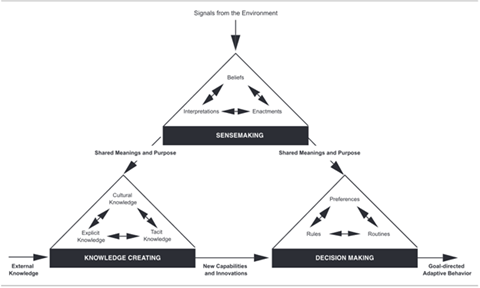
\includegraphics[width=7.16667in,height=\textheight,keepaspectratio]{content/images/Choo.png}
\end{center}

Choo comments that learning organizations will encourage and foster
innovation through this cycle. Innovations and new concepts are created
and evaluated based on the organization's needs and goals. Concepts
created are then tested and re-evaluated before being enacted in other
organizational levels to generate new knowledge creation cycles.

\subsection{Business Process Models}\label{business-process-models}

As we consider ways organizations can learn and know, we can look at
different tools to help sense-making, knowledge creation, and
decision-making. One such tool is the Business Process Model.

Business Process Models (BPMs) are tools that people within the
organization can use to visualize the flow of different processes. These
tools can also help us visualize the organization's and individuals'
information needs at each step of the process. As different individuals
and departments in an organization may come together to complete a task,
so will the information needed to complete that task. By creating
accurate BPMs, organizations can help create transparency for workers,
allowing information needs to be better identified and met.

BPMs will be discussed more in your Information Systems class, but we
can develop a surface understanding of their usefulness in
organizations. Each BPM will have a start point (where the process
begins) and an end point (where the process is complete) and may
describe different steps for each individual involved. The steps for
different individuals may be visually represented in different
``lanes,'' like in the below BPM for a restaurant process. The customer,
host/hostess, waitstaff, chefs, and even the point of sales system are
displayed in their lane. Each lane outlines steps of how and when an
individual will participate in the entire process.

\begin{center}
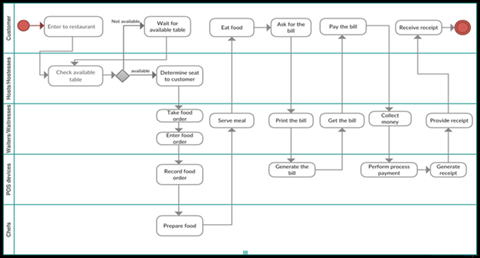
\includegraphics[width=7.03125in,height=\textheight,keepaspectratio]{content/images/BPM.png}
\end{center}

Image source: (Somphanpae and Boonsiri 2016)

By examining each step of the process, we can anticipate what decisions
individuals will have to make during their steps and seek to ensure they
have the information they need. By ensuring that individuals are
equipped with the information they need to complete their steps, we can
help to ensure that the organization can carry out the desired process.

\begin{tcolorbox}[enhanced jigsaw, arc=.35mm, bottomrule=.15mm, bottomtitle=1mm, breakable, colback=white, colbacktitle=quarto-callout-tip-color!10!white, colframe=quarto-callout-tip-color-frame, coltitle=black, left=2mm, leftrule=.75mm, opacityback=0, opacitybacktitle=0.6, rightrule=.15mm, title=\textcolor{quarto-callout-tip-color}{\faLightbulb}\hspace{0.5em}{Pause and Reflect}, titlerule=0mm, toprule=.15mm, toptitle=1mm]

At what point in Choo's model could a BPM be helpful for the
organization -- sense-making, knowledge creation, or decision-making?

\end{tcolorbox}

\section{Embedded Librarianship}\label{embedded-librarianship}

People tend to identify librarians based on the buildings they work in,
thinking that ``a librarian works in a library''. This is not always the
case. As traditional reference services are becoming less common due to
the rise of the internet and the changing role of libraries, librarians
are moving out of physical libraries. Embedded librarianship occurs when
librarians are embedded within organizations and institutions. These
librarians develop strong relationships with the groups of people they
work with, such as faculty, students, a marketing department or a
research team. Embedded librarians are knowledgeable about the work
their team is working on (Shumaker 2012b). ``In order for librarians to
be effective in the learning community, they must be viewed by all as a
partner in the community. Real familiarity with the course and content
is vital to change the perception of students that the librarian is
`just visiting' and is not an integral part of the learning community''
(Muir and Heller-Ross 2010, 92)

Three main factors define embedded librarianship: ongoing relationships,
knowledge of and commitment to shared goals, and customized high-value
contributions (Shumaker 2012b).

\begin{center}
\pandocbounded{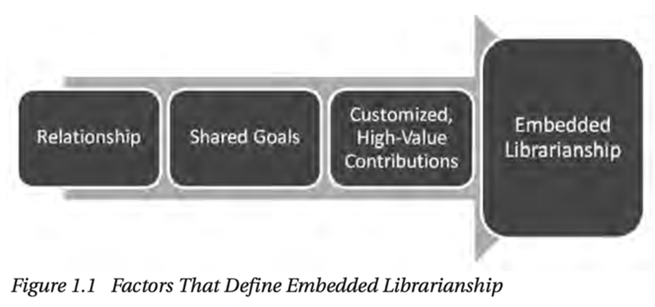
\includegraphics[keepaspectratio]{content/images/Embedded_librarian.png}}
\end{center}

\subsection{Advantages of Embedded
Librarianship}\label{advantages-of-embedded-librarianship}

Embedded librarians can anticipate their patrons' needs; they don't wait
to be asked for help. They work for an entire team and help multiple
people at once. Embedded librarians understand the needs of their team
because they are so familiar with the project. ``With embedded
librarianship, transactions still occur- documents are requested,
instructional sessions are held, or documents are added to a shared
virtual workspace- but the emphasis shifts from the transaction to the
project'' (Shumaker 2012a, 13). Embedded librarianships are responsible
for more than just providing a service.

\subsection{Other Kinds of Mobile
Librarianship}\label{other-kinds-of-mobile-librarianship}

It is not only embedded librarians that move outside of traditional
library spaces. You may find a few different kinds of librarians outside
the library. (Shumaker 2012a)

\begin{itemize}
\item
  \textbf{Virtual librarians}. Virtual librarians are available remotely
  (sometimes 24/7 due to time zones) through phone, email, instant
  messaging or texting. These librarians are similar to traditional
  librarians in that they passively wait to be asked for help.
\item
  \textbf{Roving librarian}. A librarian who sets up in different
  locations such as the classroom or cafeteria. This librarian differs
  from embedded as they are still disconnected from the organization's
  work but are there to answer questions.
\item
  \textbf{Personal librarian}. First-year undergraduate students are
  each assigned their own personal librarian to go to for research help
  throughout their degree. This doesn't work well with how many group
  projects are assigned in universities today, as each student would
  have a different librarian.
\item
  \textbf{Consulting librarian}. Consulting librarians work with either
  a team or an individual client. They establish long-term relationships
  and are always planning for the next project. The only drawback is
  that they aren't always considered part of the team.
\end{itemize}

\section{Case study}\label{case-study-3}

\emph{Wren and Tracey are out for a walk at Point Pleasant on a sunny
Saturday morning in October. Last spring, the gang graduated from the MI
program and have not seen each other since. The two are vecited to catch
up and learn how everything has been going for the last few months.}

\textbf{Wren}: Tracy! It feels like forever since I've seen you; it's so
good to catch up finally!

\textbf{Tracy}: It does feel like it's been ages, but time really does
fly. Hey! Have you heard what Jude and Dante have been up to this
summer?

\textbf{Wren}: Yes- I grabbed dinner with them two weeks ago when they
visited Halifax. Dante got an entry-level position at South Shore Public
Libraries and moved to Lunenburg. Jude has been working as a digital
archivist at a professional organization in Quebec City.

\textbf{Tracy}: That's awesome; they got just the jobs they sought. How
have you been?

\textbf{Wren}: I've been so busy! I was offered a full-time position
with the tech start-up that I did my practicum at starting right after
we graduated, and it's been going well. At my firm, we develop solutions
for businesses to collect and analyze data from their environment to
monitor their performance and inform decisions. Our software has modules
designed for different teams at various levels of the organization. The
Information Management program prepared me for this because I'm part of
the bridge team that works with clients to understand their needs and
the software development team. What about you?

\textbf{Tracy}: I have been doing consultant work. It can be pretty
intense, though; we move from one housefire to another. We primarily
work with small businesses, especially NGOs or non-profits. But their
infrastructure can be\ldots messy. It is good, challenging work. I feel
like I'm contributing to something good at the end of the day, you know?

\textbf{Wren}: It sounds like this job has the potential to be quite
satisfying and fulfilling for you!

\emph{While walking and talking, Wren receives a notification on her
phone. Opening her email, she finds out that a large corporate
organization has bought out the small company she works for.}

\textbf{Wren}: Oh, wow. That was an email from my boss to everyone in
the office. A large organization has just acquired our company! Good
grief!

\textbf{Tracy}: That will be a big change. I dealt with a similar
situation at a job I had in my late twenties. A corporation bought out
the company I was working for, and everyone was apprehensive about how
the transition would go.

\textbf{Wren}: Were people okay with the changes that came about?

\textbf{Tracy}: It was a big challenge at first. It took some time, but
eventually, we ended up better off. I'm still connected with some of my
old coworkers on LinkedIn, and they've told me how happy they are with
how the company culture has developed. In my past work, I've also helped
organizations determine their information needs and implement processes
that address and meet them. But I agree with you -- change is
uncomfortable. Plenty of people at both companies will feel uncertain
about the effects of the change. Do you know this new company?

\textbf{Wren}: I looked at jobs with them when I graduated, but they're
too big for me. I didn't want to go full on corporate -- no offence. I
wanted someplace small where I could learn and see the impact of my
work. Now, being absorbed by a corporate organization\ldots{} I worry
that it may get too bureaucratic and inhibit our efficiency.

\textbf{Tracy}: Yeah, no offence taken -- I get it. And I totally agree
about small businesses -- you learn a lot about how they work. Trust me,
they will want you to be a part of this, especially since you understand
the culture of your workplace. You can help new employees understand
what is essential to your team and make this work. What does
communication look like in your current workplace?

\textbf{Wren}: Since we're a small team, communication essentially
happens in person, by email, and mostly on our shared whiteboard. It's
all a very fast-paced environment with changes happening quickly. No one
is really in charge; it's mostly a collaborative team.

\textbf{Tracy}: Ah, I see. You guys do software\ldots{} so the
environment needs to be quite agile?

\textbf{Wren}: Exactly! We move fast, minimize formal communication, and
basically just get stuff done! Now, we'll have many new external
stakeholders to answer to, potentially delaying our ability to execute
quickly. Our company used to decide on its own internal objectives, and
now we will be tasked with answering to larger-scale goals and external
determinants of value. Before, we were happy to place user-centred
design at the forefront of our company goals and our small successes
were based on integrating customer feedback, but now, at a corporate
level, I'm not sure what benchmarks of success we will have to meet.

\textbf{Tracy}: Yeah\ldots.so change management is going to be critical
here. There are going to be some conflicts in work culture and
communication methods. I hope they have someone that's done this before.

\textbf{Wren}: Well, I know the company quite well; I'm not sure a
larger company seeking to incorporate automated knowledge management
software appreciates the human perspective I bring.

\textbf{Tracy}: I can understand why you might feel this way; it doesn't
feel great to have to constantly defend the importance of your role and
the value you add to the information processes of your organization.

\textbf{Wren}: Yes, exactly, Tracy. In a smaller workplace environment,
it was clear how employees contributed to the work they did and to what
degree. Now, I might be tasked with writing multiple reports a year
outlining how my position is critical to the company's success.

\textbf{Tracy}: I'm sorry, Wren. If it makes you feel better, your
friendship is invaluable to the gang and me. You are a fantastic
communicator, though, so I think as long as you exercise those skills
during this transition period, everything will work out okay. Growing
pains!

Consider the exchange of information and knowledge in the workplaces you
have worked in and the professional environments you have been a part
of. Reflect on the importance of communication and how it impacts the
success of an organization's goals.

\subsection{Discussion Questions}\label{discussion-questions-2}

\begin{itemize}
\item
  What should Wren's company do to ensure a smooth transition with the
  merger? How can they ensure that the information flow stays efficient?
\item
  Consider your current or past places of work- how does information
  flow internally? How does it flow externally?
\item
  Do you find communicating easier in smaller team environments than in
  larger ones? How do communication processes change based on the size
  of the group? How are our environments influenced based on information
  processes?
\item
  Think about how these organizations fit into society in a larger
  context; what role do they play in facilitating communication and
  information flow on a societal level?
\item
  Consider the Data-Information-Knowledge-Wisdom pyramid. Does it seem
  relevant to the organizations you have worked in? How could you
  reimagine it based on the flow of information and knowledge exchange
  in the organizations you have been a part of?
\item
  Do you think there is a difference in how non-profit or
  government-funded organizations share knowledge internally compared
  with for-profit?
\end{itemize}

\section{References}\label{references-5}

\bookmarksetup{startatroot}

\chapter{The Information Economy}\label{the-information-economy}

\section{Learning Objectives}\label{learning-objectives-5}

This chapter aims to get you to consider information as a commodity
(something that can be bought, owned and sold) subject to market forces
and to reflect on the implications for libraries, information
professionals and society at large.

\section{Information in a capitalist
system}\label{information-in-a-capitalist-system}

This section summarizes some of the key elements of Herbert Schiller's
views of the information society, as reported in Webster (2014c).
Schiller's perspective, influenced by his economics background and his
work as a Professor of Communications, played a central role in the
\textbf{political economy} approach to understanding information, which
emphasized the importance of ``looking behind information'' at the
structural features that shape the information produced:

\begin{quote}
\emph{If one wants to understand why newspapers and television produce
particular content, {[}\ldots{]} one ought not to start with an analysis
of journalists, editors, or scriptwriters {[}or of the content
itself{]}. Better far to ask: who owns the operation? What are the
priorities of the business? Where does it make its money?} (Webster
2014c, 152)
\end{quote}

The political economy approach also emphasizes the importance of
considering the capitalist system as a whole, the role of power,
control, and interest, and their significance for the information
society. Some central points of Schiller's theory are market principles
and practices, corporate capitalism, the commodification of information,
and class inequalities.

\subsection{Market principles and
practices}\label{market-principles-and-practices}

According to Schiller, ``the information environment is expressive of
the interests and priorities of corporate capitalism'' (Webster 2014c,
167). The primary purpose of corporations is the generation of profits,
which leads to information being produced and made available only if
profits can be made. This determines what information will be produced,
by whom, for whom, and under what conditions it will be available.
Moreover, under corporate capitalism, these decisions tend to be made by
a limited number of large corporations that form powerful oligopolies.

\subsection{The commodification of
information}\label{the-commodification-of-information}

According to Schiller and others, information is increasingly
commodified to operate in a market society. This means that information
gets to be something one can own, have a price, and be sold or licensed
by a party to another (Webster 2014c). For information to exist as a
commodity, there needs to be a legal framework that supports it, such as
intellectual property law. In Canada, the Copyright Act protects the
rights of content producers by granting them exclusive economic rights
over their work (Al-Sharieh 2018). However, the principle of fair
dealing allows users to use copyrighted information without permission
or payment of royalties. The ``dealing'' must only be for the following
purposes: research, private study, criticism, review, news reporting,
education, satire, or parody. Another exception is when a work is
reproduced in alternative formats to increase accessibility for people
with perceptual disabilities (Al-Sharieh 2018). This highlights the need
for a balance between the rights of the creator and the rights of the
user (such as the right to participate in culture or the right to
education).

Schiller believed that information should be a public good, an idea that
goes entirely against the dominant model. The struggle between the
public good and corporate interests is well illustrated in scholarly
publishing, which we explore in more detail below.

\subsection{Class inequalities}\label{class-inequalities}

Class inequalities also shape how information is produced and
distributed, as class can determine what information one has access to.
This brings us back to the digital divide from Chapter 3 on information
issues. Schiller contends that the information society is one of
``information stratification'' where some (the minority) are
information-rich, and others (the majority, or the ``general public'')
are information-poor. Furthermore, just like unregulated capitalism
naturally leads to monopolies, the natural tendency of this system is to
increase the gap between these two groups.

When the ability to profit determines what information you will have
access to, the information-poor are those who, by having the ability to
pay, end up lumped together in what we call a ``mass market'' to which a
``cheaper'' kind of information can be sold without sacrificing profits.

\begin{tcolorbox}[enhanced jigsaw, arc=.35mm, bottomrule=.15mm, bottomtitle=1mm, breakable, colback=white, colbacktitle=quarto-callout-tip-color!10!white, colframe=quarto-callout-tip-color-frame, coltitle=black, left=2mm, leftrule=.75mm, opacityback=0, opacitybacktitle=0.6, rightrule=.15mm, title=\textcolor{quarto-callout-tip-color}{\faLightbulb}\hspace{0.5em}{Pause and reflect}, titlerule=0mm, toprule=.15mm, toptitle=1mm]

\begin{itemize}
\item
  What may be the effect of the dominance of market principles on the
  information produced, made available, and consumed by the public?
\item
  How do you think we can determine the value of information?
\item
  Do you think that information should be considered a public good? Why?
\item
  Do you think that you are information-poor or information-rich?
\item
  Is there anything that we can do as information professionals to help
  with these issues?
\end{itemize}

\end{tcolorbox}

\section{The case academic publishing
industry}\label{the-case-academic-publishing-industry}

Academic publishing is a highly profitable industry. Here's how it works
in a nutshell. Universities (funded mainly by students and taxpayers)
pay the researchers' salaries. The researchers ask for more public money
to fund their research and hire research assistants, PhDs and postdocs
to do research and write a manuscript to report the research and its
results. They then submit the findings to a journal managed by an
editorial board (all volunteers). One of these volunteers (although
there are exceptions, as some editors-in-chief are paid) will recruit
two or three additional volunteers to evaluate the submitted manuscript.
After two rounds of reviews, the paper will be copy-edited, packaged,
and sold back to the universities who already paid the salaries of all
the people involved in producing and evaluating the work.

Consider the suggested reading below for a much more detailed and
accurate depiction of the industry.

\begin{tcolorbox}[enhanced jigsaw, arc=.35mm, bottomrule=.15mm, bottomtitle=1mm, breakable, colback=white, colbacktitle=quarto-callout-note-color!10!white, colframe=quarto-callout-note-color-frame, coltitle=black, left=2mm, leftrule=.75mm, opacityback=0, opacitybacktitle=0.6, rightrule=.15mm, title=\textcolor{quarto-callout-note-color}{\faInfo}\hspace{0.5em}{Suggested readings}, titlerule=0mm, toprule=.15mm, toptitle=1mm]

The following article is a compelling account of the publishing industry
and its origins.

Buranyi, S. (2017). Is the staggeringly profitable business of
scientific publishing bad for science? \emph{The Guardian}.
\url{https://www.theguardian.com/science/2017/jun/27/profitable-business-scientific-publishing-bad-for-science}

This one is a bibliometric account of how the digital era led to an
increased concentration of the publishing market in the hands of a few
publishers.

Larivière, V., Haustein, S., \& Mongeon, P. (2015). The Oligopoly of
Academic Publishers in the Digital Era. \emph{PLoS ONE}, \emph{10}(6),
e0127502. \url{https://doi.org/10.1371/journal.pone.0127502}

\end{tcolorbox}

In principle, a published research article is unique: ``each journal has
the monopoly on the scientific content of papers it publishes: paper A
published in journal Y is not an alternative to paper B published in
journal Z'' (Larivière et al. 2015). Furthermore, access to published
research is crucial for researchers to stay current with the advances in
their field and compete in a highly competitive research environment.
This allows publishers to increase their prices without influencing
demand, leading to hyperinflation of journal subscription prices that
deplete academic libraries' budgets (Shu et al. 2017).

The digitization of academic publishing and journals created an
opportunity to reduce the cost associated with publishing and storing
scholarly journals. The publishers introduced the journal bundles (the
``Big Deal''), which indeed seemed like good deals until the continuous
price increase of these bundles led libraries back to square one.

\begin{tcolorbox}[enhanced jigsaw, arc=.35mm, bottomrule=.15mm, bottomtitle=1mm, breakable, colback=white, colbacktitle=quarto-callout-note-color!10!white, colframe=quarto-callout-note-color-frame, coltitle=black, left=2mm, leftrule=.75mm, opacityback=0, opacitybacktitle=0.6, rightrule=.15mm, title=\textcolor{quarto-callout-note-color}{\faInfo}\hspace{0.5em}{The cost of access to scholarly journals in Canada}, titlerule=0mm, toprule=.15mm, toptitle=1mm]

The subscription fees paid by Canadian university libraries to some
publishers are reported yearly and are openly available. The latest
release of this data can be found in Brin (2021). Here are the
subscriptions reported for Dalhousie University for the 2019-2020 fiscal
year:

{\def\LTcaptype{none} % do not increment counter
\begin{longtable}[]{@{}
  >{\raggedright\arraybackslash}p{(\linewidth - 2\tabcolsep) * \real{0.7361}}
  >{\raggedleft\arraybackslash}p{(\linewidth - 2\tabcolsep) * \real{0.2639}}@{}}
\toprule\noalign{}
\begin{minipage}[b]{\linewidth}\raggedright
Product
\end{minipage} & \begin{minipage}[b]{\linewidth}\raggedleft
Price (CA)
\end{minipage} \\
\midrule\noalign{}
\endhead
\bottomrule\noalign{}
\endlastfoot
ScienceDirect-Freedom Collection, incl.~Academic Press Collection &
\$1,539,329.53 \\
Wiley Online Library (Database) & \$801,401.41 \\
Taylor \& Francis Journals (SSH/S\&T/Medical) & \$301,280.04 \\
Oxford Journals Online & \$125,574.14 \\
Sage Premier All-Access & \$118,238.42 \\
Web of Science & \$115,703.91 \\
Scopus & \$69,254.69 \\
Cambridge Journals Online & \$62,628.47 \\
Web of Knowledge & \$48,556.76 \\
RSC Electronic Journals & \$23,965.30 \\
NRC Research Press Journals & \$16,348.20 \\
MathSciNet and Consortium Database Fees & \$14,125.01 \\
\textbf{Total} & \textbf{\$3,236,405.88} \\
\end{longtable}
}

\end{tcolorbox}

The unsustainable financial situation has led several universities to
cancel journal subscriptions. In 2016, the Canadian Research Knowledge
Network (CRKN) launched the Journal Usage Project (JUP), a national
evaluation of journal usage in universities to help libraries assess the
state of their collection and either cancel the big deals or negotiate
better prices with publishers. The results of this evaluation shed light
on the concentration of journal use in Canadian universities, with
almost two-thirds of the journals included in the Springer (now
Springer-Nature) being considered essential for none of the universities
included in the study.

\begin{figure}[H]

{\centering 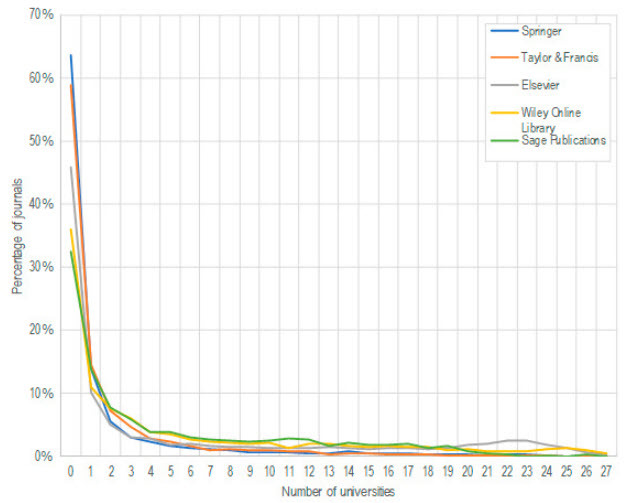
\includegraphics[width=6.9375in,height=\textheight,keepaspectratio]{content/images/core_journals.jpg}

}

\caption{Relative frequency distribution of journals by the number of
universities where they are used significantly (Mongeon et al. 2021).}

\end{figure}%

\begin{tcolorbox}[enhanced jigsaw, arc=.35mm, bottomrule=.15mm, bottomtitle=1mm, breakable, colback=white, colbacktitle=quarto-callout-note-color!10!white, colframe=quarto-callout-note-color-frame, coltitle=black, left=2mm, leftrule=.75mm, opacityback=0, opacitybacktitle=0.6, rightrule=.15mm, title=\textcolor{quarto-callout-note-color}{\faInfo}\hspace{0.5em}{Suggested reading}, titlerule=0mm, toprule=.15mm, toptitle=1mm]

The full results of the analysis sponsored by CRKN's Journal Usage
Project are reported in the following article:

Mongeon, P., Siler, K., Archambault, A., Sugimoto, C., \& Larivière, V.
(2021). Collection Development in the Era of Big Deals. \emph{College \&
Research Libraries}, \emph{82}(2), 219.
\url{https://doi.org/10.5860/crl.82.2.219}

\end{tcolorbox}

\section{Open access}\label{open-access}

Open Access is a movement aiming to make research output freely
available online by removing barriers to access, such as subscription
prices. The Budapest Initiative (BOAI) initially proposed two main
open-access models. The first one, self-archiving (also known as green
open access), allows researchers to deposit their already published
articles in open electronic archives, also known as repositories. The
second one, also known as gold open access, relies on a brand new type
of journal that makes new scientific articles immediately available on
its website, with no copyright restriction. These new journals would not
charge for subscription or access fees. While the original BOAI
declaration suggested that these new journals find alternative sources
of revenue (such as grants or add-ons that could be sold as an extra),
article processing charges (APCs), a publishing fee charged to authors,
emerged as one of the primary sources of funding for OA journals. While
the open access movement may have seemed like a break away from the
commodification of scientific knowledge, the pay-to-publish model turned
out to be, once again, an extremely lucrative business for publishers.
Butler et al. (2022) estimated that the five largest publishers
generated \$1.06 billion in revenues from APCs during 2015-2018.

\begin{tcolorbox}[enhanced jigsaw, arc=.35mm, bottomrule=.15mm, bottomtitle=1mm, breakable, colback=white, colbacktitle=quarto-callout-tip-color!10!white, colframe=quarto-callout-tip-color-frame, coltitle=black, left=2mm, leftrule=.75mm, opacityback=0, opacitybacktitle=0.6, rightrule=.15mm, title=\textcolor{quarto-callout-tip-color}{\faLightbulb}\hspace{0.5em}{Pause and reflect}, titlerule=0mm, toprule=.15mm, toptitle=1mm]

\begin{itemize}
\tightlist
\item
  What role do you academic librarians and other librarians play (or
  could play) in supporting Open Access to the scholarly literature?
\end{itemize}

\end{tcolorbox}

\section{Case study}\label{case-study-4}

\emph{The gang have all moved on from their entry-level jobs and are
starting towards the careers they hoped for while in school. Dante has
become a public librarian at Saskatoon Public Library, Jude is working
at the Nova Scotia Archives, Tracy is a knowledge management corporate
consultant in Montreal's arts and entertainment sector, and Wren has
been promoted at the tech start-up she works for.}

\emph{Dante and Jude attend a library and archives conference in Lake
Como, Italy. The conference party, which takes place on a small, private
boat, features many prominent professionals in Information Management.}

\emph{The air is warm as the two disembark the boat at the end of the
night, discussing the conversations. One speaker that resonated with
both was Mallory Jensen, an Academic librarian from New York State. She
spoke about her work negotiating with publishers to unbundle the
academic journals her library purchases so that libraries can save money
and only buy the journals their library desires.}

\textbf{Jude}: I don't have to deal with the issues surrounding big
academic publishers because I work in archives, but Mallory is
passionate about what she does. She shed light on how this is an issue
with repercussions for all areas of the library. The budget
significantly influences how resources are distributed in library
settings!

\textbf{Dante}: You nailed it, Jude. I have met a few academic
librarians through these types of conferences who are also frustrated by
this issue. It is already so expensive for universities to purchase
these journals. It just seems insane to force them to buy ones they
don't even want.

\textbf{Jude}: It really is! And then, on top of that, it's ludicrous
that universities have to buy back the research they've already paid
their professors to do.

\textbf{Dante}: If only there were a way around it, like if the research
could be found online, students and staff could just download and read
it for free.

\textbf{Jude}: Arrrrghhhh, I know we just got off a boat, but Dante,
you're talking about piracy! Do you think that's a fair solution? How
can you guarantee that the authors are appropriately compensated if
their work is illegally downloaded?

\textbf{Dante}: I guess I never thought about it that way. When there's
a new book I want to read with a long holds list at our library, I
usually just go online and try to find a free copy to download. I figure
I would be reading it for free through the library anyway, so what
difference does it make?

\textbf{Jude}: The difference is that downloading it online is immoral!
That is someone's intellectual property. Waiting for a copy from the
library or purchasing it at a bookshop is the right thing to do. You
could also buy a copy online.

\textbf{Dante}: But why would I buy a digital copy when it's so easily
accessible for free? How can people be successful selling information
online when there's so much available?

\textbf{Jude}: What about open-access journals? There has been a
significant movement towards them. They offer freely accessible content
to democratize knowledge but usually charge publication fees to make the
work they host publicly available. This remedies the problem of the
end-user paying abominable subscription fees, though they carry their
own issues. But at least we are moving in the right direction!

\textbf{Dante}: You're probably right! Speaking of open access, why
don't we just grab an aperitif at that cute little restaurant across the
street? It has a beautiful, uncovered patio, and it's such a warm
evening!

\textbf{Jude}: That's a great idea, oh look! Mallory is sitting with a
couple more conference speakers; let's see if she can offer more
insight!

\subsection{Discussion Questions}\label{discussion-questions-3}

\begin{itemize}
\item
  Do you agree with Dante or Jude? Do you think that it's fair for
  someone to be able to download a PDF of a book for free online when
  others are purchasing it legally? Why?
\item
  What is your opinion on the oligopoly controlling all the academic
  journals libraries purchase?
\item
  Do you think that these journal bundles should be unbundled? Why?
\item
  How do we determine value differently on an individual versus
  collective basis?
\item
  Are you able to find your institution's policy on Open-Access? How can
  institutional repositories and libraries help facilitate open-access
  publishing among faculty and students?
\item
  Find 1-2 open-access journals online and try to determine how they
  generate revenue. What are your thoughts on the open-access movement?
\end{itemize}

\section{References}\label{references-6}

\bookmarksetup{startatroot}

\chapter{The Attention Economy}\label{the-attention-economy}

\section{Learning objective}\label{learning-objective-1}

This week's discussion is around the concept of the attention economy,
which is fundamentally distinct from the information economy (but not
entirely separated from it) because it is an economy where information
tends to be free.

\begin{tcolorbox}[enhanced jigsaw, arc=.35mm, bottomrule=.15mm, bottomtitle=1mm, breakable, colback=white, colbacktitle=quarto-callout-tip-color!10!white, colframe=quarto-callout-tip-color-frame, coltitle=black, left=2mm, leftrule=.75mm, opacityback=0, opacitybacktitle=0.6, rightrule=.15mm, title=\textcolor{quarto-callout-tip-color}{\faLightbulb}\hspace{0.5em}{Pause and reflect}, titlerule=0mm, toprule=.15mm, toptitle=1mm]

If information is free, then what are the commodities that are produced,
owned and sold in this new market?

\end{tcolorbox}

We will also explore one of the corollaries of this new economy, which
is a heightened capacity for the surveillance of individuals and the
resulting threat to privacy.

\section{From information scarcity to attention
scarcity}\label{from-information-scarcity-to-attention-scarcity}

If we think about a market system, what is within this system that
contains value? That which is valuable to consumers. And, how is the
value of something calculated? By demand. A product which is in high
demand is generally more difficult to keep ``on the shelves'' or
in-stock. If a product is highly sought-after, it becomes purchased; if
purchased often enough, the product becomes scarce; if something becomes
scarce (or rare), the purchasing cost is likely to go up. Rare items
within a market system are expensive; commonly found items, or items in
overabundance, are cheaper.~~

How does this relate to an information economy? Certainly, information
is not scarce in this context. As Simon (1971) states:

\begin{quote}
``{[}I{]}n an information-rich world, the wealth of information means a
dearth of something else: a scarcity of whatever it is that information
consumes. What information consumes is rather obvious: it consumes the
attention of its recipients. Hence a wealth of information creates a
poverty of attention and a need to allocate that attention efficiently
among the overabundance of information sources that might consume it.''
\end{quote}

In an information economy, in which we are an informatic personhood
(Lee, 2021), our attention is the means by which we ``pay'' for
information services. Our attention is paid through our time and energy
spent investing in an information economy. For example, scrolling
through TikTok videos for hours is a way you ``spend'' your attention in
this economical context. Your attention is the rare, scarce item within
the information economy; there is a limited amount of it to go around
(i.e., split between work, sleeping, eating, showering, etc.). Due to
this fact, competitors within the information economy will try different
tactics to grab hold of your attention. Notifications or pop-ups are
ways in which a competitor tries to ``bid'' for your attention. As soon
as you divert away from one information context, such as TikTok, to
another, such as Instagram, that information economy has successfully
``purchased'' your attention. Different social media platforms have
invested in various ways to hold onto your attention once they have
initially grabbed it; for example, Facebook now automatically plays
videos on your News Feed, instead of you having to push ``play'' each
time.~~

Watch the following video, ``The Attention Economy: How They Addict
Us,'' here:

\begin{tcolorbox}[enhanced jigsaw, arc=.35mm, bottomrule=.15mm, bottomtitle=1mm, breakable, colback=white, colbacktitle=quarto-callout-tip-color!10!white, colframe=quarto-callout-tip-color-frame, coltitle=black, left=2mm, leftrule=.75mm, opacityback=0, opacitybacktitle=0.6, rightrule=.15mm, title=\textcolor{quarto-callout-tip-color}{\faLightbulb}\hspace{0.5em}{Pause and reflect}, titlerule=0mm, toprule=.15mm, toptitle=1mm]

Do you think there is a way to ``escape'' the attention economy? Do you
think, between the choices of opting out of the system entirely or
figuring out how to reshape the current system, one is more realistic or
desirable than the other? Why or why not?

\end{tcolorbox}

\section{Information wants to be
free}\label{information-wants-to-be-free}

When \href{https://www.britannica.com/}{Encyclopedia Britannica} went
online, its publisher decided to offer its content for free. ``It's the
new business paradigm,'' says an executive at the company, ``information
wants to be free'':~

\begin{quote}
``Basically we are a content company and we believe we should deliver in
whatever form users need it. We made it free because we felt it was the
only way to get the critical mass of people visiting the site that we
need to make money from sponsorship and e-commerce.'' (Fischer 2008)
\end{quote}

When a user consumes information for free, the way in which a company
makes money is from advertisements. However, users often do not enjoy
being bombarded with advertisements when browsing an information
resource. Advertisements may even deflect or deter a user from
continuing to invest/spend their attention resources within a certain
context. This may lead users to ``purchase'' the ``free'' (I.e., paying
for a premium YouTube account with no advertisements, versus using
YouTube for free with advertisements). What strategies can be used by
companies to ``sell'' what is otherwise freely available?

\section{How to ``sell'' the free}\label{how-to-sell-the-free}

According to Kelly (2008), there are several strategies that we or a
company can employ to ``sell'' free information in an attention
economy:~~

\begin{itemize}
\item
  \textbf{Immediacy} -- getting the information you want, when you want
  it; having no need to wait around to access the freely available
  information (I.e., paying a bit extra to see a movie in theatres
  versus waiting for it to be freely accessible on a streaming media
  provider, like Kanopy or Hoopla provided by Halifax Public Libraries).
  ~
\item
  \textbf{Personalization} -- a personalized copy of an information
  resource, which motivates the user to pay for what would otherwise be
  free.
\item
  \textbf{Interpretation} -- providing a paid service (like technical
  assistance) for free software or instructional information (I.e.,
  technical support provided by TELUS will charge you money to speak to
  a representative over the phone, whereas the same information online
  can be found for free).~
\item
  \textbf{Authenticity} -- paying for the ``authentic'' version of a
  software/information that is ``tried and true'' (I.e., paying for the
  authentic version of a Taylor Swift recording via a Spotify
  subscription versus downloading the song freely {[}illegally{]} at a
  potentially lower quality).
\item
  \textbf{Accessibility} -- paying for backups and storage of online
  information (i.e., iCloud).
\end{itemize}

\begin{itemize}
\item
  \textbf{Embodiment} -- paying for the experience of being in an
  information setting with other ``users'' (I.e., paying to see multiple
  bands perform at a music festival versus watching a recording of those
  performances online) ~
\item
  \textbf{Patronage} -- paying a fee to support your favourite
  authors/artists/creators; those within a ``fandom'' will opt to
  support the creation of their favourite works, so long as it is easy
  to do so.
\item
  \textbf{Findability} -- information that is free may sometimes be more
  difficult and time-consuming to find.
\end{itemize}

\begin{tcolorbox}[enhanced jigsaw, arc=.35mm, bottomrule=.15mm, bottomtitle=1mm, breakable, colback=white, colbacktitle=quarto-callout-tip-color!10!white, colframe=quarto-callout-tip-color-frame, coltitle=black, left=2mm, leftrule=.75mm, opacityback=0, opacitybacktitle=0.6, rightrule=.15mm, title=\textcolor{quarto-callout-tip-color}{\faLightbulb}\hspace{0.5em}{Pause and reflect}, titlerule=0mm, toprule=.15mm, toptitle=1mm]

What strategies are/could be used by libraries to ``sell'' the free?

\end{tcolorbox}

\section{Selling attention or selling
data}\label{selling-attention-or-selling-data}

\begin{quote}
``Today, information II {[}information generated by users of the Web
2.0{]} is completely commodified, it is virtually inaccessible to anyone
except new media companies, who have the legal and technological means
to render massive quantities of information II into commodities.''
(Fischer 2008)
\end{quote}

``Information II'' is transactional information: the information about
the transactions that we make and our other activities on the web, which
informs third parties about our socio-demographic characteristics and
the details of our everyday lives, as opposed to ``Information I'' that
we consume and informs us. In an attention economy, when everything is
free, you are the product. By choosing to spend or allocate our
attention to one resource over another, this is how we volunteer to be
and exist within an attention economy platform. The ways in which we
browse, search, stream, or select media become data that is generated
about us, commodified, and sold. Companies use strategies for
attention-grabbing, such as some of those we discussed in Section 8.4.
Advertisers watch online habits to better provide more streamlined
advertisements to best suit your attention-driven needs.

Watch the following TEDTalk by Tristan Harris on ``How a handful of tech
companies control billions of minds every day'' here:

\section{Privacy and consent}\label{privacy-and-consent}

Organizations need our consent to collect data about us. How do they get
us to consent? Through strategies of digital resignation (Draper and
Turow 2019). Digital resignation refers to the phenomenon in which
individuals feel that attempts to control the amount and type of
information collected about them digitally are futile. There is a
discrepancy between people's attitudes and behavior around privacy,
namely, people say that privacy is important to them, but act in a way
that is contrary to that belief (Kokolakis 2017). This sense of futility
has been cultivated, specifically in corporate spaces, to make
individuals see ``corporate power as an inevitable and immovable feature
of contemporary life.'' (Draper and Turow 2019)~

\begin{center}
\pandocbounded{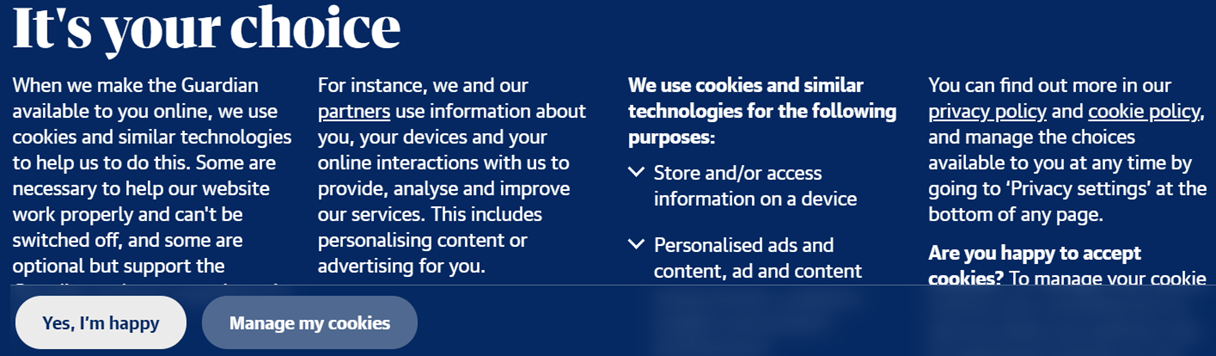
\includegraphics[keepaspectratio]{content/images/paste-46565D69.png}}
\end{center}

Above is an example of a company employing digital resignation. While
the language suggests that this is an opportunity for the reader to make
their own choice, the amount of text, language, and design contribute to
making this overly complicated, prompting users to just click through
quickly to get past the jargon.~

\begin{tcolorbox}[enhanced jigsaw, arc=.35mm, bottomrule=.15mm, bottomtitle=1mm, breakable, colback=white, colbacktitle=quarto-callout-tip-color!10!white, colframe=quarto-callout-tip-color-frame, coltitle=black, left=2mm, leftrule=.75mm, opacityback=0, opacitybacktitle=0.6, rightrule=.15mm, title=\textcolor{quarto-callout-tip-color}{\faLightbulb}\hspace{0.5em}{Pause and reflect}, titlerule=0mm, toprule=.15mm, toptitle=1mm]

What choices are being made in the above image that could result in
digital resignation? How would you design an alternative to support
authentic consent?~

Even though you are providing small amounts of information across
different platforms, computers will generate extremely precise data
about you by bringing the data all together. Computers can amplify but
also distort our data\ldots{} can we trust in these processes?~

\end{tcolorbox}

\section{Trust in the machine?}\label{trust-in-the-machine}

Over time, platforms can collect thousands of data points for a single
user and compile this information into a kind of profile that can be
used in recommendation algorithms that push content to users. The goal
of platforms is to get users to remain online, viewing content (and ads)
for as long as possible. Therefore, the recommendation algorithms are
key in accurately predicting what a person might like to see, and
therefore, keeping them engaged on the platform. TikTok, which is
increasingly popular, specifically with young people, has employed an
unprecedented centring of algorithmically driven feeds in the For You
page (Bhandari and Bimo 2022).

While these algorithms do succeed in predicting the content a user would
like to see, and keep them engaged on the platform, this can lead to
untruthful and unreliable content being boosted, if the algorithm
predicts that it has a large enough audience. AI has been shown to
display a lack of fairness, and reinforce stereotypes of specific
gender, racial, and cultural groups (Panch et al. 2019). In the United
States, politicians have identified social media algorithms as a major
contributor to the spread of misinformation that culminated in the
January 6th insurrection (Morrison 2021).

Watch the following Crash Course video on ``Algorithmic Bias and
Fairness'' here:~

\begin{tcolorbox}[enhanced jigsaw, arc=.35mm, bottomrule=.15mm, bottomtitle=1mm, breakable, colback=white, colbacktitle=quarto-callout-tip-color!10!white, colframe=quarto-callout-tip-color-frame, coltitle=black, left=2mm, leftrule=.75mm, opacityback=0, opacitybacktitle=0.6, rightrule=.15mm, title=\textcolor{quarto-callout-tip-color}{\faLightbulb}\hspace{0.5em}{Pause and reflect}, titlerule=0mm, toprule=.15mm, toptitle=1mm]

In what ways do you think it's good to collect large amounts of
information about people?~~~

\end{tcolorbox}

\section{Surveillance and
organization}\label{surveillance-and-organization}

Routine surveillance is required for effective organization:~

\begin{quote}
``To organize life information must be systematically gathered on people
and their activities. We must know about people if we are to arrange
social life: what they buy, and when and where; how much energy they
require, where and at what times; how many people there are in a given
area, of what gender, age and state of health; what tastes, lifestyles
and spending capacities given sectors of the populations enjoy.''
(Webster 2014d)
\end{quote}

Government organizations, like Statistics Canada collect data that can
help decision makers in evidence-based practice. Companies also collect
data to improve customer experiences and address negative experiences.
Without data collection, we would be unable to make decisions based on
empirical information and would only be relying on opinions and
preferences. All this is to say, data collection results in enhancements
in our daily life, productivity and happiness. We can make more informed
decisions if we have access to data.

\section{Heightened reflexivity}\label{heightened-reflexivity}

\begin{quote}
``Modernity being a matter of increased choices made at every level
necessitates \textbf{heightened reflexivity}, {[}which requires{]}
\textbf{increased surveillance} so that we may develop knowledge upon
which may be made choices about \textbf{ourselves} and the sort of
\textbf{society} we want.'' (Webster 2014d)
\end{quote}

In addition to the larger decisions discussed in Section 8.8, data can
support us in reflexive thought. An athlete looking to improve their
marathon time could rely on data from their smartwatch to gain an
understanding of their fitness and their training. A library director
could review circulation numbers to help them determine what
books/movies/resources their patrons enjoy the most, and what they
should aim to buy more of, and weed in the future. This data can help us
add value to our own lives, and the organizations we work for.~~

\begin{tcolorbox}[enhanced jigsaw, arc=.35mm, bottomrule=.15mm, bottomtitle=1mm, breakable, colback=white, colbacktitle=quarto-callout-tip-color!10!white, colframe=quarto-callout-tip-color-frame, coltitle=black, left=2mm, leftrule=.75mm, opacityback=0, opacitybacktitle=0.6, rightrule=.15mm, title=\textcolor{quarto-callout-tip-color}{\faLightbulb}\hspace{0.5em}{Pause and reflect}, titlerule=0mm, toprule=.15mm, toptitle=1mm]

What data do you intentionally collect and analyze (screentime, step
count, etc.)? Do you feel this helps bring you closer to your personal
goals?~

\end{tcolorbox}

\section{Case study}\label{case-study-5}

\emph{An outbreak has sent countries across the globe into lockdown.
Jude works at the Nova Scotia Archives, and they have directed their
employees to work from home in accordance with provincial regulations.
Jude initially finds a stable routine helpful; he wakes up in the
morning, takes his dog Kevin on a walk, and then begins his workday. As
the months go by, Jude finds himself consuming more and more online
content instead of doing the things he regularly enjoys. Jude begins to
immerse himself heavily in the perspectives of certain online forums and
media. The gang grows concerned with Jude's online behaviours and
collectively check in with him in their group chat.}

\textbf{Info Masters: Group Chat}

\emph{3:07am}

\textbf{In\_perpe\_jude\_ity87}: Hey friends, check out this YouTube
video when you get a chance- really interesting perspective\ldots{} not
something you'll hear on the mainstream media.

\emph{9:45am}

\textbf{Trace\_2\_face\_consultation}: Good morning Jude, et al.~I see
you were up really late Jude, were you just watching videos all night?

\textbf{Dantes\_infern0}: Rise and shine team! Let's manage information
😊

\textbf{tWrending\_in\_tech}: Good morn!! Hmm\ldots{} I saw this the
other day when it was floating around the internet\ldots{} but only
cause I've got to keep my finger on the pulse of the web and not because
it's content I usually watch\ldots{} where did you find this, Jude?

\textbf{In\_perpe\_jude\_ity87}: Haha, yeah, I was up pretty late. I
just kinda fell down a rabbit hole in this online forum I'm a part of
and next thing I knew it was 3am. Gotta stop doing that! Let me know
what you think about the video.

\textbf{Trace\_2\_face\_consultation}: Oh dear- Jude, it sounds like
nights like that have become the norm? That doesn't seem like a very
healthy lifestyle. Why are you up so late every night?

\textbf{Dantes\_infern0}: From the activity logs I can view on the
social sites we're all a part of you seem pretty active on a few
different pages and groups. Take a break, my Jude!

\textbf{In\_perpe\_jude\_ity87}: I don't need a break. I'm just really
curious and interested in learning about viewpoints I've never been
exposed to. I've been finding so much new information from videos and
articles shared in these groups.

\textbf{tWrending\_in\_tech}: Awe, Jude- we've always loved your love of
analog formats! So, this comes as a bit of a surprise. It seems like
your attention has been captivated by these groups- just based on what I
see you reposting and chatting about! (Please don't be mad, just
checking in- ily)

\textbf{Trace\_2\_face\_consultation}: Well said, Wren! I remember when
I first got a few online platforms- I couldn't tear myself away! There
was always new and exciting information out there and everything always
felt so urgent. I was afraid to log off and miss new content.

\textbf{Dantes\_infern0}: Hahaha- when I first got Facebook, I remember
joining so many groups dedicated to raising tropical fish. I got REALLY
into it, but after a while, I realized the algorithm was designed to
show me things I liked and interacted with. It kind of becomes a
positive feedback loop. I'm still leaving fish groups, and that was 5
years ago. I also purchased a fair few fish tanks- dang targeted ads!

\textbf{tWrending\_in\_tech}: Hilarious, because I've never seen you
keep a plant alive for more than a week. Dante's inferno indeed. Jude,
as someone who works in tech, could I kindly suggest that you be careful
about where you are investing your attention and time? Some online sites
and apps are designed to capture and monetize your attention and aren't
necessarily concerned with the well-being of users\ldots{} they're more
interested in generating traffic on their sites.

\textbf{In\_perpe\_jude\_ity87}: No one is forcing me to be active on
these groups though\ldots{} the algorithm is working because I'm
genuinely interested in this stuff. It's free, too! The users are the
ones creating all the content. I appreciate your concern, but I think I
just get really into stuff, like the time I got back into baking
sourdough bread at the start of the outbreak LOL.

\textbf{Trace\_2\_face\_consultation}: Thanks for that perspective,
Wren! It is so easy to feel like we are in control because we are the
ones clicking, but many online business models are designed to keep us
on their sites. Our attention is a resource and should be protected and
treated as such! Remember our Professor in Info in Society in first year
telling us ``If it's free, you are the product''? It seems like the
information you are finding is a valuable asset here but in reality, the
data we provide is more valuable to these companies than the information
we obtain from them\ldots{} at least monetarily. And I understand that,
Jude. You are someone who is wholeheartedly invested in what you care
about, and that is such a wonderful characteristic of yours! But often
our strengths and weaknesses go hand in hand- there is no harm in baking
bread, but the viewpoints and content you are consuming so much of can
potentially be a bit dangerous, in insidious ways.

\textbf{Dantes\_infern0}: I saw a documentary about this recently! These
sites are gathering and selling our data. They want users on their sites
as long as possible to offer up more of their personal information. They
track user behaviours so that they have more generated data to sell.
It's a cycle. Some people get in the habit of consuming information
non-stop and don't realize what they are offering in exchange for it.

\textbf{tWrending\_in\_tech}: Agreed! That's why I cap my screen time
now and only go on my social sites intentionally and with premeditated
purpose. Otherwise, I just scroll endlessly!

\textbf{In\_perpe\_jude\_ity87}: I'm surprised by your reactions. I just
shared a video I thought was interesting and didn't mean to cause an
entire discourse on the commodification of our attention\ldots{} talk
about diverting attention away from the main point.

\textbf{tWrending\_in\_tech}: We just want to make sure you are okay,
Jude! With so much information and online content being created
non-stop, the only limiting factor is really our attention. I have
learned to be more mindful since working in tech. As someone with the
inside scoop when it comes to algorithms, they have the potential to
create and reinforce stereotypes, biases, and oppression. It's our
social responsibility to be cognizant of that fact and question what we
are consuming and why. That's just one techie's opinion!

\textbf{In\_perpe\_jude\_ity87}: Well, thanks for your concern, folks.
I'll take your advice and log off- I've got to get back to work. The
fonds won't fawn over themselves, haha. Ttyl!

\textbf{Trace\_2\_face\_consultation}: Thanks for the morning chat, all!
Glad we got to check in with you, Jude!

\textbf{Dantes\_infern0}: Yeah- this convo has made me consider public
libraries' roles in protecting patrons' privacy and not revealing what
resources are used and by whom. I'm going to go see what books we carry
on these topics.

\textbf{tWrending\_in\_tech}: And I'll get back to my big evil tech
company! Bahaha \textgreater:) jk. Have a lovely day all!

\emph{Chat ended.}

Consider the themes discussed in the group chat. The gang observes that
Jude's attention has been monopolized by online groups sharing distinct
points of view. They raise concerns over Jude's level of awareness
regarding the commodification of user attention and urge him to be
mindful of this fact as he navigates online landscapes.

\section{Discussion Questions}\label{discussion-questions-4}

\begin{itemize}
\item
  Would you consider Jude's online behaviours healthy?
\item
  Consider how Jude exists as a user in online settings: do you think he
  feels/is in control? Do you feel as though he possesses a level of
  awareness regarding the time he is spending online and the ways in
  which he is interacting with content?
\item
  Do you feel as though you have a level of agency over the information
  you provide online? When you offer up your data to online sites, does
  it transform from personal information into a commodity? How do you
  perceive personal versus collective versus organizational ownership of
  data online? Is this based on how it was created/generated, or by
  whom?
\item
  Is our data inherently of value? How is value added to the data we
  generate digitally?
\item
  To what degree are you informed about the ways online sites use your
  information? Is it important to you to be aware of how your attention
  is captured and commodified? In what ways can we facilitate greater
  awareness surrounding the attention economy in ourselves and in
  others?
\item
  How do we ensure equitable access to information in an ethical way?
\item
  What are the implications of the attention economy for information
  access, quantity, quality, and behaviour?
\item
  How do the phenomena discussed in this chapter apply to individuals or
  collectives that are not necessarily or directly generating revenues
  out of the attention and information about others?
\end{itemize}

\section{References}\label{references-7}

\bookmarksetup{startatroot}

\chapter{Misinformation, Disinformation, and Fake
News}\label{misinformation-disinformation-and-fake-news}

\section{Learning Objectives}\label{learning-objectives-6}

Earlier in the semester, we spoke about information quality and how the
information we consume can shape our worldviews. In this chapter, we
will return to this issue and dive deeper into the definitions of
misinformation, disinformation and fake news. We will consider the
origins of misinformation, how it spreads, and societal costs. Lastly,
we will discuss how to reduce the impact of misinformation and what we,
as information professionals, can do.

\section{Definitions}\label{definitions}

The main difference between misinformation and disinformation is the
intent behind it. Misinformation occurs when someone unknowingly shares
false information under the pretense that it is true, whereas
disinformation occurs when someone deliberately creates and shares
information they know is false (De Paor and Heravi 2020). Fake news has
been defined in many different ways but generally can be seen as false
news articles that mislead the reader (De Paor and Heravi 2020). Fake
news is co-constructed by its audience because it automatically becomes
fiction if the audience does not believe it. There are many kinds of
fake news, including satire, parody, fabrication, advertising and
propaganda. The major problem is that fake news creators are making
money off this societal trend and are, therefore, motivated to make
believable false news stories (De Paor and Heravi 2020).

\begin{tcolorbox}[enhanced jigsaw, arc=.35mm, bottomrule=.15mm, bottomtitle=1mm, breakable, colback=white, colbacktitle=quarto-callout-tip-color!10!white, colframe=quarto-callout-tip-color-frame, coltitle=black, left=2mm, leftrule=.75mm, opacityback=0, opacitybacktitle=0.6, rightrule=.15mm, title=\textcolor{quarto-callout-tip-color}{\faLightbulb}\hspace{0.5em}{Pause and Reflect}, titlerule=0mm, toprule=.15mm, toptitle=1mm]

\begin{itemize}
\tightlist
\item
  Can you think of a time when you have knowingly or unknowingly spread
  false information?
\item
  Have you ever encountered fake news?

  \begin{itemize}
  \tightlist
  \item
    Did you believe that it was true?
  \item
    Did it in any way shape your actions?
  \end{itemize}
\item
  Can you think of an example of news satire?

  \begin{itemize}
  \tightlist
  \item
    What do you think the intentions behind it are?
  \item
    What is a well-known news parody website?
  \item
    Have you ever believed an article shared through one of these sites?
  \end{itemize}
\end{itemize}

\end{tcolorbox}

\section{Origins of Misinformation}\label{origins-of-misinformation}

Misinformation can arise in many different ways. One way is that rumours
and fiction may be considered to be true. People are more likely to pass
on information that evokes emotion regardless of if it is truthful. This
is a common occurrence with information gleaned through gossip. People
may also read fictional stories and believe their reading is accurate
(Lewandowsky et al. 2012).

The government and politicians are also known to spread misinformation.
People often cannot determine which information is true or false,
especially surrounding elections. People often expect to encounter some
misinformation during elections (Lewandowsky et al. 2012).

The media, including social media, are also spreaders of misinformation.
The media can take accurate information from scientific studies and
twist it in a way that can be misinterpreted- by oversimplifying,
misrepresenting or over-dramatizing scientific results. The media often
tries to portray balanced stories, but sometimes, this can create
misleading outcomes. Social media, too, is a vast spreader of
misinformation. Anyone can post information online without professional
editors or fact checkers verifying the truthfulness of their statements.
Hoax websites exist solely to spread misinformation- and disinformation.
Selective exposure may also occur if people only seek out media sources
that confirm their beliefs (Lewandowsky et al. 2012).

\begin{tcolorbox}[enhanced jigsaw, arc=.35mm, bottomrule=.15mm, bottomtitle=1mm, breakable, colback=white, colbacktitle=quarto-callout-tip-color!10!white, colframe=quarto-callout-tip-color-frame, coltitle=black, left=2mm, leftrule=.75mm, opacityback=0, opacitybacktitle=0.6, rightrule=.15mm, title=\textcolor{quarto-callout-tip-color}{\faLightbulb}\hspace{0.5em}{Pause and Reflect}, titlerule=0mm, toprule=.15mm, toptitle=1mm]

\begin{itemize}
\item
  What is an example of a fictional story that was believed to be true?
\item
  Can you think of a time when the media may have presented you with
  misleading information?
\end{itemize}

\end{tcolorbox}

\section{How does misinformation
spread?}\label{how-does-misinformation-spread}

The internet creates filter bubbles in which people's social media feeds
and Google searches are filtered only to include information that aligns
with their current beliefs. In the Ted Talk below, Eli Pariser describes
filter bubbles as ``your own personal, unique universe of information
you live in online''. The main problem with this is that people are not
shown any opposing views, which only strengthens their current views. If
the views held are false, they will still be shown more information that
aligns with them.

People believe and spread misinformation for a myriad of reasons. People
often don't know that something is misinformation until it is corrected.
Even then, they may have difficulty believing the corrected information
if it does not align with their beliefs. Worldview and personal ideology
play a role in people's willingness to believe misinformation- people
will often argue anything that goes against their pre-existing worldview
(Lewandowsky et al. 2012). People also struggle to identify whether or
not a source is reliable. If an information source is persuasive, people
are more likely to believe it is credible. People so rarely look into
their sources that most often, people remember the gist of the
information they read but not the source it came from. This shows how
important it is for people to consider the sources they are getting
their information from and whether they may be biased or misleading. It
has also been shown that retractions often don't work -- people
sometimes believe the information more after a retraction because they
have been repeatedly exposed to it. This is because the more familiar
information becomes, the truer it can seem (Lewandowsky et al. 2012).

\begin{tcolorbox}[enhanced jigsaw, arc=.35mm, bottomrule=.15mm, bottomtitle=1mm, breakable, colback=white, colbacktitle=quarto-callout-tip-color!10!white, colframe=quarto-callout-tip-color-frame, coltitle=black, left=2mm, leftrule=.75mm, opacityback=0, opacitybacktitle=0.6, rightrule=.15mm, title=\textcolor{quarto-callout-tip-color}{\faLightbulb}\hspace{0.5em}{Pause and Reflect}, titlerule=0mm, toprule=.15mm, toptitle=1mm]

With a friend, Google something related to a current event happening in
the world and compare your results. For example, ``Covid-19'' or
``Martha's Vineyard''. See if you receive the same results.

\begin{itemize}
\item
  Were you surprised by the outcome?
\item
  How do you check that the sources you are reading are credible?
\item
  Is it something you think that you could improve on?
\item
  How would you teach others to do the same?
\end{itemize}

\end{tcolorbox}

\section{Societal costs}\label{societal-costs}

There are many societal costs of misinformation and disinformation. One
major one is that if a large majority believe in misinformation, then
that misinformation can shape political decisions. This would not be in
the best interest of society.

\begin{tcolorbox}[enhanced jigsaw, arc=.35mm, bottomrule=.15mm, bottomtitle=1mm, breakable, colback=white, colbacktitle=quarto-callout-tip-color!10!white, colframe=quarto-callout-tip-color-frame, coltitle=black, left=2mm, leftrule=.75mm, opacityback=0, opacitybacktitle=0.6, rightrule=.15mm, title=\textcolor{quarto-callout-tip-color}{\faLightbulb}\hspace{0.5em}{Pause and Reflect}, titlerule=0mm, toprule=.15mm, toptitle=1mm]

Can you think of any other societal costs of misinformation or
disinformation?

\end{tcolorbox}

\section{Reducing the impact of
misinformation}\label{reducing-the-impact-of-misinformation}

There are many ways to combat misinformation and help people make more
informed decisions about what they read and believe. One way to do this
is to warn people that it may be untrue when they receive information.
It is more helpful if the warning is given before the false information.
If a retraction is necessary, it must be repeated to make the accurate
information more memorable. Another good way to combat misinformation is
to provide an alternative plausible explanation explaining why the
misinformation was considered initially accurate. Lastly, promoting
healthy skepticism can help reduce people's susceptibility to
misinformation by making them question the information they are given
(Lewandowsky et al. 2012).

\begin{tcolorbox}[enhanced jigsaw, arc=.35mm, bottomrule=.15mm, bottomtitle=1mm, breakable, colback=white, colbacktitle=quarto-callout-tip-color!10!white, colframe=quarto-callout-tip-color-frame, coltitle=black, left=2mm, leftrule=.75mm, opacityback=0, opacitybacktitle=0.6, rightrule=.15mm, title=\textcolor{quarto-callout-tip-color}{\faLightbulb}\hspace{0.5em}{Pause and Reflect}, titlerule=0mm, toprule=.15mm, toptitle=1mm]

\begin{itemize}
\item
  What do you think is an excellent way to promote healthy skepticism?
\item
  If you had a friend who believed in misinformation, how would you go
  about helping them to see that it is false?
\end{itemize}

\end{tcolorbox}

\section{What can information professionals
do?}\label{what-can-information-professionals-do}

Librarians can be seen working on the front lines of the battle against
misinformation. In the past, librarians acted as fact-checkers, but in
the future, they must act as educators. This is because librarians
cannot keep up with the level of online misinformation. One way to do
this is to hold information literacy classes at the library. Information
literacy has been cited as an effective way to deal with misinformation
and fake news. It has been defined as ``the ability to think critically
and make balanced judgements about any information we find and use'' (De
Paor and Heravi 2020, 4). Information literacy is an empowerment tool
because it gives people the skills to make informed decisions and
participate fully in society. Other ways that librarians can help combat
fake news is through fact-checking websites, and creating LibGuides.

\begin{tcolorbox}[enhanced jigsaw, arc=.35mm, bottomrule=.15mm, bottomtitle=1mm, breakable, colback=white, colbacktitle=quarto-callout-tip-color!10!white, colframe=quarto-callout-tip-color-frame, coltitle=black, left=2mm, leftrule=.75mm, opacityback=0, opacitybacktitle=0.6, rightrule=.15mm, title=\textcolor{quarto-callout-tip-color}{\faLightbulb}\hspace{0.5em}{Pause and Reflect}, titlerule=0mm, toprule=.15mm, toptitle=1mm]

In what ways do you think that information professionals are responsible
for combating misinformation? How do you see misinformation,
disinformation or fake news impacting you in your future career?

\end{tcolorbox}

\begin{tcolorbox}[enhanced jigsaw, arc=.35mm, bottomrule=.15mm, bottomtitle=1mm, breakable, colback=white, colbacktitle=quarto-callout-note-color!10!white, colframe=quarto-callout-note-color-frame, coltitle=black, left=2mm, leftrule=.75mm, opacityback=0, opacitybacktitle=0.6, rightrule=.15mm, title=\textcolor{quarto-callout-note-color}{\faInfo}\hspace{0.5em}{Suggested Reading}, titlerule=0mm, toprule=.15mm, toptitle=1mm]

If you want to learn more about the different kinds of fake news and how
librarians can help combat it, look at this article.

De Paor, S., \& Heravi, B. (2020). Information literacy and fake news:
How the field of librarianship can help combat the epidemic of fake
news. The Journal of Academic Librarianship, 46(5), 102218.
\url{https://doi.org/10.1016/j.acalib.2020.102218}

If you are interested in the psychological side of why people believe in
misinformation, read this article:

Lewandowsky, S., Ecker, U. K. H., Seifert, C. M., Schwarz, N., \& Cook,
J. (2012). Misinformation and Its Correction: Continued Influence and
Successful Debiasing. Psychological Science in the Public Interest,
13(3), 106--131. \url{https://doi.org/10.1177/1529100612451018}

\end{tcolorbox}

\section{Case Study}\label{case-study-6}

\emph{Jude, always the activist and helpful community member, offers
help to another member of an online forum who has been trying to start a
podcast. Jude has had extensive experience creating and distributing
podcasts as part of working with the LGBTQ Archives and helped community
members create their podcast platforms. After getting the infrastructure
set up and hearing from the forum member that the podcasts were doing
well, a month later, Jude finally had time to listen in on the latest
episode. Alarmed, Jude calls Dante late at night.}

*The phone rings, waking Dante up*

\textbf{Dante}: Jude, I hope you're stranded in a desert or won the
lottery because it's 2 a.m.!

\textbf{Jude}: Hey, Dante, I'm sorry to wake you. Unfortunately,
neither, though I kind of wish I was in the middle of a desert right
now. I need to talk to you about something. Would you mind lending an
ear?

\textbf{Dante}: Not at all, friend. You have to promise me that if you
discover that you won the lottery at two in the morning one day, I'm
still first on your list of people to call. But my ears are all yours.

\textbf{Jude}: You got it, buddy. To summarize, you know that podcast I
was helping to get off the ground?

\textbf{Dante}: Oh yeah, the one run by the guy you met on that online
forum you're a part of?

\textbf{Jude}: Exactly. Well, I've been so busy with work and my
personal projects that I haven't been keeping tabs on it. It's been a
few months since I've listened to an episode, but I've heard from a few
acquaintances that the podcast was doing well.

\textbf{Dante}: That's great, Jude! Well done. You're like King Midas of
going viral! Everything you apply yourself to takes off!

\textbf{Jude}: Thanks, Dante. I wish this time it didn't, though. I did
some work late tonight and put the latest episode in the background.
There was some pretty harmful content to the LGBTQ community on it. I'm
abhorred. I can't believe I was a part of setting up the infrastructure
for this show and contributed to giving this guy a platform.

\textbf{Dante}: Oh no. That's terrible. I'm sorry, Jude. Can you contact
the podcaster and talk to him about it? Or remove yourself from the
project?

\textbf{Jude}: Good suggestion, Dante. That's definitely what I want to
do, but I'm a little intimidated. This guy has a following that is
growing by the day. I want to stop him from putting more content and
messaging like this out there for listeners, but I'm worried about his
influence\ldots{} you know, I'm not very aggressive.

\textbf{Dante}: I know, Jude. I get it. It can be scary to take a stand.
I can do it then! That's my style- it's time to bring some heat! They
don't call me Dante's Inferno for nothing!

\textbf{Jude}: Thanks, Dante, but I don't know\ldots{} I need to think
about this. Maybe I can write him a thoughtful email with some
well-supported points, and he will reconsider his actions.

\textbf{Dante}: You know what? Wren will know what to do. Tracy will
have a great perspective, too- but she has her kids, so I'll let her
rest.

*Dante Facetimes Wren, and she joins their call. Jude explains the
situation to Wren, and Dante offers their suggestion of butt-kicking*

\textbf{Wren}: Hmm\ldots{} let me investigate this. {[}Typing{]}. From
what I've found, his podcast stats show that his views are growing
steadily, but they're still menial compared to the big fish of the
podcasting world. So that's a positive thing\ldots{} to slow them down
even further, I could hack into the cloud and delete all the content and
resources in his drive!

\textbf{Dante}: \ldots who are you?

\textbf{Jude}: I'm nervous to say anything to him because I don't want
to do anything that could cause more anger and backlash directed against
the LGBTQ community. I know what he's broadcasting is wrong and harmful,
but I feel it needs to be addressed in a way that wouldn't inspire him
to anger.

\textbf{Dante}: This reminds me of the library in Toronto that allowed
an anti-trans speaker to give a presentation in their space. The
2SLGBTQIA+ community responded by having a protest outside the library
and had more trans and trans-allies there than there were audience
members who came to see the author speak.

\textbf{Wren}: That seems like an effective and powerful way to combat
harmful perspectives like this. What do you think, Jude? Could you
organize something like that in response to the podcast site? *Furious
typing quickens* I'm looking at the podcast website- if I redirect the
viewers to advertisements, it just sends them to extreme-right-wing
funded organizations. Not a good approach. We'll have to find another
strategy.

\textbf{Dante}: Some information should be censored on mass media
platforms like podcasts. Hate speech has no intrinsic societal value and
is undeserving of protection.

\textbf{Jude}: I agree, Dante, but I wonder if counter-speech is better.
Don't you think the most vital ideals prevail? The minimal regulation in
the podcasting world facilitates unfettered discourse, and there are
much better ideas that promote love over hate!

\textbf{Dante}: Well, Jude, I think existing imbalances of power and
prejudices make it difficult for marginalized communities to confront
harmful messaging on equal footing.

\textbf{Jude}: I agree, Dante. Thanks for talking this through with me.
Thank you both for all of your help. I feel like this situation is all
my fault. You were right about those forums becoming feedback loops. I
didn't question or validate the information I was finding because it was
so novel to me. I was looking for one thing and didn't realize who I was
surrounded by or influenced by. I don't know what to do\ldots{} I will
think about it some more, but I know it's unethical to ignore it.

\textbf{Dante}: We are glad you see that side of things now, Jude; we'll
always try to steer you right. It's good you've recognized those things,
and know we are here to help you in any way you need. Dante's inferno is
always ready to be unleashed; say the word.

\textbf{Wren}: Yeah, the podcaster took advantage of how helpful and
kind you are. It doesn't sound like he was upfront about the nature of
his show with you or you never would have supported it. Now,
Jude\ldots{} what's your laptop password? You are a good person, you'll
do the right thing, and I'm glad you called us. But\ldots{} you don't
need to know what happens next. *Furious typing intensifies*

\subsection{Epilogue}\label{epilogue}

*Jude Facetimes Wren*

\textbf{Jude}: Hey, Wren, I just wanted to check in and see if there
were any updates last night. What did you end up doing, after all?

\textbf{Wren}: Oh, Jude, that is classified information. Need-to-know
basis, you know?

\textbf{Jude}: Wren, I appreciate it, but it won't cause any backlash,
will it? You can tell me; I won't be upset.

\textbf{Wren}: Oh, Jude. I didn't do anything wild. Also, you should
probably stick to analog tech- the 1990's called and want their website
design back. Changing the SEO was super easy. There's some technical
stuff like root directories and assigning them not to be indexed, but I
also changed all the keywords into Klingon. No one will ever find it!
Bwahaha! (ghuy'cha' in Klingon)

\textbf{Jude}: You are a genius, Wren! I am forever indebted to you and,
at this moment, declare my undying servitude.

\textbf{Wren}: I'm just glad to have my friend Jude back. Now, sleep,
and we can discuss your debt of servitude later!

\subsection{Discussion Questions}\label{discussion-questions-5}

Considering the themes of misinformation and disinformation and the
conversation above, answer the following discussion questions.

\begin{itemize}
\item
  What is the difference between misinformation, disinformation, and
  malinformation?
\item
  What sort of information is being spread/perpetuated through the
  podcast Jude helped to get started?
\item
  How can media and information literacy play a role in counteracting
  misinformation and disinformation?
\item
  Do you think that media platforms (e.g.~Apple Podcasts, Google
  Podcasts, Spotify, etc.) are responsible for censoring content
  broadcast through their sites through policies that regulate harmful
  content, or should content and self-censorship be left to creators?
  Discuss.
\item
  The Edelman Trust Barometer, found
  \href{https://www.edelman.com/trust/2022-trust-barometer}{here}, is an
  annual global survey of over 36,000 respondents in 28 countries. The
  report was published in January and covered a range of timely and
  essential societal indicators of trust among business, media,
  government and NGOs, shaping the conversation and setting the agenda
  for the year ahead. Explore this tool and discuss the latest published
  annual report.
\end{itemize}

\begin{tcolorbox}[enhanced jigsaw, arc=.35mm, bottomrule=.15mm, bottomtitle=1mm, breakable, colback=white, colbacktitle=quarto-callout-note-color!10!white, colframe=quarto-callout-note-color-frame, coltitle=black, left=2mm, leftrule=.75mm, opacityback=0, opacitybacktitle=0.6, rightrule=.15mm, title=\textcolor{quarto-callout-note-color}{\faInfo}\hspace{0.5em}{Note}, titlerule=0mm, toprule=.15mm, toptitle=1mm]

If you're interested in learning more about the protests in Toronto,
take a look at these articles:

\begin{itemize}
\item
  \url{https://www.ctvnews.ca/canada/hundreds-protest-controversial-writer-outside-toronto-library-1.4661036}
\item
  \url{https://nowtoronto.com/culture/books-culture/toronto-library-meghan-murphy-protest/}
\end{itemize}

\end{tcolorbox}

\section{References}\label{references-8}

\bookmarksetup{startatroot}

\chapter{Information and Democracy}\label{information-and-democracy}

\section{The democratic ideal}\label{the-democratic-ideal}

Democracy means government by the people. There are two primary forms of
democracy: one in which the people participate in policy and
decision-making directly through their vote (direct democracy) or
indirectly by electing representatives who exercise political power on
their behalf (representative democracy). Most democracies today are
representative democracies. According to Webster (2014b), four essential
elements must be in place for a democracy to exist: regular elections
and re-elections, a plurality of political parties, a secret ballot, and
the universal right to vote. Then, additional factors can be considered
to determine whether a democracy is strong or weak. In other words, we
can think of some democratic ideal that can only be imperfectly
implemented in society, and we may seek at any point in time to question
how near or far we are from that ideal and what can be done to bring us
closer to it.

\begin{tcolorbox}[enhanced jigsaw, arc=.35mm, bottomrule=.15mm, bottomtitle=1mm, breakable, colback=white, colbacktitle=quarto-callout-tip-color!10!white, colframe=quarto-callout-tip-color-frame, coltitle=black, left=2mm, leftrule=.75mm, opacityback=0, opacitybacktitle=0.6, rightrule=.15mm, title=\textcolor{quarto-callout-tip-color}{\faLightbulb}\hspace{0.5em}{Stop and reflect}, titlerule=0mm, toprule=.15mm, toptitle=1mm]

Can you think of some factors that can make a democracy stronger or
weaker?

\end{tcolorbox}

In your reflection, you may have identified many factors related to
information, which is perhaps not a surprise given that democracy is one
of the core values of the information field that we discussed in the
\href{https://pmongeon.github.io/information-in-society/ch1.html\#roles-values-and-principles}{first
chapter} of this book. If you look more closely and think about it, you
will likely realize that pretty much all of the field's values relate to
or support, in some way, the democratic ideal. Let us dive into it a
little bit.

First, the value of \textbf{rationality} is strongly connected to the
democratic ideal, which is not simply about people deciding but about
the ability of the deciding people to use reason or logic to inform
their decisions. For this ideal of rationality to be attained, people
must be informed to consider all relevant facts and ideas (including
views opposing their own). This highlights the importance of another
core value of the field, \textbf{intellectual freedom}, which is about
the rights of people to hold, share and access ideas without
restrictions. Indeed, it isn't easy to imagine individual voters as
perfectly rational agents if they cannot access all the required
information or share it with others. Even if, hypothetically, all the
relevant data or information would be made available and thus, in
theory, accessible, it does not necessarily mean that everyone in
practice can access and process it. This is where another value of the
information field comes in: \textbf{literacy}. Information literacy,
data literacy, and all the other literacies we care about in the field
are ways to empower individuals to find, evaluate, process, and use
information to improve their lives, fully participate in society, and
embody the democratic ideal as rational agents. Finally, while it may
not be directly linked to the values of the field,
\textbf{participation} is a crucial element of a properly functioning
democracy since having perfectly rational and well-informed agents
serves little purpose if only a handful of them take the time to
exercise their right to vote. Suppose we interpret the concept of
participation more broadly as being engaged in political discussions
(i.e., taking part in the production and consumption of information). In
that case, we can say how a lack of it may also hinder access to
information and undermine our potential for rationality. Moreover,
unbalanced participation, where only some voices are heard, can also
hurt the quality of democratically made decisions. This brings another
of the field's values into play: \textbf{equity, diversity and
inclusion} in the access and production of information and the
representation of the information (this is the focus of the next
chapter).

\begin{tcolorbox}[enhanced jigsaw, arc=.35mm, bottomrule=.15mm, bottomtitle=1mm, breakable, colback=white, colbacktitle=quarto-callout-tip-color!10!white, colframe=quarto-callout-tip-color-frame, coltitle=black, left=2mm, leftrule=.75mm, opacityback=0, opacitybacktitle=0.6, rightrule=.15mm, title=\textcolor{quarto-callout-tip-color}{\faLightbulb}\hspace{0.5em}{Stop and reflect}, titlerule=0mm, toprule=.15mm, toptitle=1mm]

Please think of the past chapters in which we discussed the information
economy, the attention economy, and misinformation, and consider how
those relate to the democratic ideal and the factors we identified
necessary to achieve it.

\end{tcolorbox}

\section{The public sphere}\label{the-public-sphere}

The concept of the public sphere, which was developed by Jürgen Habermas
(1999), can be defined as:

\begin{quote}
{[}A{]}n arena, independent of government while also enjoying autonomy
from sectional economic forces, which is dedicated to rational debate
(i.e., to debate and discussion which is not `interested', `disguised'
or `manipulated') and which is both accessible to entry and open to
inspection by the citizenry. It is here, in this public sphere, that
public opinion is formed. (Webster 2014b)
\end{quote}

The public sphere is not just a single place or a time; it's a concept
that encompasses both physical and digital spaces, and it is a
combination of all those spaces where conversations, ideas and minds
meet. The public sphere is also constantly evolving, and its development
is greatly affected by technological advances and our increased reliance
on digital modes of information exchange (McKee 2004).

In the short video below, Fred Turner discusses the emergence of a
digital utopia that envisions digital technologies as enabling a world
of free democratic choices and heightened consciousness that is diverse
and free of sexism and racism.

Fred Turner : l'utopie numérique from Culture mobile on Vimeo.

\begin{tcolorbox}[enhanced jigsaw, arc=.35mm, bottomrule=.15mm, bottomtitle=1mm, breakable, colback=white, colbacktitle=quarto-callout-tip-color!10!white, colframe=quarto-callout-tip-color-frame, coltitle=black, left=2mm, leftrule=.75mm, opacityback=0, opacitybacktitle=0.6, rightrule=.15mm, title=\textcolor{quarto-callout-tip-color}{\faLightbulb}\hspace{0.5em}{Stop and reflect}, titlerule=0mm, toprule=.15mm, toptitle=1mm]

What do you think of the vision that Turner describes? Do you also think
that this vision may be revived? What would need to happen for this to
happen?

\end{tcolorbox}

McKee (2004) discusses five issues with the public sphere.

\begin{enumerate}
\def\labelenumi{\arabic{enumi}.}
\item
  It is too \textbf{trivialized}; people care more about unimportant
  news like celebrities' lives than real-world events.
\item
  It is too \textbf{commercialized}: the media wants to make money, and,
  in the process, quality suffers.
\item
  It's a \textbf{spectacle}: the public looks for eye-catching visuals
  and superficial distractions over meaningful conversations about
  serious issues.
\item
  It's too \textbf{fragmented}: national culture falls to the wayside
  while niche identity groups become more common. People are less
  interested in the same general information.
\item
  It has made citizens \textbf{apathetic} to critical public issues:
  people care less about the important political issues of their
  country.
\end{enumerate}

There are many obstacles to participation in the public sphere. Many of
the obstacles found in the real world also translate directly to online
communities. The Internet was meant to make politics more inclusive,
allowing more people to voice their opinions. It was meant to allow for
equal participation. Instead, the Internet reinforces many of the
problems seen in the offline world (Albrecht 2006).

\section{The public library and the public
sphere}\label{the-public-library-and-the-public-sphere}

Widdersheim (2016) describes the public sphere as a three-layered social
phenomenon, including infrastructure (the physical space), people (who
exist within the space) and communication (between the people). When
looking at the public sphere through this framework, public libraries
are part of the public sphere. Libraries were created under the pretense
that information belongs to everyone and should be available to
everyone. They provide equal access to information for everyone at no
cost so that people may be well-informed and able to participate in
public debates (Audunson et al. 2019). They are publicly funded by
taxation, but their operations are still separate from political
interests (Webster 2014b). Public libraries also help to encourage
democracy by providing a space for people to gather and debate. Friends,
neighbours, and strangers gather in the public library, generating
social capital. Communities with higher social capital tend to have
higher civic participation. On top of providing space, libraries also
provide the materials people need to learn and be informed of the issues
(Appleton and Hall 2022).

\begin{tcolorbox}[enhanced jigsaw, arc=.35mm, bottomrule=.15mm, bottomtitle=1mm, breakable, colback=white, colbacktitle=quarto-callout-tip-color!10!white, colframe=quarto-callout-tip-color-frame, coltitle=black, left=2mm, leftrule=.75mm, opacityback=0, opacitybacktitle=0.6, rightrule=.15mm, title=\textcolor{quarto-callout-tip-color}{\faLightbulb}\hspace{0.5em}{Stop and reflect}, titlerule=0mm, toprule=.15mm, toptitle=1mm]

How do you think you, in your future career as an information
professional, can work to limit the obstacles to participation for the
community you serve?

How do you balance intellectual freedom with advocacy and activism?

\end{tcolorbox}

\section{The internet and the public
sphere}\label{the-internet-and-the-public-sphere}

As we spend more time online, more of the public sphere of information
is created online. We interact with our friends, family, neighbours,
community members, and more on social media.

\begin{tcolorbox}[enhanced jigsaw, arc=.35mm, bottomrule=.15mm, bottomtitle=1mm, breakable, colback=white, colbacktitle=quarto-callout-tip-color!10!white, colframe=quarto-callout-tip-color-frame, coltitle=black, left=2mm, leftrule=.75mm, opacityback=0, opacitybacktitle=0.6, rightrule=.15mm, title=\textcolor{quarto-callout-tip-color}{\faLightbulb}\hspace{0.5em}{Stop and reflect}, titlerule=0mm, toprule=.15mm, toptitle=1mm]

Consider the prerequisites for the democratic ideal. How do they pertain
to social media platforms?

\end{tcolorbox}

Consider the following excerpt from York and Zuckerman (2019):

\begin{quote}
While the real-name policy shifts the balance of power from users to
platform owners, increasing the costs for bad behaviour, it may be
accompanied by another effect: a growing reluctance on the part of users
to produce content. Facebook routinely prompts users to post content,
recycling past posts as memories ready for reposting and assembling
albums commemorating friendships between two users so they have
something new to post. Scholar Trebor Scholz points out that platforms
like Facebook rely on their users to create content---without
user-created content, the sites would have nothing to offer (Scholz
2012). This insight has yet to turn into the workers' rights movement
Scholz and others have hoped for. While concerns are sometimes raised
that the growth of platforms like Facebook is slowing, user-generated
content sites are the most popular and influential sites on the
Internet.

According to analytics company Alexa, six of the top ten websites in the
United States, in terms of traffic, are built on user-generated
content---YouTube, Facebook, Wikipedia, Reddit, eBay, and Twitter---and
two others, Google and Yahoo!, are arguably built on indexing
user-generated content. At this point, user-generated content sites are
not the exception to the rule but the dominant social web model. The
beauty of this model for the platforms is that users do almost all of
the work. The platform is responsible only for providing a space where a
user can publish while the user creates the content. The platform
succeeds fiscally if it can make more from advertising on user content
than it spends creating and maintaining the space. (York and Zuckerman
2019)
\end{quote}

\begin{tcolorbox}[enhanced jigsaw, arc=.35mm, bottomrule=.15mm, bottomtitle=1mm, breakable, colback=white, colbacktitle=quarto-callout-tip-color!10!white, colframe=quarto-callout-tip-color-frame, coltitle=black, left=2mm, leftrule=.75mm, opacityback=0, opacitybacktitle=0.6, rightrule=.15mm, title=\textcolor{quarto-callout-tip-color}{\faLightbulb}\hspace{0.5em}{Stop and reflect}, titlerule=0mm, toprule=.15mm, toptitle=1mm]

Do sites relying on user-generated content reflect the democratic ideal?
Why or why not?

\end{tcolorbox}

\section{Decentralized social media}\label{decentralized-social-media}

\begin{tcolorbox}[enhanced jigsaw, arc=.35mm, bottomrule=.15mm, bottomtitle=1mm, breakable, colback=white, colbacktitle=quarto-callout-note-color!10!white, colframe=quarto-callout-note-color-frame, coltitle=black, left=2mm, leftrule=.75mm, opacityback=0, opacitybacktitle=0.6, rightrule=.15mm, title=\textcolor{quarto-callout-note-color}{\faInfo}\hspace{0.5em}{In the news}, titlerule=0mm, toprule=.15mm, toptitle=1mm]

After multi-billionaire Elon Musk's recent purchase of Twitter, there
has been renewed interest among users in the moderation of their social
media platforms. Some sought alternatives, including decentralized
social media platforms like Mastodon and the Fediverse. If you are
unfamiliar with decentralized social media, consider watching the
following two-minute video on Mastodon:

\end{tcolorbox}

As social media integrates with more traditional media outlets such as
news stations, what does decentralized social media mean to the public
sphere? Consider the following article:
\url{https://www.cjr.org/analysis/journalists-want-to-recreate-twitter-on-mastodon-mastodon-is-not-into-it.php}

\begin{tcolorbox}[enhanced jigsaw, arc=.35mm, bottomrule=.15mm, bottomtitle=1mm, breakable, colback=white, colbacktitle=quarto-callout-tip-color!10!white, colframe=quarto-callout-tip-color-frame, coltitle=black, left=2mm, leftrule=.75mm, opacityback=0, opacitybacktitle=0.6, rightrule=.15mm, title=\textcolor{quarto-callout-tip-color}{\faLightbulb}\hspace{0.5em}{Pause and reflect}, titlerule=0mm, toprule=.15mm, toptitle=1mm]

What sort of problems could decentralized social media solve? What
problems, if any, does it create?

\end{tcolorbox}

\section{Algorithms, automation, and
echo-chambers}\label{algorithms-automation-and-echo-chambers}

While human users generate most of the content on social media
platforms, that content is not necessarily user-curated. Instead, most
social media platforms use algorithms to curate content. While the exact
programming of many algorithms is shrouded in secrecy, curation can be
determined by what the user has selected to view before, who they follow
on social media, or other information gathered from the user. While this
can create a tailored experience, it can also create echo chambers,
where users will see and share content similar to what they already
enjoy and endorse instead of being exposed to diverse information. For
example, consider the author and law expert Frank Pasquale's writings on
the automation of the public sphere:

\begin{quote}
The basic contours of mass media-driven politics and culture remained
stable throughout the second half of the twentieth century. But since
the mid-1990s, the public sphere has endured yet another structural
transformation. Megafirms like Facebook and Google have largely
automated the decisions once made by managers and programmers at
television networks or editors at newspapers. Automated recommendations
are often helpful, aiding audiences as they seek to sort out the
blooming, buzzing confusion of topics online. But they are also
destabilizing traditional media institutions and circuits of knowledge.
(Pasquale 2018)
\end{quote}

Pasquale also writes about how the anonymity offered by the Internet can
influence the public sphere:

\begin{quote}
While secrecy has empowered some voices who would otherwise be afraid to
speak up, it has also protected trolls, doxers, and other bad actors
online who silence others' speech via intimidation. Moreover, online
anonymity is of piece with financial anonymity, which has empowered
thousands of shell companies to obscure who is funding messages that
could sway the public, legislators, and regulators. Everyone is invited
to participate, but so too is ``everyone'' capable of disrupting other
communities of interest online via hashtag spamming or
trolling---whether by civil society groups, state actors, or miscreants
pursuing disruption ``for the lulz.'' (Pasquale 2018)
\end{quote}

\section{Activism and social media}\label{activism-and-social-media}

As political discourse occurs on social media websites, many political
movements or other activist causes find a foothold online. Sociologist
and writer Zeynep Tufekci speaks to the challenges and successes of
social movements online:

York and Zuckerman (2019) give the following example of how social media
can be successful at initiating social change:

\begin{quote}
Social media has emerged as a battleground for human rights defenders
because of its value in mobilizing resistance movements and in
publicizing otherwise invisible points of view. The 2011 uprisings in
the Arab world and beyond demonstrated the mobilizing power of UGC
platforms, while their aftermath---from the emergence of new democratic
norms in some places to war in others---exhibited UGC platforms' value
in the documentation of human rights abuses. In late 2010, a Facebook
page emerged in Egypt entitled ``We Are All Khaled Said'' (in English
and in Arabic). Set up to memorialize Khaled Said, a young man killed by
police in Alexandria, the page was then used to promote an
already-organized set of protests, following in the footsteps of the
Tunisian protests that had just effectively deposed the country's
autocratic leader of twenty-three years, Zine El Abidine Ben Ali. The
page's call to protest went viral among Egyptians, many of whom had
previously only used Facebook for ordinary activities and
communications, and on January 25, 2011, tens of thousands of people
took to the streets in protest. The initial effectiveness of the
Egyptian uprising, which deposed long-term autocrat Hosni Mubarak,
inspired movements throughout the Arab region and well beyond. Some of
those movements, such as that which took hold in Syria in February 2011,
sparked violent clashes, leading to civil war. In the case of Syria,
social media has been effective both in documenting and sharing human
rights abuses, as well as in the dissemination of propaganda. Such
content is not immune from the impact of content moderation; Facebook
and YouTube have both been accused of contributing to the erasure of
evidence from Syria. (York and Zuckerman 2019)
\end{quote}

\begin{tcolorbox}[enhanced jigsaw, arc=.35mm, bottomrule=.15mm, bottomtitle=1mm, breakable, colback=white, colbacktitle=quarto-callout-tip-color!10!white, colframe=quarto-callout-tip-color-frame, coltitle=black, left=2mm, leftrule=.75mm, opacityback=0, opacitybacktitle=0.6, rightrule=.15mm, title=\textcolor{quarto-callout-tip-color}{\faLightbulb}\hspace{0.5em}{Stop and reflect}, titlerule=0mm, toprule=.15mm, toptitle=1mm]

Have you seen movements of social change originate or propagate in your
social media platform of choice or elsewhere online?

\end{tcolorbox}

\section{Case study}\label{case-study-7}

\emph{With the gang still spread out across Canada, they have scheduled
a video call to catch up and chat. It's been a while since they
graduated, and their conversation centers on changes in the public
sphere and how they understand their evolving roles in Information
Management.}

\textbf{Dante}: How have you all been? It always feels like too much
time passes between these video chats. I wish we all still lived in
Halifax, but it's great to have us all together now. We missed you in
these calls, Jude!

\textbf{Jude}: Hey all, I missed you too. It's nice to see your faces
and hear your voices. I want all the updates!

\textbf{Wren}: Well, I'll go first because I'm sure you're all dying to
hear about the fabulous lifestyle of Wren Reilly. I've been good! I am
so busy working at the tech company and volunteering in my spare time,
but I am happy. Halifax misses you, Dante!

\textbf{Tracy}: That is wonderful to hear, Wren. I love seeing your
updates on Instagram. I've also been inordinately busy! My daughter Ava
just started grade ten and is enrolled in one too many extracurriculars.
And she's struggling with speaking French here in Montreal.

\textbf{Dante}: That's a hard age; I wouldn't want to return to being
fifteen. I know you've told us Ava is a big Taylor Swift fan! I was
scrolling through YouTube in bed last night and watched her speech after
she was presented with an honorary doctorate in fine arts at NYU.

\textbf{Wren}: I watched that, too! My roommate is a huge Swiftie, so
I'm always in tune with what's happening with her. She had me watch her
documentary as well.

\textbf{Jude}: I also watched it- she's a very eloquent speaker.

\textbf{Dante}: What did you think of her speech? I found it interesting
when she talked about the issues she has dealt with being in the public
sphere, how incredibly hard it was almost to be cancelled online back in
2016. It made me think about your situation with the podcast, Jude.

\textbf{Wren}: Some parallels there! In her documentary, Taylor talks
about finding it difficult to express herself or her political views due
to the fear of being cancelled or polarizing her fans. It must be hard
to be famous and constantly worry about what you say, do, or post online
for fear of backlash.

\textbf{Tracy}: It's not just famous people who worry about those
things. The public sphere isn't safe for a lot of people. I haven't told
you guys yet, but recently, Ava decided to come out on Instagram. She
posted a photo of herself and her girlfriend with a caption about their
relationship. She thought she was ready, but people are being awful
online. She has strangers and classmates writing hateful comments and
sending her mean DMs on her posts.

\textbf{Jude}: You are right. When dealing with that podcast situation,
I worried about creating more backlash against the LGBTQ+ community.
Still, I couldn't continue enabling the spread of hateful messages, so I
said I couldn't participate in the show anymore. I'm disappointed to
hear that Ava's classmates aren't being supportive, Tracy. I'm glad she
has a mom like you!

\textbf{Dante}: Oh Tracy! I am so sorry to hear that; Ava is such a
sweet girl and doesn't deserve to deal with that. I feel like social
media creates so many issues. Strangers shouldn't be able to make people
feel so bad. It's so easy for people to say things online that they
wouldn't say in person.

\textbf{Wren}: Yes, I hope things get better for Ava soon! This makes me
think of the debate that some of my colleagues and I have discussed
about whether social media improves society. When it was first created,
I feel like the idea was that it would create a platform where
everyone's opinions could be heard and the democratic value of free
speech would thrive. But clearly, this isn't entirely true.

\textbf{Tracy}: Oh, it's not true; social media has become diluted with
misinformation and created polarization between different groups.
Different communities only see similar opinions to their thanks to the
algorithms that run these sites, which creates a positive feedback loop,
reinforcing people's biases. Look at what happened to Jude\ldots{} it is
so easy to find yourself down a rabbit hole surrounded by viewpoints
that are cleverly disguised or drown out any sensible ways of being. He
was sucked into helping to distribute the same nonsense, and that's not
the Jude we know! Thankfully, he found his way back to his ethics and
values with help from his friends.

\textbf{Wren}: *Grinning widely* and a little of Wren's magic.

\textbf{Jude}: You're so right, Tracy; it greatly worries me. I often
think about what I can do as an information professional to help change
this. Maybe ways that I can educate people about these issues.

\textbf{Tracy}: I often feel that way too, Jude. I honestly have been
feeling so helpless with Ava's situation. I want her to be safe and
happy; right now, she isn't feeling either. I don't think she realized
the sort of bigger political sphere she was stepping into by coming out
so publicly. I hope that it doesn't affect her in any way in the future.

\textbf{Wren}: We are here for you and Ava, Tracy. Please reach out
anytime, even if you need to talk. This can't be easy for you as her
mother.

\textbf{Jude}: I agree! We love you, Tracy.

\textbf{Dante}: Hear! Hear!

\textbf{Tracy}: Thanks, everyone! You know how to help me feel better. I
appreciate the chat and looking forward to catching up again soon!

\section{Discussion questions}\label{discussion-questions-6}

\begin{itemize}
\item
  How do you think social media has impacted Jude?
\item
  What is your general opinion about social media? In what ways do you
  think it supports rational debate, collective thinking, and democracy?
\item
  Consider how public opinion diversity can be united and divided by
  information and social media.
\item
  What do you think is (or could be) the role of information
  professionals in the public sphere?
\item
  What is your own experience with social media?
\end{itemize}

If you are interested in watching Taylor Swift's commencement speech, it
can be found here:
\href{https://www.youtube.com/watch?v=OBG50aoUwlI}{NYU's 2022
Commencement Speaker Taylor Swift}.

\section{References}\label{references-9}

\bookmarksetup{startatroot}

\chapter{Information Justice}\label{information-justice}

\section{Learning objectives}\label{learning-objectives-7}

This chapter explores what it means to have a socially just society and
how LIS professionals can contribute. We discuss some different theories
surrounding informational social justice, including the informational
justice framework by Kay Mathiesen. It is essential to think critically
about these issues and consider how you, as an information professional,
can work to make society more socially just through your everyday
actions.

\section{The informational justice
framework}\label{the-informational-justice-framework}

Kay Mathiesen (2015) defines a socially just society as one in which
everyone is given equal opportunities and all groups are treated equally
and fairly. She proposes an informational justice framework that
includes three components:

\begin{itemize}
\item
  \textbf{iDistributive justice}: To be treated justly as seekers,
  people should have equal access to information.
\item
  \textbf{iParticipatory justice}: To be treated justly as sources, all
  people should have an equal chance to contribute to information and
  knowledge. Everyone's opinions and points of view should be
  considered, and everyone should have equal rights to contribute to
  decision-making about information resources.
\item
  \textbf{iRecognitional justice}: information should have fair
  representations of people and society.

  \begin{figure}[H]

  {\centering 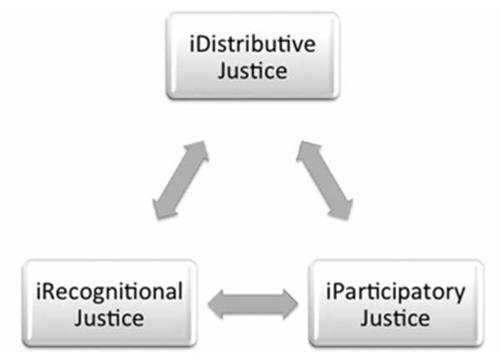
\includegraphics[width=3.5in,height=\textheight,keepaspectratio]{content/images/matiesen.png}

  }

  \caption{Source: (Mathiesen 2015)}

  \end{figure}%
\end{itemize}

Let us now consider these three components in a little more detail.

\subsection{Distribution}\label{distribution}

In her article, Mathiesen (2015) considers three distribution theories
and their relevance to the information perspective. The first is the
equal \textbf{distribution of personal satisfaction,} according to which
pleasure, satisfaction, and happiness are the goods that need to be
distributed equally between people. From this perspective, we should
strive to provide information to people in a way that satisfies their
needs and expectations. One issue is that people adjust their
expectations based on their experiences and environments, so applying
this model may reinforce inequalities by giving more to those who need
more by having more and less to those who need less by having less.
Another way to think of justice is to consider the equal
\textbf{distribution of resources}, with information being the resource
we would consider in the field. The problem with this approach is that
two people with the same amount of information may not benefit from it.
In a library where everyone has access to the same resources, some
patrons may not be able to use these resources to the same extent as
others. For example, a visually impaired person requires assistive
devices to access the resources. Finally, the equal \textbf{distribution
of capabilities} approach focuses on a person's capabilities instead of
their resources. These capabilities can be as simple as moving about,
meeting one's nutritional needs or acquiring clothing and shelter. So
here, we might think of how the distribution of information provides
everyone with the same level of capabilities.

\begin{tcolorbox}[enhanced jigsaw, arc=.35mm, bottomrule=.15mm, bottomtitle=1mm, breakable, colback=white, colbacktitle=quarto-callout-note-color!10!white, colframe=quarto-callout-note-color-frame, coltitle=black, left=2mm, leftrule=.75mm, opacityback=0, opacitybacktitle=0.6, rightrule=.15mm, title=\textcolor{quarto-callout-note-color}{\faInfo}\hspace{0.5em}{distributive Justice: A Real-World Example}, titlerule=0mm, toprule=.15mm, toptitle=1mm]

When Ontario locked down due to COVID-19 and sent all students home to
attend school virtually, there was a massive disconnect between students
with access to the internet and technologies. This was a clear case of a
digital divide preventing certain parts of society from access to
information. The Ontario government began an initiative to distribute
21,000 iPads and accessible data for school-aged children (ages 4-18).
In this case, internet access, and in turn access to information, is
considered a human right. Although this was a great initiative, there
were downfalls, the main one being that with over two million students
enrolled in Ontario schools, only 1\% were provided with iPads. This is
when 14\% of Ontario households were deemed to have slow or no internet
connectivity. One must question whether distributive justice was
achieved (Smith 2021).

\end{tcolorbox}

For Mathiesen (2015), the field needs to focus on \textbf{access}, which
she sees as a combination of resources (the information) and
capabilities (to use the information).

\begin{figure}[H]

{\centering 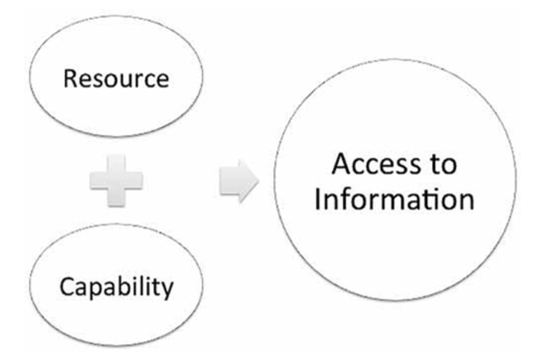
\includegraphics[width=3.82292in,height=\textheight,keepaspectratio]{content/images/mathiesen2.png}

}

\caption{Source: Mathiesen (2015)}

\end{figure}%

Thinking about access this way provides us with two main areas of
intervention to make information more accessible: acting on the
information itself or acting on the users or potential users. Here are
five factors that can help to determine whether information is
accessible to a particular group or person.

\textbf{Availability}: does the information exist?

\textbf{Findability}: can the information be found?

\textbf{Reachability}: can the seekers get the information?

\textbf{Comprehensibility}: can the information be understood?

\textbf{Usability}: is the information useful?

\begin{tcolorbox}[enhanced jigsaw, arc=.35mm, bottomrule=.15mm, bottomtitle=1mm, breakable, colback=white, colbacktitle=quarto-callout-tip-color!10!white, colframe=quarto-callout-tip-color-frame, coltitle=black, left=2mm, leftrule=.75mm, opacityback=0, opacitybacktitle=0.6, rightrule=.15mm, title=\textcolor{quarto-callout-tip-color}{\faLightbulb}\hspace{0.5em}{Pause and reflect}, titlerule=0mm, toprule=.15mm, toptitle=1mm]

\begin{itemize}
\tightlist
\item
  Can you consider other factors that information managers can consider
  to make information accessible?
\item
  How can we improve access to information by focusing on the users or
  potential users of information?
\item
  How can information be intellectually comprehensible but not
  physically comprehensible, and vice versa?
\item
  How can findability, availability and reachability issues affect
  unhoused and poor populations?
\end{itemize}

\end{tcolorbox}

\subsection{Participation}\label{participation}

The participation element of Mathiesen's informational justice framework
is related to the concept of participatory justice, which ``refers to
the direct participation of those affected most by a particular
decision, in the decision-making process itself: this could refer to
decisions made in a court of law or by policymakers''
(\href{https://en.wikipedia.org/wiki/Participatory_justice}{Wikipedia}).
In the realm of information, participatory justice thus refers to the
equal opportunity for people to participate in producing and
disseminating information.

\begin{tcolorbox}[enhanced jigsaw, arc=.35mm, bottomrule=.15mm, bottomtitle=1mm, breakable, colback=white, colbacktitle=quarto-callout-tip-color!10!white, colframe=quarto-callout-tip-color-frame, coltitle=black, left=2mm, leftrule=.75mm, opacityback=0, opacitybacktitle=0.6, rightrule=.15mm, title=\textcolor{quarto-callout-tip-color}{\faLightbulb}\hspace{0.5em}{Pause and reflect}, titlerule=0mm, toprule=.15mm, toptitle=1mm]

In the pre-digital world, the means of producing and disseminating
information were concentrated by media organizations and governments.
Now, the Internet and social media have levelled the playing field so
that anyone can have a voice and participate equally in producing and
disseminating information.

\begin{itemize}
\item
  What do you think of this statement? In what ways do you think it is
  accurate or not true?
\item
  Why do you think having equal access to producing and disseminating
  information matters?
\end{itemize}

\end{tcolorbox}

\subsection{Recognition}\label{recognition}

The recognition part of the informational justice framework emphasizes
the importance of respecting identities and cultural differences. To
help you think of recognitional justice from an information lens,
consider how negative stereotypes about certain groups or cultures can
be spread and reinforced in the news and social media through
informational processes. You may also find helpful to replace the term
recognition with representation and think of recognition justice as the
right for all people to be fairly represented in the informational
world. This idea celebrates the plurality of perspectives that are
constructed through discourse and that are to be considered equal, as
opposed to the idea of a single objective truth for us to know or the
existence of ``grand narratives'' that represent the dominant
perspective on the world and its history.

The
\href{https://www.rcaanc-cirnac.gc.ca/eng/1450124405592/1529106060525}{Truth
and Reconciliation Commission of Canada} is a good example of an attempt
to deconstruct a grand narrative about Canada's history and establish a
``new history'' of the country that better represents the lived
experiences and perspectives of Indigenous Peoples.

\begin{tcolorbox}[enhanced jigsaw, arc=.35mm, bottomrule=.15mm, bottomtitle=1mm, breakable, colback=white, colbacktitle=quarto-callout-tip-color!10!white, colframe=quarto-callout-tip-color-frame, coltitle=black, left=2mm, leftrule=.75mm, opacityback=0, opacitybacktitle=0.6, rightrule=.15mm, title=\textcolor{quarto-callout-tip-color}{\faLightbulb}\hspace{0.5em}{Pause and reflect}, titlerule=0mm, toprule=.15mm, toptitle=1mm]

Mathiesen (2015) emphasizes the interdependence of distributive,
participatory, and recognitional justice.

\begin{itemize}
\item
  How does distributive justice relate to participatory justice?
\item
  How does participatory justice relate to recognitional justice?
\item
  How does distributive justice relate to recognitional justice?
\item
  How do you think the three components of the framework come into play
  in the Truth and Reconciliation process?
\end{itemize}

\end{tcolorbox}

\section{Informational Justice in
Museums}\label{informational-justice-in-museums}

Museums are, traditionally, physical locations that serve a community by
collecting, preserving, and presenting cultural heritage objects.
However, museum institutions often come out of colonial contexts. When
considering informational justice in the museum sector, those colonial
pasts (and presents) must be examined and understood to pave the way for
a future where the information and objects that museums manage exemplify
justice, not bastions of inequality.

The collections of cultural heritage objects in many Canadian and
international museums are made up of objects removed from their cultures
and places of origin through dubious means or without consent. The
provenance of these items is sometimes hotly debated, and many
institutions are repatriating objects to their places/cultures of origin
to reflect modern mandates that support informational justice and
equality.

\begin{tcolorbox}[enhanced jigsaw, arc=.35mm, bottomrule=.15mm, bottomtitle=1mm, breakable, colback=white, colbacktitle=quarto-callout-note-color!10!white, colframe=quarto-callout-note-color-frame, coltitle=black, left=2mm, leftrule=.75mm, opacityback=0, opacitybacktitle=0.6, rightrule=.15mm, title=\textcolor{quarto-callout-note-color}{\faInfo}\hspace{0.5em}{In the news}, titlerule=0mm, toprule=.15mm, toptitle=1mm]

\url{https://www.browndailyherald.com/article/2022/11/risd-museum-returns-stolen-benin-bronze-sculpture-to-nigerian-national-collection}

\end{tcolorbox}

As information managers, we can also be critical of the information
surrounding cultural heritage objects inside museum spaces. For example,
many Canadian institutions displayed indigenous cultural heritage
objects alongside information that suggested the cultures of origin were
extinct when, in reality, many indigenous cultures are alive, resilient,
and thriving in the present day. Many exhibits are curated to display
certain cultures as foreign, and these exhibits are often curated
without the input of people relevant to those objects.

\begin{tcolorbox}[enhanced jigsaw, arc=.35mm, bottomrule=.15mm, bottomtitle=1mm, breakable, colback=white, colbacktitle=quarto-callout-tip-color!10!white, colframe=quarto-callout-tip-color-frame, coltitle=black, left=2mm, leftrule=.75mm, opacityback=0, opacitybacktitle=0.6, rightrule=.15mm, title=\textcolor{quarto-callout-tip-color}{\faLightbulb}\hspace{0.5em}{Pause and reflect}, titlerule=0mm, toprule=.15mm, toptitle=1mm]

How does this relate to Mathieson's Informational Justice Framework?

\end{tcolorbox}

Consider the following quotation from writer, poet, and community
organizer Jamara Wakefield:

\begin{quote}
Museums could be one of our greatest allies in liberation struggles.
They have the physical space, the means, and the public confidence to
partake in a large-scale social movement against colonial powers. Yet
they reject this opportunity over and over again. They prefer to remain
silent and hide in a world desperately needing decolonizing. (Wakefield
2019)
\end{quote}

Mike Murawski, author of Museums as Agents of Change, wrote the
following on how colonial culture affects many aspects of museums:

\begin{quote}
It dictates how people hold meetings together, who is invited to those
meetings, who participates, and whose ideas are valued. It dictates
decision-making in museum spaces. It controls how we define
``community,'' how we work with community partners and what we value
about those partners. White dominant culture dictates the words that get
written on museum websites and on the panels and labels in the
galleries, who gets to write, edit, and approve those words. (Murawski
2021)
\end{quote}

Murawski (2021) wrote the following points on Identifying and Replacing
White Dominant Culture In Museums:

\begin{itemize}
\item
  Move from professional and transactional relationships to
  relationships based on trust, care, and shared commitments.
\item
  Move from protecting power to sharing power.
\item
  Move from a culture of overworking to a culture of self-care and
  community care.
\item
  Move from competition and struggle for limited resources to a mindset
  of collaboration and working to share resources.
\item
  Move away from prioritizing only degrees, work experience, and job
  titles toward recognizing and centering lived experience.
\item
  Move from a place of those with power making decisions for others
  toward a place where we work to include those affected by decisions in
  the decision-making process.
\end{itemize}

\section{Case study}\label{case-study-8}

\emph{Tracy, in Halifax for a conference, meets with Jude for a coffee
to talk about Ava's experience with bullying and online harassment. They
discuss ways to address epistemic injustice and digital divides as Tracy
contemplates moving their family to the States.}

\textbf{Tracy}: Hey Jude, how have you been, old friend?

\textbf{Jude}: Hi Tracy! It's so lovely to see you! It's been a few
weeks since we've been able to catch up. I've just been buried deep in
the Archives, as usual. Honestly, that whole situation with the
podcaster made me step back from my side projects so I could think
deeply about everything. I might take a break from my blog for a bit.
How about you- how are you and Ava doing?

\textbf{Tracy}: I've been good. I am very busy with Ava, as usual. My
partner has been back in the Netherlands looking after his parents for
the last few months, so there's been a lot on my plate since I'm
essentially acting as a single parent.

\textbf{Jude}: That sounds like a lot. How has Ava's experience at
school been since she and her girlfriend went public?

\textbf{Tracy}: Over the past few weeks, the buzz around the school has
petered off, but they are still receiving hateful messages online. We've
been having many conversations lately about boundaries with social media
and ways they can manage their mental health. I tell Ava not to read the
messages she receives, but I know they significantly impact her whether
she reads them through or not. Delete and block, I say!

\textbf{Jude}: I am sorry to hear that. That is good advice- there is
nothing to be gained by reading those messages.

\textbf{Tracy}: I agree. However, Ava has voiced that she wants to
converse with them and present a different perspective. She is a lot
like you in some ways, Jude. She wants to do good and provide people
with information.

\textbf{Jude}: Well, she will be much better at it than I am. I think my
days of social justice blogging are behind me. I feel terrible that I
helped out that podcaster, and I think I need some time off. I'm sorry I
made it possible for them to speak their message. I guess it's more
painful now that I'm realizing how it affected my friends and their
families.

\textbf{Tracy}: Oh, but Jude, you didn't know what he was putting out
there- and your blog before was so well-received. It was educational,
and I know it inspired its readers to take positive action! Think of all
the great comments you used to get!

\textbf{Jude}: That is generous of you, Tracy. Over the past few weeks,
I've thought that many of my readers also came from places of privilege,
and I wasn't reaching the people I wanted to reach. My readership- they
have technology, they're educated. Ava inspires me; how do you reach
those who don't have access to the same perspectives or resources? How
do you introduce people to different ways of knowing and doing?

\textbf{Tracy}: That's a good point, Jude. Epistemic injustice runs deep
and is built into online structures just as it exists in the physical
institutions and places we inhabit. It can be even harder to spot online
because it is intangible, and the internet is so interconnected.
Information is changed and influenced on all sides. Users are creators,
authors, and audiences all at once. Ava's school has a class on digital
literacy where they discuss these themes. Their end-of-term project is
coming up, and we have been talking about them quite a bit- especially
in light of recent events!

\textbf{Jude}: Has Ava ever considered starting her podcast? It would be
an excellent idea for her and her classmates to discuss these things
openly and make them available for their peers and teachers to listen
to. It might help engage them all in conversation on these topics, and
as a new class begins each year, they could have multiple seasons!

\textbf{Tracy}: What a fascinating idea, Jude! See- we can't keep you
from trying to help others! While I think that has real potential, I am
not sure Ava's school has the technological infrastructure to support an
initiative like that. The digital divide is quite poignant in our town-
the schoolboard doesn't have the resources to keep up with advancing
technical change. Their school only got open Wi-Fi last year!

\textbf{Jude}: Hmm\ldots{} well\ldots{} now that my podcasting days are
behind me, I'd like to redirect that effort somewhere that is needed. I
have a ton of equipment in my studio, and I'd be happy to gift it to
Ava's school to get a project like this off the ground. I could even
teach a few workshops on using the equipment and set them up with
essential software to record episodes.

\textbf{Tracy}: I'm sure they would be happy to hear from you- why don't
I see if I can put you in touch? It's great to have the old Jude back;
this sounds more like him! Ok, Jude - stay out of trouble. Thanks for
meeting me here at the hotel for a coffee. I'd better check on Ava and
then wrap up the conference. We're taking a red eye out of here tonight.
I'll see you in Canmore?

\textbf{Jude}: Good to see you, Tracy. Thanks for chatting. Yes, I'll be
in Canmore - I'm excited to get everyone together again!

\emph{Many changes are on the horizon for each character, and with the
fifth anniversary of their time at Dalhousie, they've decided to come
together in Canmore, Alberta, for a celebratory trip. The four of them
are out for a nice dinner on a patio overlooking the mountains,
discussing their plans.}

\textbf{Dante}: Thank you so much for planning this trip, Tracy! I'm so
happy to have a relaxing vacation before my big move. I'm glad we chose
a convenient location; the drive from Saskatoon wasn't too bad.

\textbf{Tracy}: I'm so happy it worked out! It's been a while since all
four of us have been together, and this seemed like the perfect
opportunity. I'm glad we were all able to get vacation time set aside.

\textbf{Jude}: This was the perfect idea. The mountains are so gorgeous,
and some outdoor therapy can never hurt.

\textbf{Wren}: So true! Tell us about your new job, Dante! We're all so
proud of you; this is such a big move for you.

\textbf{Dante}: Well, as you know, I'll be working as the Chief
Librarian at Iqaluit Centennial Library in Nunavut. My dream's always
been to run a library, so I'm super excited about this new chapter.
There's so much I want to do there, but the number one thing I want to
accomplish is closing the digital divide. There are so many access
issues in Northern Canada. I want to create programming to teach
children about digital literacy and help them through issues they may be
dealing with, like online bullying.

\textbf{Wren}: Dante, that is so lovely! That sounds like the perfect
job for you. Tracy, how are things with your job?

\textbf{Tracy}: There have been some significant changes in my company.
They've hired a Black female CEO recently, and so many positive changes
have already occurred. I'm looking forward to seeing what new ways the
company will work to promote equity. And you, Wren? You're still at the
same job.

\textbf{Wren}: I am! I've been there for about five years now, which
seems crazy! Things are pretty steady at work, but a few months ago, I
started a non-profit organization that helps to provide internships and
mentorship for women in tech. I'm so excited to be able to help a new
generation of women find their passion in this field. What about you,
Jude? Is anything exciting happening at the archives?

\textbf{Jude}: That's inspiring, Wren; you will make a difference for
many young women. We just received a large grant from the government to
work towards truth and reconciliation. I'm excited to work with the
local Indigenous communities to find a way to improve the archives. On a
similar note, I'm also consulting for Dante in establishing digital
literacy programming. The podcasting initiative at Ava's school was so
successful and in demand from the students that the school was given a
large grant by the province to set up more technical infrastructure.
Donations from readers on my blog didn't hurt either. We will draw from
our experiences setting up that programming to address access issues in
Iqaluit.

\textbf{Dante}: Looks like things are going well all around. It's been a
crazy few years, but I'm glad we all met! Cheers to many more years!

{[}Glasses clink together in a sunlit shot with the mountains in the
background in a Polaroid-perfect moment.{]}

\section{Discussion Questions}\label{discussion-questions-7}

\begin{itemize}
\item
  How do you interpret Knowledge versus Information justice? What are a
  few examples of this you can think of?
\item
  Have you experienced digital divides in your own life? What digital
  divides can you identify in your community? In your province? In
  Canada? Across the globe? Can you identify any possible solutions for
  closing these divides?
\item
  How do digital divides create unequal footing regarding information
  literacy and access to information?
\item
  What sort of digital divides exist in rural areas and urban centres?
  What sort of divides exist between them?
\item
  Consider how digital divides in Canada occur systemically, especially
  regarding Indigenous communities.
\item
  Relate the case study to Mathiesen's Informational Justice Framework,
  including distributive justice, participatory justice, and
  recognitional justice.
\item
  Reflect on what you have learned throughout the last semester and
  think through the course themes.
\end{itemize}

\section*{References}\label{references-10}
\addcontentsline{toc}{section}{References}

\protect\phantomsection\label{refs}
\begin{CSLReferences}{1}{1}
\bibitem[\citeproctext]{ref-albrecht2006}
Albrecht, Steffen. 2006. {``Whose Voice Is Heard in Online
Deliberation?: A Study of Participation and Representation in Political
Debates on the Internet.''} \emph{Information, Communication \& Society}
9 (1): 62--82. \url{https://doi.org/10.1080/13691180500519548}.

\bibitem[\citeproctext]{ref-al-sharieh_securing_2018}
Al-Sharieh, Saleh. 2018. {``Securing the {Future} of {Copyright}
{Users}' {Rights} in {Canada}.''} \emph{Windsor Yearbook of Access to
Justice} 35 (May): 11--39.
\url{https://doi.org/10.22329/wyaj.v35i0.5109}.

\bibitem[\citeproctext]{ref-appleton2022}
Appleton, Leo, and Hazel Hall. 2022. {``The Public Library as Public
Sphere: A Longitudinal Analysis.''} \emph{Journal of Documentation},
ahead of print, May 9. \url{https://doi.org/10.1108/JD-02-2022-0031}.

\bibitem[\citeproctext]{ref-audunson2019}
Audunson, Ragnar, Svanhild Aabø, Roger Blomgren, et al. 2019. {``Public
Libraries as an Infrastructure for a Sustainable Public Sphere: A
Comprehensive Review of Research.''} \emph{Journal of Documentation} 75
(4): 773--90. \url{https://doi.org/10.1108/JD-10-2018-0157}.

\bibitem[\citeproctext]{ref-bates2006}
Bates, Marcia J. 2006. {``Fundamental Forms of Information.''}
\emph{Journal of the American Society for Information Science and
Technology} 57 (8): 10331045. \url{https://doi.org/10.1002/asi.20369}.

\bibitem[\citeproctext]{ref-bates2015}
Bates, Marcia J. 2015. {``The Information Professions: Knowledge,
Memory, Heritage.''} \emph{Information Research} 20 (1): Paper 665.
\url{http://informationr.net/ir/20-1/paper655.html}.

\bibitem[\citeproctext]{ref-bawden_dark_2009}
Bawden, David, and Lyn Robinson. 2009. {``The Dark Side of Information:
Overload, Anxiety and Other Paradoxes and Pathologies.''} \emph{Journal
of Information Science} 35 (2): 180--91.
\url{https://doi.org/10.1177/0165551508095781}.

\bibitem[\citeproctext]{ref-benselin_information_2016}
Benselin, Jennifer C, and Gillian Ragsdell. 2016. {``Information
Overload: {The} Differences That Age Makes.''} \emph{Journal of
Librarianship and Information Science} 48 (3): 284--97.
\url{https://doi.org/10.1177/0961000614566341}.

\bibitem[\citeproctext]{ref-bhandari2022}
Bhandari, Aparajita, and Sara Bimo. 2022. {``Why{'}s Everyone on TikTok
Now? The Algorithmized Self and the Future of Self-Making on Social
Media.''} \emph{Social Media + Society} 8 (1): 205630512210862.
\url{https://doi.org/10.1177/20563051221086241}.

\bibitem[\citeproctext]{ref-bran_learning_2021}
Bran, Ramona, Laurentiu Tiru, Gabriela Grosseck, Carmen Holotescu, and
Laura Malita. 2021. {``Learning from {Each} {Other}---{A} {Bibliometric}
{Review} of {Research} on {Information} {Disorders}.''}
\emph{Sustainability} 13 (18): 10094.
\url{https://doi.org/10.3390/su131810094}.

\bibitem[\citeproctext]{ref-brin2021}
Brin, Lise. 2021. \emph{Expenditures of CARL Member Libraries for
Scholarly Resource Subscriptions Licensed Through CRKN for 2019 - 2020 /
Dépenses Des Bibliothèques Membres de l'ABRC Pour Les Abonnements Aux
Ressources Savantes Sous Licence Du RCDR Pour l'année 2019 - 2020}.
Federated Research Data Repository / dépôt fédéré de données de
recherche. \url{https://doi.org/10.20383/102.0324}.

\bibitem[\citeproctext]{ref-buckland1991}
Buckland, MK. 1991. {``Information as Thing.''} \emph{JASIS}.
\url{http://skat.ihmc.us/rid=1KR7VC4CQ-SLX5RG-5T39/BUCKLAND(1991)-informationasthing.pdf}.

\bibitem[\citeproctext]{ref-butler2022}
Butler, Leigh-Ann, Lisa Matthias, Marc-André Simard, Philippe Mongeon,
and Stefanie Haustein. 2022. \emph{The Oligopoly's Shift to Open Access.
How For-Profit Publishers Benefit from Article Processing Charges}.
\url{https://doi.org/10.5281/zenodo.7057144}.

\bibitem[\citeproctext]{ref-bystruxf6m2019}
Byström, Katriina, Jannica Heinström, and Ian Ruthven. 2019.
\emph{Information at work: information management in the workplace}.
Facet Publishing.

\bibitem[\citeproctext]{ref-choo2005}
Choo, Chun Wei. 2005. \emph{The Knowing Organization}. Oxford University
Press. \url{https://doi.org/10.1093/acprof:oso/9780195176780.001.0001}.

\bibitem[\citeproctext]{ref-choo_knowing_2006}
Choo, Chun Wei. 2006. {``The Knowing Organization.''} In \emph{The
Knowing Organization: How Organizations Use Information to Construct
Meaning, Create Knowledge, and Make Decisions}, 2nd ed. Oxford
University Press.

\bibitem[\citeproctext]{ref-depaor2020}
De Paor, Saoirse, and Bahareh Heravi. 2020. {``Information Literacy and
Fake News: How the Field of Librarianship Can Help Combat the Epidemic
of Fake News.''} \emph{The Journal of Academic Librarianship} 46 (5):
102218. \url{https://doi.org/10.1016/j.acalib.2020.102218}.

\bibitem[\citeproctext]{ref-draper_corporate_2019}
Draper, Nora A, and Joseph Turow. 2019. {``The Corporate Cultivation of
Digital Resignation.''} \emph{New Media \& Society} 21 (8): 1824--39.
\url{https://doi.org/10.1177/1461444819833331}.

\bibitem[\citeproctext]{ref-fischer2008}
Fischer, Frank. 2008. {``Local Science Vs Global Science: Approaches to
Indigenous Knowledge in International Development.''}
\emph{ENVIRONMENTAL POLITICS} 17 (5): 853--55.

\bibitem[\citeproctext]{ref-gorman2015}
Gorman, Michael. 2015. \emph{Our Enduring Values Revisited:
Librarianship in an Ever-Changing World}. ALA Editions, an imprint of
the American Library Association.

\bibitem[\citeproctext]{ref-habermas1999}
Habermas, Jürgen. 1999. \emph{The Structural Transformation of the
Public Sphere: An Inquiry into a Category of Bourgeois Society}. 10.
print. Studies in Contemporary German Social Thought. MIT Press.

\bibitem[\citeproctext]{ref-hjorland_information_2007}
Hjørland, Birger. 2007. {``Information: {Objective} or
Subjective/Situational?''} \emph{Journal of the American Society for
Information Science and Technology} 58 (10): 1448--56.
\url{https://doi.org/10.1002/asi.20620}.

\bibitem[\citeproctext]{ref-kelly2008}
Kelly, Kevin. 2008. \emph{Better Than Free}.
\url{https://www.edge.org/conversation/better-than-free}.

\bibitem[\citeproctext]{ref-koehler2003}
Koehler, Wallace. 2003. {``Professional Values and Ethics as Defined by
{"}the LIS Discipline{"}.''} \emph{Journal of Education for Library and
Information Science} 44 (2): 99--119.
\url{http://cat.inist.fr/?aModele=afficheN&cpsidt=15045134}.

\bibitem[\citeproctext]{ref-kokolakis2017}
Kokolakis, Spyros. 2017. {``Privacy Attitudes and Privacy Behaviour: A
Review of Current Research on the Privacy Paradox Phenomenon.''}
\emph{Computers \& Security} 64 (January): 122--34.
\url{https://doi.org/10.1016/j.cose.2015.07.002}.

\bibitem[\citeproctext]{ref-lariviuxe8re2015}
Larivière, Vincent, Stefanie Haustein, and Philippe Mongeon. 2015.
{``The Oligopoly of Academic Publishers in the Digital Era.''}
\emph{PLOS ONE} 10 (6): e0127502.
\url{https://doi.org/10.1371/journal.pone.0127502}.

\bibitem[\citeproctext]{ref-lee_towards_2021}
Lee, Ashlin. 2021. {``Towards {Informatic} {Personhood}: Understanding
Contemporary Subjects in a Data-Driven Society.''} \emph{Information,
Communication \& Society} 24 (2): 167--82.
\url{https://doi.org/10.1080/1369118X.2019.1637446}.

\bibitem[\citeproctext]{ref-lewandowsky_misinformation_2012}
Lewandowsky, Stephan, Ullrich K. H. Ecker, Colleen M. Seifert, Norbert
Schwarz, and John Cook. 2012. {``Misinformation and {Its} {Correction}:
{Continued} {Influence} and {Successful} {Debiasing}.''}
\emph{Psychological Science in the Public Interest} 13 (3): 106--31.
\url{https://doi.org/10.1177/1529100612451018}.

\bibitem[\citeproctext]{ref-mathiesen2015}
Mathiesen, Kay. 2015. {``Informational Justice: A Conceptual Framework
for Social Justice in Library and Information Services.''} \emph{Library
Trends} 64 (2): 198225. \url{https://doi.org/10.1353/lib.2015.0044}.

\bibitem[\citeproctext]{ref-matthes_too_2020}
Matthes, Jörg, Kathrin Karsay, Desirée Schmuck, and Anja Stevic. 2020.
{``{`{Too} Much to Handle'}: {Impact} of Mobile Social Networking Sites
on Information Overload, Depressive Symptoms, and Well-Being.''}
\emph{Computers in Human Behavior} 105 (April): 106217.
\url{https://doi.org/10.1016/j.chb.2019.106217}.

\bibitem[\citeproctext]{ref-mckee2004}
McKee, Alan. 2004. \emph{The Public Sphere: An Introduction}. Cambridge
University Press. \url{https://doi.org/10.1017/CBO9780511819339}.

\bibitem[\citeproctext]{ref-misra_psychological_2012}
Misra, Shalini, and Daniel Stokols. 2012. {``Psychological and {Health}
{Outcomes} of {Perceived} {Information} {Overload}.''} \emph{Environment
and Behavior} 44 (6): 737--59.
\url{https://doi.org/10.1177/0013916511404408}.

\bibitem[\citeproctext]{ref-mongeon2023}
Mongeon, Philippe, Catherine Gracey, Poppy Riddle, Madelaine Hare,
Marc-André Simard, and Jean-Sébastien Sauvé. 2023. {``Mapping
Information Research in Canada.''} \emph{The Canadian Journal of
Information and Library Science} 46 (2): 1--27.
\url{https://doi.org/10.5206/cjils-rcsib.v46i2.15568}.

\bibitem[\citeproctext]{ref-mongeon2021}
Mongeon, Philippe, Kyle Siler, Antoine Archambault, Cassidy Sugimoto,
and Vincent Larivière. 2021. {``Collection Development in the Era of Big
Deals.''} \emph{College \& Research Libraries} 82 (2): 219.
\url{https://doi.org/10.5860/crl.82.2.219}.

\bibitem[\citeproctext]{ref-morrison2021}
Morrison, Sara. 2021. \emph{Think You Have Nothing to Hide? Why You
Should Care about Data Privacy Anyway.}
\url{https://www.vox.com/recode/22250897/facebook-data-privacy-collection-algorithms-extremism}.

\bibitem[\citeproctext]{ref-muir2010}
Muir, Gordon, and Holly Heller-Ross. 2010. {``Is Embedded Librarianship
Right for Your Institution?''} \emph{Public Services Quarterly} 6 (2-3):
92--109. \url{https://doi.org/10.1080/15228959.2010.497464}.

\bibitem[\citeproctext]{ref-murawski2021}
Murawski, Michael. 2021. \emph{Museums as Agents of Change: A Guide to
Becoming a Changemaker}. Rowman \& Littlefield.

\bibitem[\citeproctext]{ref-naveed_towards_2020}
Naveed, Muhammad Asif. 2020. {``Towards {Information} {Anxiety} and
{Beyond}.''} \emph{Webology} 17 (1): 65--80.
\url{https://doi.org/10.14704/WEB/V17I1/a208}.

\bibitem[\citeproctext]{ref-panch2019}
Panch, Trishan, Heather Mattie, and Rifat Atun. 2019. {``Artificial
Intelligence and Algorithmic Bias: Implications for Health Systems.''}
\emph{Journal of Global Health} 9 (2): 010318.
\url{https://doi.org/10.7189/jogh.09.020318}.

\bibitem[\citeproctext]{ref-papacharissi_without_2012}
Papacharissi, Zizi. 2012. {``Without {You}, {I}'m {Nothing}:
{Performances} of the {Self} on {Twitter}.''} \emph{International
Journal of Communication} 6 (0): 18.
\url{https://ijoc.org/index.php/ijoc/article/view/1484}.

\bibitem[\citeproctext]{ref-pasquale2018}
Pasquale, Frank. 2018. \emph{The Automated Public Sphere}. Routledge.

\bibitem[\citeproctext]{ref-radicatigroup2021}
Radicati Group. 2021. \emph{Email Statistics Report, 2021-2025}. London.

\bibitem[\citeproctext]{ref-rowley2007}
Rowley, Jennifer. 2007. {``The Wisdom Hierarchy: Representations of the
DIKW Hierarchy.''} \emph{Journal of Information Science}, ahead of
print, February 15. \url{https://doi.org/10.1177/0165551506070706}.

\bibitem[\citeproctext]{ref-senge2006}
Senge, Peter M. 2006. \emph{The Fifth Discipline: The Art and Practice
of the Learning Organization}. Rev. and updated. Doubleday/Currency.

\bibitem[\citeproctext]{ref-shu2017}
Shu, Fei, Philippe Mongeon, Stefanie Haustein, Kyle Siler, Juan Pablo
Alperin, and Vincent Larivière. 2017. {``Is It Such a Big Deal? On the
Cost of Journal Use in the Digital Era.''} \emph{College and Research
Libraries}.

\bibitem[\citeproctext]{ref-shumaker_defining_2012}
Shumaker, David. 2012a. {``Defining Embedded Librarianship.''} In
\emph{The {Embedded} {Librarian}: Innovative Strategies for Taking
Knowledge Where It's Needed}. Information Today, Inc.

\bibitem[\citeproctext]{ref-shumaker2012}
Shumaker, David. 2012b. \emph{Push and Pull : The Forces Driving
Embedded Librarianship}. Information Today, Inc.

\bibitem[\citeproctext]{ref-simon1971}
Simon, Herbert A. 1971. {``Designing Organizations for an
Information-Rich World.''} \emph{Computers, Communications, and the
Public Interest} 72: 37.

\bibitem[\citeproctext]{ref-smith_ipads_2021}
Smith, Karen Louise. 2021. {``{iPads}, {Free} {Data} and {Young}
{Peoples}' {Rights}: {Refractions} from a {Universal} {Access} {Model}
{During} the {Pandemic}.''} \emph{Studies in Social Justice} 15 (3):
414--41. \url{https://doi.org/10.26522/ssj.v15i3.2509}.

\bibitem[\citeproctext]{ref-somphanpae2016}
Somphanpae, Salinthip, and Somjai Boonsiri. 2016. {``Business Process
Improvement Using Adjustable Parameters on Simulation{\textendash}a Case
Study in Restaurant Business.''} \emph{Journal of Advances in
Information Technology}, 232--38.
\url{https://doi.org/10.12720/jait.7.4.232-238}.

\bibitem[\citeproctext]{ref-sparks_what_2013}
Sparks, Colin. 2013. {``What Is the {`{Digital} {Divide}'} and Why Is It
{Important}?''} \emph{Javnost - The Public} 20 (2): 27--46.
\url{https://doi.org/10.1080/13183222.2013.11009113}.

\bibitem[\citeproctext]{ref-star_power_1990}
Star, Susan Leigh. 1990. {``Power, {Technology} and the {Phenomenology}
of {Conventions}: {On} Being {Allergic} to {Onions}.''} \emph{The
Sociological Review} 38 (1\_suppl): 26--56.
\url{https://doi.org/10.1111/j.1467-954X.1990.tb03347.x}.

\bibitem[\citeproctext]{ref-wakefield2019}
Wakefield, Jamara. 2019. \emph{Museums Could Be Powerful, Liberatory
Spaces If They Let Go of Their Colonial Practices}.
\url{https://racebaitr.com/2019/05/14/museums-could-be-powerful-liberatory-spaces-if-they-let-go-of-their-colonial-practices/}.

\bibitem[\citeproctext]{ref-webster_definitions_2014}
Webster, Frank. 2014a. {``Definitions.''} In \emph{Theories of the
Information Society}, Fourth edition. International Library of
Sociology. Routledge.

\bibitem[\citeproctext]{ref-webster_information_2014-1}
Webster, Frank. 2014b. {``Information and Democracy 1: {Jürgen}
{Habermas}, the Public Sphere and Public Service Institutions.''} In
\emph{Theories of the Information Society}, Fourth edition.
International Library of Sociology. Routledge.

\bibitem[\citeproctext]{ref-webster_information_2014}
Webster, Frank. 2014c. {``Information and the Market System: {Herbert}
{Schiller}.''} In \emph{Theories of the Information Society}, Fourth
edition. International Library of Sociology. Routledge.

\bibitem[\citeproctext]{ref-webster_information_2014-2}
Webster, Frank. 2014d. {``Information, Reflexivity and Surveillance:
{Anthony} {Giddens}.''} In \emph{Theories of the Information Society},
Fourth edition. International Library of Sociology. Routledge.

\bibitem[\citeproctext]{ref-webster_network_2014}
Webster, Frank. 2014e. {``Network Society: {Manuel} {Castells}.''} In
\emph{Theories of the Information Society}, Fourth edition.
International Library of Sociology. Routledge.

\bibitem[\citeproctext]{ref-weichoo2001}
Wei Choo, Chun. 2001. {``The Knowing Organization as Learning
Organization.''} \emph{Education + Training} 43 (4/5): 197--205.
\url{https://doi.org/10.1108/eum0000000005482}.

\bibitem[\citeproctext]{ref-widdersheim2016}
Widdersheim, Michael M. 2016. {``Late, Lost, or Renewed? A Search for
the Public Sphere in Public Libraries.''} \emph{Information Research} 22
(1).

\bibitem[\citeproctext]{ref-york2019}
York, Jillian, and Ethan Zuckerman. 2019. \emph{Moderating the Public
Sphere}. The MIT Press.
\url{https://doi.org/10.7551/mitpress/11304.003.0012}.

\end{CSLReferences}




\end{document}
